\documentclass[11pt]{article}
\usepackage[T1]{fontenc}
\usepackage{lmodern}
\usepackage[letterpaper,width=6.12in,height=8.98in,
  top=1.05in,headheight=14pt,headsep=20pt]{geometry}
\usepackage{amsthm,mathtools,amssymb}
\usepackage{microtype}
\usepackage{booktabs,enumitem}
\usepackage{tikz}
\usetikzlibrary{arrows.meta,calc,positioning}
\usepackage[font=small,labelfont=bf,labelsep=period]{caption}
\usepackage{fancyhdr}
\usepackage{bookmark} % loads hyperref
\input glyphtounicode
\pdfgentounicode=1

\definecolor{ink}{HTML}{213650}
\definecolor{lagoon}{HTML}{175967}
\definecolor{ember}{HTML}{994121}
\hypersetup{pdftitle={Strongly polynomial linear programming},pdfauthor={OpenAI},
 pdfsubject={Strongly-polynomial-linear-programming-November-24-2026},
 colorlinks=true,linkcolor=ink,citecolor=lagoon,urlcolor=lagoon,bookmarksopen=true,bookmarksopenlevel=1}

\linespread{1.025}
\raggedbottom
\setlist[itemize,enumerate]{topsep=4pt plus 1pt,itemsep=2pt,parsep=0pt}
\setlength{\textfloatsep}{14pt plus 3pt minus 3pt}
\emergencystretch=0.8em
\setcounter{tocdepth}{1}
\makeatletter
\renewcommand{\maketitle}{%
  \begin{center}
    {\@title\par}\vspace{6pt}
    {\normalfont\large\@author\par}\vspace{2pt}
    {\normalfont\normalsize\@date\par}
  \end{center}\thispagestyle{plain}}

\newcommand{\contents}{%
 \begin{center}{\small\bfseries\contentsname}\end{center}
 \vspace{-6pt}
 \begingroup
 \renewcommand*\l@section[2]{%
   \setlength\@tempdima{2em}%
   \par\addvspace{6pt}\noindent
   \makebox[\textwidth]{\hskip2.5em ##1\hfill ##2\hskip2.5em\relax}\par}
 \@starttoc{toc}
 \endgroup}
\makeatother
\pagestyle{fancy}
\fancyhf{}
\fancyhead[L]{\small\color{black!63}\nouppercase{\leftmark}}
\fancyhead[R]{\small\thepage}
\renewcommand{\headrulewidth}{0pt}
\renewcommand{\sectionmark}[1]{\markboth{\thesection.\ #1}{}}
\widowpenalty=6000
\clubpenalty=3000
\displaywidowpenalty=4000

\numberwithin{equation}{section}
\newtheorem{theorem}{Theorem} % global
\newtheorem{proposition}[theorem]{Proposition}
\newtheorem{corollary}[theorem]{Corollary}
\newtheorem{lemma}{Lemma}[section]
\newtheorem{claim}[lemma]{Claim}
\theoremstyle{definition}
\newtheorem{remark}[lemma]{Remark}
\newtheorem{definition}[lemma]{Definition}

\newcommand{\ddref}[1]{\textup{(\ref{#1})}}
\DeclareMathOperator{\supp}{supp}
\DeclareMathOperator{\rank}{rank}
\DeclareMathOperator{\sgn}{sgn}
\DeclareMathOperator{\tr}{tr}
\DeclareMathOperator{\poly}{poly}
\newcommand{\RR}{\mathbb R}
\newcommand{\QQ}{\mathbb Q}
\newcommand{\ZZ}{\mathbb Z}
\newcommand{\NN}{\mathbb N}
\newcommand{\EE}{\mathbb E}
\newcommand{\PP}{\mathbb P}
\newcommand{\Slots}{\mathcal S}

\title{\fontsize{21}{25}\selectfont\bfseries\color{ink}Strongly polynomial linear programming}
\author{OpenAI}
\date{November 24, 2026}

\begin{document}
\maketitle

\begin{abstract}
\normalsize\noindent
We give a deterministic strongly polynomial algorithm for linear programming,
answering Smale's ninth problem. For arbitrary real coefficients, the number of
steps is bounded by a polynomial in the numbers of variables and constraints.
For rational data, every intermediate number has bit length polynomial in the binary input length.
The method also gives a strongly polynomial algorithm for convex quadratic
programming. For finite turn-based mean-payoff games with perfect information,
it gives strongly polynomial time for deterministic games and polynomial bit
time for stochastic games with binary rational data.

\end{abstract}

\section{Introduction}\label{sec:introduction}

How much work does it take to optimize a linear function subject to linear
inequalities? For rational coefficients, the ellipsoid method of
Khachiyan~\cite{Khach,Khach2} gave an answer polynomial in the length of the
input. Two linear programs with the same numbers of variables and constraints
can have very different input lengths. Megiddo~\cite{MegEnc,Meg} asked
whether those two dimensions alone could bound the number of arithmetic
operations. Tarjan raised the question for real data~\cite[pp.~1620--1621]{Tari},
and Smale made it his ninth problem~\cite{Smale}. We give an affirmative answer.

We maximize \(c^\top x\) subject to \(Ax\le b\), given
\(A\in\RR^{m\times n}\), \(b\in\RR^m\) and \(c\in\RR^n\) explicitly.
A \emph{strongly polynomial} algorithm takes polynomially many steps
in \(m,n\), counting exact scalar arithmetic, comparisons and control work.
On rational input every intermediate number has bit length polynomial in
the full binary input length.

\begin{theorem}[Strongly polynomial linear programming]\label{thm:lp}
For arbitrary real \(A,b,c\), a deterministic strongly polynomial algorithm
returns one of the following certificates for \(\max\{c^\top x:Ax\le b\}\).
\begin{enumerate}
 \item \emph{Finite optimum.} A strictly complementary primal--dual pair \(x,y\) with
 \[
    s=b-Ax\ge0,\qquad y\ge0,\qquad A^\top y=c,\qquad
    s^\top y=0,\qquad s+y>0 .
 \]
 \item \emph{Unbounded objective.} A feasible point \(x\) and an improving ray
 \(r\) with \(Ar\le0\) and \(c^\top r>0\).
 \item \emph{Infeasibility.} A vector \(y\ge0\) with \(A^\top y=0\),
 \(b^\top y<0\), and \(\lvert\supp y\rvert\le 1+\rank A\).
\end{enumerate}
\end{theorem}

We use a uniform sequential model~\cite{BSS}. The scalar operations are
addition, subtraction, multiplication, division by a nonzero scalar,
comparison and copying, with constants \(0,1\). Control operations on
indices and explicit bit strings are charged at bit cost. The algorithm accesses scalar inputs only through the scalar operations.
All vector inequalities are componentwise. On rational data we measure a
number by its reduced fraction.

The arithmetic result extends to every ordered field. In particular, on
rational input the certificates are exact rationals. If the input is supplied
as integer numerator--denominator pairs, an implementation also keeps the
integers in its unreduced pairs of polynomial bit length throughout the
computation (Section~\ref{sec:arithmetic}).

\paragraph{How the algorithm finds a certificate.}
Consider first the feasibility of \(Ax\le b\). A feasible point has
nonnegative slacks \(b-Ax\). A certificate of infeasibility instead gives
nonnegative weights for a combination of the inequalities that yields a
contradiction. Homogenizing the slack vectors puts these alternatives in
two orthogonal subspaces. To decide feasibility it suffices to determine
which subspace contains a nonnegative vector positive at one designated
coordinate.

A positive entry of such a vector can be arbitrarily small compared with its
largest entry. Changing the unit of a coordinate changes which entries can be
seen at a fixed precision. The algorithm uses these changes of unit as
queries. At each query it obtains reliable signs where the rescaled entries
are largest. A search combining the signs from different queries identifies
the subspace containing a witness, even though the algorithm does not know
in advance which signs it can trust. It then sets coordinates to zero, one
at a time whenever a witness survives, until linear algebra recovers the
witness exactly.

The difficulty is making each query affordable. For a witness of minimal support,
the ratios of its nonzero entries are ratios of subdeterminant magnitudes
of a basis matrix for the two subspaces. Even in a fixed dimension, the
logarithms of these magnitudes can be arbitrarily far apart.
The algorithm gives short substitutes for the logarithms as they are
needed, preserving the comparisons that determine which entries are large.
This lets it compute each set of signs using ordinary polynomial-time LP
on rational data whose bit lengths are bounded in the dimensions alone.
Section~\ref{sec:overview} explains how the search, the changes of unit and
the compression fit together.

\subsection{Consequences}

The same search applies to a convex quadratic objective under linear
constraints. For arbitrary real coefficients we find an exact minimizer
and its multipliers, or certify infeasibility or unboundedness, in
deterministic strongly polynomial time (Corollary~\ref{cor:qp}).
The underlying result solves the monotone linear complementarity problem.
Given \(M,q\) with \(M+M^\top\) positive semidefinite, it finds \(z\ge0\)
such that \(Mz+q\ge0\) and \(z^\top(Mz+q)=0\), or certifies that no
such \(z\) exists (Theorem~\ref{thm:lcp}).

There is a second use for the signs returned by a query. If a point differs
from the fixed point of a contraction in max norm, the map moves it toward
that fixed point in every coordinate of greatest error. For a self-map of
\([-1,1]^n\) with Lipschitz constant at most \(1-2^{-b}\), this gives a
deterministic algorithm that locates the fixed point to within \(2^{-k}\)
in time polynomial in \(n,b,k\), counting all bits exchanged with the
evaluation oracle (Theorem~\ref{thm:contraction}).

In a finite turn-based mean-payoff game, two players with perfect information
choose moves on a graph. One maximizes and the other minimizes the long-run
average reward. The fixed-point algorithm and policy evaluation by LP give the exact values
from every starting vertex and optimal strategies for both players. The running time
is strongly polynomial when each move has a deterministic outcome and
polynomial in the binary input length when outcomes are stochastic and the
data rational. This includes polynomial time for simple stochastic reachability
games. Theorem~\ref{thm:games} gives the bounds for arbitrary real rewards
and for discounted play.

\subsection{Earlier approaches to strongly polynomial time}
\label{sec:lp-context}

The first polynomial-time algorithms for general linear programming
measure the size of a rational instance in bits. Khachiyan's ellipsoid
algorithm~\cite{Khach,Khach2} draws on the cutting-plane methods of
Shor and Yudin--Nemirovskii~\cite{Shor,YN}. In its feasibility argument,
the volume of the enclosing ellipsoid falls by a controlled factor at
each cut. Determinant bounds in terms of the input length tell the
algorithm when that volume is too small to contain a feasible region
of the required thickness~\cite{GLS}. Karmarkar's projective
algorithm~\cite{Kar} gave a second route to polynomial bit complexity.
Subsequent interior-point methods follow solutions of penalized problems
as the penalty for approaching the boundary decreases~\cite{NN}.
Faster linear algebra reduces the work per solve~\cite{Ren,Vai,CLS,VDB},
while exact recovery still has to account for the input
precision~\cite{GPV}. Even on the interval $[0,1]$, the objective
$x\mapsto 2^{-L}x$ gives the two vertices values only $2^{-L}$ apart.
Intervals of radius $2^{-k}$ around these values are disjoint only for
$k>L+1$. A single exact sign comparison selects the optimal endpoint.

\paragraph{Removing dependence on the data.}
Tardos first obtained a strongly polynomial algorithm for minimum-cost
circulation~\cite{TarCirc}, then showed that the arithmetic operation
count for a rational LP can depend on the encoding length of the
constraint matrix alone~\cite{Tardos}. This gives a strongly polynomial
bound whenever the entries of the matrix have polynomial encoding length
in the dimensions, including matrices with entries in $\{0,1,-1\}$.
Frank and Tardos~\cite{FT} replace a vector by a short integer vector
whose inner products with bounded integer vectors have the same signs.
When the constraint matrix has short entries, this lets one compress
the objective and the right-hand side while preserving the comparisons
needed for optimization~\cite[\S6.6]{GLS}.

A different source of strongly polynomial bounds is structure in the
constraint matrix. Megiddo solved LP in linear time for fixed
dimension~\cite{MegLin}, and solved feasibility for inequalities
involving at most two variables each~\cite{Meg}. Generalized flow
maximization supplies a related class with at most two nonzeros per
column~\cite{Vegh,OV}. Dadush, Koh, Natura, Olver and V\'egh obtained a
strongly polynomial optimization algorithm for every matrix with at
most two nonzeros in each row or at most two in each
column~\cite{DKNOV}. Their later work treats classes for which the
central path has polynomial straight-line complexity~\cite{DKNOV26}.

\paragraph{Geometry of the constraint matrix.}
For a real matrix $A$, Vavasis and Ye~\cite{VY} gave a path-following
algorithm whose iteration bound depends on the dimensions and the
logarithm of a condition measure of $A$. Their layered least-squares
steps can cross several numerical scales at once. A related condition
measure in standard form $Ax=b$, $x\ge0$ has a concrete description.
A \emph{circuit} of $A$ is a nonzero kernel vector of minimal support.
The \emph{circuit imbalance} is the largest ratio of magnitudes of
two nonzero coordinates in the same circuit~\cite{Rock,CIRC}.
Dadush, Huiberts, Natura and V\'egh~\cite{DHNV} obtained an iteration
bound in terms of the best condition achievable by diagonal scaling of
the columns. Circuit imbalance also controls the precision needed in
an approximate-to-exact solver~\cite{DNV}.

Even the best rescaling can leave large ratios in a fixed dimension.
For $0<u<1$, the matrix
\[
 A=\begin{pmatrix}1&0&1&u\\0&1&u&1\end{pmatrix}
\]
has circuits $(-1,-u,1,0)$ and $(-u,-1,0,1)$. The ratios of the
magnitudes of their first two coordinates are $1/u$ and $u$.
Any positive diagonal column scaling multiplies these two ratios by the
same factor, so at least one ratio or its reciprocal is at least $1/u$.
A separate obstruction comes from the central path itself. Allamigeon,
Benchimol, Gaubert and Joswig constructed instances requiring
exponentially many segments to follow the logarithmic central path
in a prescribed neighborhood~\cite{ABGJ}. Allamigeon, Gaubert and
Vandame extended this obstruction to path-following with
self-concordant barriers~\cite{AGV}.

\paragraph{Edge paths and rescalings.}
Early applications ranged from Kantorovich's production planning~\cite{Kan}
to the computation of optimal strategies in zero-sum matrix games by LP
duality~\cite{Gale}. Dantzig's simplex method exploits the geometry of these
problems by moving between adjacent feasible bases~\cite{Dantzig}.
Klee and Minty exhibited exponentially long runs for a classical
choice of pivot~\cite{KM}. Randomized pivot rules achieve
subexponential bounds~\cite{Kalai,MSW}, and smoothed analysis gives
polynomial expected bounds in the dimensions and the inverse noise
scale~\cite{ST,BH}. Awoniyi has proposed a different pivot-based
approach to strongly polynomial LP~\cite{Awon}.

Even the shortest possible edge walk can be long. Kalai and
Kleitman proved a quasipolynomial diameter bound for polyhedral
graphs~\cite{KK}, and Santos disproved the original Hirsch bound of
the number of facets minus the dimension~\cite{Santos}. The companion
paper~\cite{OAIHirsch} constructs simple rational polytopes whose
graph diameter grows faster than any polynomial in their number of
facets. A circuit walk can leave the edge graph by taking a maximal
feasible step in a circuit direction. Natura constructs polynomial-length
monotone circuit walks between specified vertices~\cite{Natura}.

The algorithm of Theorem~\ref{thm:lp} searches over coordinate
rescalings. In earlier rescaling algorithms, finding that one coordinate
must be small in every normalized feasible point can guide a change
of scale that improves the geometry~\cite{Betke,DV,Chu,DVZ,PS}. Here a
rescaling selects the coordinates on which a primal or dual witness
can be detected. Section~\ref{sec:overview} explains how the algorithm
combines such observations, even when the initial system has arbitrarily
large circuit imbalance.


\clearpage
\contents
\medskip
\section{Finding exact certificates from partial signs}\label{sec:overview}

Consider first the feasibility problem \(Ax\le b\). The algorithm searches
for the support of a certificate. Once that support is known, the
certificate itself can be recovered by linear algebra. The difficulty is
that a coordinate essential to the certificate may be arbitrarily small
compared with the others.

\subsection{Which side contains a witness?}

Collect all possible slack vectors, together with a homogenizing
coordinate, into the subspace
\[
 C=\{(\alpha b-Ax,\alpha):x\in\RR^n,\ \alpha\in\RR\}.
\]
If \(C\) contains a nonnegative vector with positive last coordinate,
division by that coordinate gives a feasible point. Its orthogonal
complement consists of the vectors \((y,-b^\top y)\) with \(A^\top y=0\).
A nonnegative vector there with positive last coordinate is precisely a
Farkas certificate of infeasibility.

More generally, let \(C\subseteq\RR^N\) be any subspace and let
\([N]=\{1,\ldots,N\}\). Each coordinate \(i\) has a unique \emph{side}.
Its side is \(+\) if some nonnegative vector in \(C\) has positive
\(i\)th entry, and \(-\) if such a vector lies in \(C^\perp\). Farkas'
lemma gives existence, and orthogonality rules out having both
witnesses~\cite{Fark}. On the side of \(i\) one can choose a witness
that is a \emph{circuit}, a nonzero vector whose support is
inclusion-minimal among the supports of nonzero vectors in its
subspace~\cite{Rock}.

Normalize a witness to have largest entry one. An entry of size
\(2^{-T}\) can be difficult to detect even when it is indispensable.
Multiplying coordinate \(i\) of \(C\) by \(2^{-p_i}\) can bring that
entry into view. Multiplying the same coordinate of \(C^\perp\) by
\(2^{p_i}\) preserves orthogonality. We call \(p_i\) its \emph{price}.
Figure~\ref{fig:scale} illustrates why the information at a single
price vector may be incomplete.

\begin{figure}[htbp]
\centering
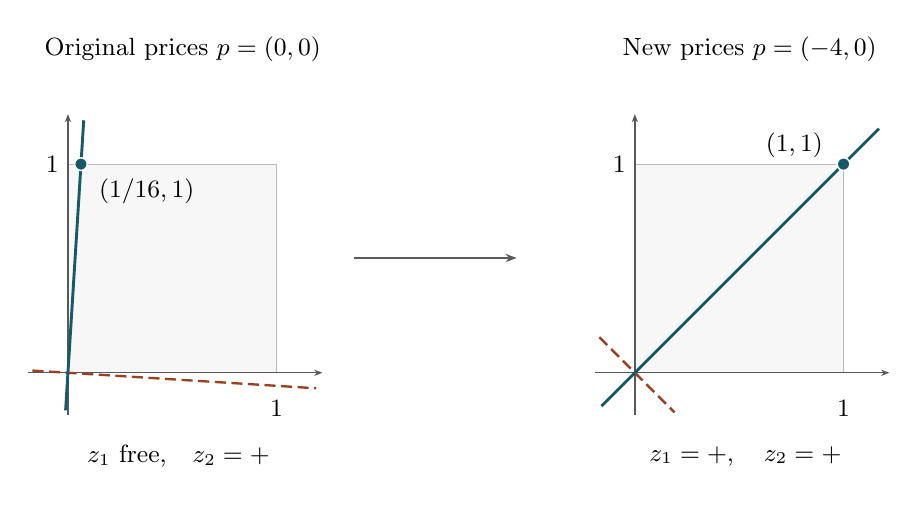
\begin{tikzpicture}[x=2.65cm,y=2.65cm,font=\small,
  primal/.style={lagoon,line width=1.05pt},
  dual/.style={ember,line width=.85pt,dash pattern=on 4pt off 2pt},
  axis/.style={-{Stealth[length=3pt]},line width=.45pt,black!65},
  marker/.style={fill=lagoon,draw=white,line width=.55pt}]
  \newcommand{\priceaxes}{%
    \fill[black!3] (0,0) rectangle (1,1);
    \draw[black!27,line width=.4pt] (0,1)--(1,1)--(1,0);
    \draw[axis] (-.19,0)--(1.22,0);
    \draw[axis] (0,-.2)--(0,1.24);
    \node[anchor=east,inner sep=2pt] at (-.015,1){\(1\)};
    \node[anchor=north,inner sep=2pt] at (1,-.105){\(1\)};
  }
  \begin{scope}
    \priceaxes
    \node at (.55,1.55){Original prices \(p=(0,0)\)};
    \draw[dual] (-.17,.010625)--(1.19,-.074375);
    \draw[primal] (-.01125,-.18)--(.075625,1.21);
    \path[marker] (.0625,1) circle[radius=2.3pt];
    \node[anchor=west,inner sep=2pt] at (.12,.87){\((1/16,1)\)};
    \node at (.53,-.40){\(z_1\) free,\quad \(z_2=+\)};
  \end{scope}
  \begin{scope}[xshift=7.2cm]
    \priceaxes
    \node at (.55,1.55){New prices \(p=(-4,0)\)};
    \draw[dual] (-.17,.17)--(.19,-.19);
    \draw[primal] (-.16,-.16)--(1.17,1.17);
    \path[marker] (1,1) circle[radius=2.3pt];
    \node[anchor=east,inner sep=2pt] at (.93,1.09){\((1,1)\)};
    \node at (.53,-.40){\(z_1=+,\quad z_2=+\)};
  \end{scope}
  \draw[-{Stealth[length=4pt]},black!65] (1.37,.55)--(2.15,.55);
\end{tikzpicture}
\caption{Making a small witness coordinate visible. The solid line is
the scaled primal space for \(C=\operatorname{span}\{(1/16,1)\}\), and
the dashed line is its orthogonal complement. The dot is the
nonnegative primal vector of sup norm one. Multiplying its first
coordinate by \(16\) and the corresponding dual coordinate by
\(1/16\) preserves orthogonality. At the new prices both coordinates
reach the visibility threshold \(1/2\), so both labels are forced.
Coordinates \(1\) and \(2\) are horizontal and vertical, respectively.}
\label{fig:scale}
\end{figure}


At a given \(p\), imagine a test that labels \(i\) with the correct
side whenever some scaled, normalized nonnegative vector has \(i\)th
entry at least \(1/2\). The other labels may be arbitrary. How could
these answers decide \emph{every} side? Fix a nonnegative circuit \(u\)
on side \(h\in\{-1,+1\}\). For each \(i\) in its support, the
\emph{slot} \(s=(i,h)\) records the coordinate and its side. Assign it
an integer \emph{demand}
\[
 a_s=\lfloor\log_2 u_i\rfloor+b_u,
\]
with a common shift \(b_u\) chosen so that all demands are positive.
At any slot maximizing \(a_s-hp_i\), the scaled entry is within a
factor of two of the largest scaled entry of \(u\). The label is
therefore correct at every such maximizer, even though the test
reveals neither the circuit nor the maximizing slots.

\begin{theorem}[Extremal prices]\label{thm:prices}
Let \(N,R\ge1\) be integers and let \(\Slots=[N]\times\{-1,+1\}\).
There is a deterministic algorithm that queries price vectors
\(p\in\QQ^N\), receives a label vector \(z\in\{-1,+1\}^N\) for each
query, and returns \(x\in\QQ^N\) with the following guarantee.

A hypothesis consists of a nonempty set \(S\subseteq\Slots\) and
integer demands \(a_s\in[-R,R]\) for \(s\in S\). Its surplus at
\(s=(i,h)\) is \(d_s(p)=a_s-hp_i\). Call the hypothesis
\emph{consistent} if at every query and answer \((p,z)\),
\[
   s=(i,h)\in S,\qquad
   d_s(p)=\max_{u\in S}d_u(p)\ge0
   \quad\Longrightarrow\quad z_i=h.
\]
For each consistent hypothesis the output meets all its demands,
that is, \(h x_i\ge a_s\) for every \(s=(i,h)\in S\).
The bit time, including all query and answer bits, is polynomial in
\(N\) and \(\log(R+1)\).
\end{theorem}

For the ideal test, every nonnegative circuit defines a consistent
hypothesis as soon as \(R\) bounds its demands. Since each coordinate
has a witness circuit and its demand is positive, the sign of \(x_i\)
gives its side. The prices returned by the theorem need only encode
these signs. The separate queries have already supplied the evidence.

\subsection{How to answer a price query}

Two numerical obstacles remain. A circuit can have entry ratios of
arbitrary magnitude, so the bound \(R\) from the ideal test can be
arbitrarily large at fixed dimension. Even when a rational price
\(p_i\) has few bits, the scaling factor \(2^{p_i}\) may require
prohibitively many bits to represent. The calibration procedure in
Theorem~\ref{thm:cal} gives the search a short description of the
geometry it needs. Figure~\ref{fig:architecture} shows how a query is
answered.

\begin{figure}[htbp]
\centering
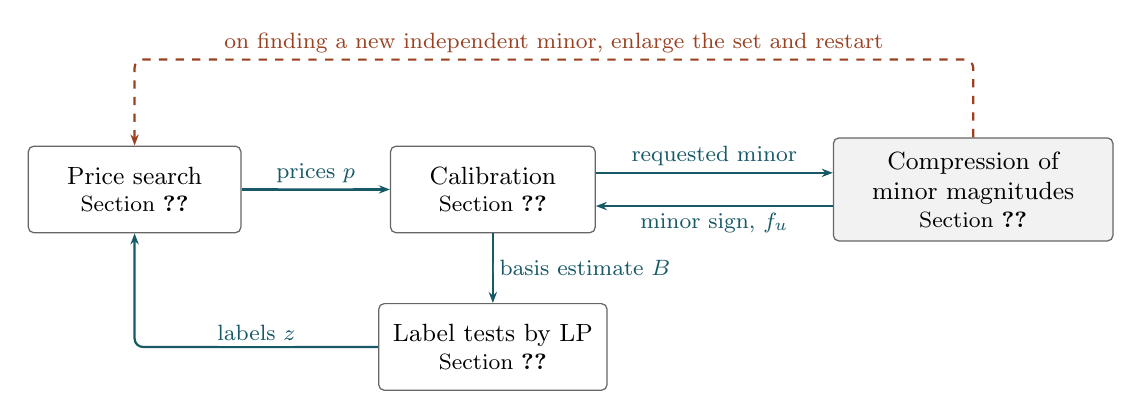
\begin{tikzpicture}[x=1cm,y=1cm,font=\small,
   operation/.style={draw=black!60,fill=white,line width=.45pt,
     rounded corners=2pt,align=center,inner sep=5pt,minimum height=1.1cm},
   data/.style={-{Stealth[length=4pt]},lagoon,line width=.8pt,
     rounded corners=3pt},
   again/.style={-{Stealth[length=4pt]},ember,dashed,line width=.8pt,
     rounded corners=3pt},
   msg/.style={font=\footnotesize,inner sep=2pt,fill=white}]
  \node[operation,minimum width=2.7cm] (learn) at (1.45,0)
    {Price search\\[-1pt] \footnotesize Section~\ref{sec:prices}};
  \node[operation,minimum width=2.6cm] (cal) at (6.0,0)
    {Calibration\\[-1pt] \footnotesize Section~\ref{sec:calibration}};
  \node[operation,minimum width=3.55cm,fill=black!5] (comp) at (12.1,0)
    {Compression of\\minor magnitudes\\[-1pt] \footnotesize Section~\ref{sec:compression}};
  \node[operation,minimum width=2.9cm] (labels) at (6.0,-2)
    {Label tests by LP\\[-1pt] \footnotesize Section~\ref{sec:lp}};
  \draw[data] (learn.east)--node[msg,midway,above]{prices \(p\)} (cal.west);
  \draw[data] ([yshift=6pt]cal.east)--
     node[msg,midway,above]{requested minor} ([yshift=6pt]comp.west);
  \draw[data] ([yshift=-6pt]comp.west)--
     node[msg,midway,below]{minor sign, \(f_u\)}
     ([yshift=-6pt]cal.east);
  \draw[data] (cal.south)--node[msg,midway,right]{basis estimate \(B\)} (labels.north);
  \draw[data] (labels.west)--node[msg,above,midway]{labels \(z\)}
      (1.45,-2)--(learn.south);
  \draw[again] (comp.north)--(12.1,1.65)--
      node[msg,midway,above]{on finding a new independent minor, enlarge the set and restart}
      (1.45,1.65)--(learn.north);
\end{tikzpicture}
\caption{Answering queries during a side decision. The shaded step uses the original scalar entries. For a nonzero minor
it supplies the sign and a short substitute \(f_u\) for the logarithm
of its magnitude. The other steps use rational data of polynomial bit
length. Each restart clears the price search and retains the enlarged
set of minor indices. Once the search finishes, the signs of its
returned prices give the sides.}
\label{fig:architecture}
\end{figure}


Apply calibration to a row basis \(B_0\) of \(W=C\times C^\perp\),
with one column for each slot. Between successive restarts, the
queries share a single assignment of positive integer demands to
every circuit of \(W\). The bit length of these demands is bounded by
a polynomial in the dimension and the chosen precision. At each
queried \(p\), calibration returns a rational matrix \(B\). For
the analysis there is a reciprocal diagonal scaling \(D\) with two
properties. First, \(B\) closely approximates a row basis of \(WD\)
in which each vector of sup norm one has bounded coefficients.
Second, every slot of maximum surplus for a circuit has scaled
entry of magnitude at least one third of its largest scaled entry.
One \(D\) works for all circuits at this query. Its entries may be
very large, but only \(B\) has to be computed.

To get labels from \(B\), solve an ordinary bit-polynomial LP for each
coordinate. Give \(i\) label \(+\) if a bounded row combination of
\(B\) is nearly nonnegative, stays in a bounded box and has
\((i,+)\) entry at least \(1/4\). Otherwise give it label \(-\).
The gap between \(1/3\) and \(1/4\) absorbs the approximation error.
Opposing slots cannot both pass. In the true scaled space every
vector \(v\) has \(\sum_i v_{i+}v_{i-}=0\) by orthogonality. If both
tests passed, the midpoint of two passing combinations would have
large entries in both slots and only tiny negative entries elsewhere,
making this sum bounded away from zero. Section~\ref{sec:lp} makes the
error bounds explicit. A circuit of \(C\) or \(C^\perp\) embeds in
\(W\) by zeros on the other side, so all witness circuits remain
consistent through the final uninterrupted run of the price search.

\paragraph{Why minors suffice.}
Elimination and the description of circuits use the same data.
Fix all but one column in a square minor of \(B_0\), then vary the
last column. The resulting determinants give a vector in the row
space. Taking the fixed columns to be preceding pivots gives the
next elimination row. Taking independent columns outside a circuit's
support gives that circuit up to scale. Consequently the magnitudes
needed to choose pivots and assign demands are governed by the same
numbers, the logarithms \(\ell_u\) of the absolute nonzero minors.

Calibration uses substitutes \(f_u\) of short bit length. They preserve
the signs, including zeros, of integer affine forms with bounded
coefficients in a slight perturbation of the logarithms. To see why
this suffices, choose a pivot using \(f_u\) and the queried prices.
Record, on a fine grid, the scaled log differences from this pivot
for the other entries. For tiny relative magnitudes only an upper
bound is needed. Requiring prices to reproduce these intervals gives
linear inequalities. Eliminating the prices leaves affine
inequalities in the log data with bounded integer coefficients.
They hold for \(f\), hence also for the perturbed logs. A common
price vector for the latter therefore exists. In the true geometry
it realizes the same normalized cofactor entries to the accuracy
needed for \(B\) and for the visibility bound
(Section~\ref{sec:calibration}).

\paragraph{Why few scales suffice.}
There may be exponentially many nonzero minors. Section~\ref{sec:compression}
extends Frank--Tardos rounding~\cite{FT} to requests for one minor at
a time. The reason this works is a counting argument. Suppose the
subset sums of \(k\) minor logarithms all differ by more than two.
The corresponding \(2^k\) products of minors then have magnitudes that
more than double in sorted order, so their \(2^{2^k}\) subset sums
are distinct. Yet each sum is the value of an integer polynomial in
the matrix entries, of bounded degree and coefficient size.
Counting these polynomials bounds \(k\) by a polynomial in the
dimensions.

The procedure keeps a set of minor indices with this separation
property for accurate proxies of the logs. Lattice reduction~\cite{LLL}
provides a sequence of scales for the set. On a request, the procedure
tries to express the new proxy in those scales using bounded integer
digits and a small remainder. Success gives a short substitute, and
all answers since the last restart extend to an assignment for every
nonzero minor. Failure proves the index can be added to the separated
set. The search then starts again with a larger set, which the
counting bound permits only polynomially many times. Comparisons
for extracting digits use ordinary arithmetic on the inputs.
Small logarithms can be approximated directly. When a comparison
involves an exceptionally large logarithm it can instead be decided
by comparing products of powers of minors. In that case the input
itself has enough bits, on rational data, to bound the bit length of
the powers.

Once the search returns all side signs, actual witnesses can be
recovered by testing which coordinates can be set to zero while
retaining a witness at the desired coordinate. At minimal support
the restricted space is a line. Solving on that line recovers the
witness in the original scale. Applying feasibility to the recession
and primal--dual optimality systems then gives the alternatives in
Theorem~\ref{thm:lp}.

\subsection{Learning all demands from extremal labels}

It remains to explain how Theorem~\ref{thm:prices} turns labels into
prices. First suppose we can afford one expert per hypothesis. Give
each expert an initial unit of wealth and let it bet on a slot of
greatest surplus, with the option of abstaining at utility zero.
Choose prices to minimize the wealth-weighted sum of maximum
utilities. At this minimum, bets on opposite signs of each
coordinate balance if ties are split suitably. Multiplying wealth
according to agreement with the labels can therefore keep total
wealth from increasing, even with ties resolved against each expert.
An expert for a consistent hypothesis never loses wealth. Whenever
any of its demands is unmet, every maximizing slot has a true label
and the expert's wealth grows by a fixed factor. This can happen only
logarithmically many times in the number of experts. A majority of
queries can thus meet each consistent hypothesis's demands, and
taking a coordinatewise median preserves each such bound. The choice
of prices is related to the balanced points of Chen, Li and
Yannakakis~\cite{CLY}.

The full pool is too large to process. An expert who guesses the
demands on just four slots, however, may miss the single largest
surplus and receive no useful label. The recursive search in
Section~\ref{sec:prices} amplifies the feedback, building on
Soleymani and Farina~\cite{SF} and on earlier algorithms for
games~\cite{OAIDe,OAIRa,OAITu}. From a proposal \(y\), make a child
call that returns prices \(x\). Use the sign of \(x_i-y_i\) as
feedback at \(y\), and query the label at \(x\) to break ties.
Suppose the child has brought every surplus down to a threshold
\(t'\ge0\). For any slot \(s=(i,h)\) with \(d_s(y)\ge t'\),
\[
 d_s(x)\le t'\le d_s(y)\qquad\Longrightarrow\qquad h x_i\ge h y_i.
\]
Even equality gives correct feedback, since that slot then maximizes
surplus at \(x\). A single child can therefore give correct feedback
on every slot above a common threshold.

The analysis assigns a weight distribution on slots and a threshold
to each node for each consistent hypothesis. If few slots by weight
violate the current threshold, the child retains it. When many
violate it, the child takes a higher threshold at a surplus quantile.
Success then gives correct feedback on an upper fraction of all
slots, which four sampled slots have a constant chance to hit.
Experts guess the threshold from the price history as well as the
four demands. A median combines the children, and increasing the
weight of persistently violated slots limits the necessary depth to
\(O(1+\log N)\).

Polynomial running time also requires controlling the number of
children. An expert invests a fraction of its wealth in a child
while using the rest to bet locally. A failed child must return enough
wealth to some experts to compensate for losses on its feedback.
This accounting allows a constant number of children below the root
and rules out failure at the root. Finally, experts guessing the same
four slots and the same threshold pivot can be grouped by their
at most five demand values. The regions on which those experts act
alike have fixed dimension, so their collective bets can be computed
in polynomial bit time.

\paragraph{Other uses of the price theorem.}
For monotone linear complementarity, the signs identify which member
of each complementary pair must vanish for a solution on the
selected support. A convex quadratic test supplies labels, after
which linear feasibility gives the solution
(Section~\ref{sec:quadratic}). For a contraction in the max norm, a
coordinate of greatest fixed-point error moves toward the fixed
point under the map. This gives extremal labels from function values
(Section~\ref{sec:contractions}). Discounted value equations for
turn-based games furnish piecewise-affine examples. Section~\ref{sec:games}
uses these equations together with LP policy evaluation to recover
exact values and strategies.

\section{Linear programming by pricing}\label{sec:lp}

For a subspace \(C\subseteq\RR^N\), consider the two nonnegative cones in
\(C\) and \(C^\perp\). At each coordinate \(i\), exactly one of these cones
contains a vector positive at \(i\). In the homogenized slack space of a
linear program, the two possibilities at the homogenizing coordinate
give a feasible point and a certificate of infeasibility, respectively.
We first determine which cone contains the witness, then recover the
witness itself with inclusion-minimal support.

Call \(C\) the positive side and \(C^\perp\) the negative side.
Orthogonality excludes simultaneous witnesses at \(i\). If the system
\(v\in C,\ v\ge e_i\) is infeasible, Farkas' lemma gives a nonnegative
vector in \(C^\perp\) positive at \(i\), proving that one side always
has a witness. Moreover, a witness \(u\) of inclusion-minimal support
is a circuit. If there were a second independent vector on its support
in the same subspace, a linear combination would give a nonzero
direction supported there and vanishing at \(i\). Move from \(u\)
along that direction, choosing the sign that decreases some entry,
until the first entry vanishes. This yields a witness with smaller
support. For the relation with elementary vectors and the classical
theorems of Minty and Tucker, see~\cite[Theorem~6 and its corollary]{Rock}
and~\cite{Tuc}.

\subsection{Reciprocal scaling and visibility}

To use Theorem~\ref{thm:prices}, we need a label at each coordinate of
each queried price vector. Scale coordinate \(i\) on the positive side
by a positive factor and on the negative side by its reciprocal. This
preserves orthogonality and can bring a small circuit entry into view.
The following theorem chooses the effective scaling for each query
and describes its effect using a rational matrix of short bit length.

Write \(\Slots=[N]\times\{-1,+1\}\) and abbreviate the slots
\((i,\pm1)\) by \(i\pm\). A \emph{reciprocal scaling} is a positive
diagonal matrix \(D\) on these slots with \(D_{i+}D_{i-}=1\) for all
\(i\). For row vectors, scaling acts by right multiplication. The
scale for a query \(p\) will make every slot maximizing surplus visible,
even when the factors \(2^{-p_i},2^{p_i}\) would be too costly to represent.

\begin{theorem}[Calibration]\label{thm:cal}
Given an ordered row basis \(B_0\) of a real subspace \(W\)
on the paired slots of \([N]\), \(N\ge1\), and an integer precision
parameter \(P\ge1\), there is a deterministic procedure answering
online price queries \(p\in\QQ^N\) by rational matrices \(B\).
On a query it may instead declare a restart.

At any time, all answers since the most recent restart, or since
initialization, admit the same assignment of demands. For each circuit
\(u\) of \(W\) the assignment gives an integer \(a_s\in[1,R]\) at each
slot \(s\) in its support.
For each such answer \(B\) at prices \(p\),
there is a reciprocal scaling \(D\) with the following properties.
\begin{itemize}
 \item \(B\) approximates a true row basis \(B_*=L B_0D\) of \(WD\)
 to within \(2^{-P}\) entrywise, with \(L\) lower triangular with
 positive diagonal. Entries of \(B_*\) have absolute value at most
 \(2\). Any vector in \(WD\) of sup norm one has row coefficients
 in this basis of absolute value at most \(2^{100N^2}\).
 \item For every circuit \(u\), at each slot \(s=(i,h)\) maximizing
 surplus \(a_s-hp_i\) on the support of \(u\),
 \[
       |(uD)_s|\ \ge\ \tfrac13\|uD\|_\infty .
 \]
\end{itemize}

The integer bound \(R=2^{\poly(N,P)}\) is available at initialization,
and the total number of restarts is polynomial in \(N,P\). The
procedure is strongly polynomial when the value of \(P\), the number
of queries, and the bit lengths of the prices count as additional
discrete input size. It returns the answers in explicit binary form.
\end{theorem}

The algorithm receives the approximate basis \(B\). The true basis
\(B_*\), the scaling \(D\), and the demands certify the properties of
that answer. The triangular factor \(L\) will also preserve the row
order and orientation needed in Section~\ref{sec:quadratic}.

\subsection{From approximate labels to exact witnesses}

Embed the two sides in \(W=C\times C^\perp\), with \(C\) on the positive
slots and \(C^\perp\) on the negative slots. A witness circuit of either
side is still a circuit in \(W\) after extension by zero on the other
side. The quadratic form
\[
 Q(y)=\sum_{i=1}^N y_{i+}y_{i-}
\]
vanishes on \(W\) and on every reciprocally scaled space \(WD\).
This identity lets us label a coordinate even though calibration returns
only an approximate basis.

\paragraph{Testing one side.}
Apply Theorem~\ref{thm:cal} to a row basis of \(W\), taking
\begin{equation}\label{eq:labelpars}
 H=2^{100N^2},\qquad \epsilon=H^{-10},\qquad 2^{-P}=H^{-100}.
\end{equation}
Run the algorithm of Theorem~\ref{thm:prices} with the resulting bound
\(R\). At each price query, request the calibrated basis. If calibration
declares a restart, begin a fresh price search, retaining the state of
the calibration procedure. Otherwise let \(B\) be the matrix returned.
Form the convex set
\begin{equation}\label{eq:box}
 \mathcal B(B)=\{y=\xi B:\|\xi\|_\infty\le H,\quad
                     -\epsilon\le y_s\le2\quad(s\in\Slots)\}.
\end{equation}
Give label \(+\) at \(i\) if some \(y\in\mathcal B(B)\) has
\(y_{i+}\ge1/4\), and give label \(-\) otherwise.
Each test is linear feasibility on explicit short rational data, so
ordinary bit-polynomial LP suffices~\cite{Khach,GLS}.

To see why testing the positive slot suffices, write a candidate
as \(y=\xi B\) and compare it with \(y_*=\xi B_*\) in the true
scaled space. There are at most \(2N\) rows, so
\(\|y-y_*\|_\infty\le 2NH2^{-P}<\epsilon^2\).
Since \(Q(y_*)=0\) and the entries of \(y\) belong to
\([-\epsilon,2]\), we have \(Q(y)\le5N\epsilon^2\le H^{-1}\).
The following observation will also apply in quadratic programming.

\begin{lemma}\label{lem:mid}
Let \(K\) be a convex set of vectors on the paired slots, with
\(-\epsilon\le y_s\le2\) and \(Q(y)\le H^{-1}\) for every \(y\in K\).
For each \(i\), at most one of its two slots attains \(1/4\) or more
anywhere in \(K\).
\end{lemma}
\begin{proof}
If a vector attaining the threshold exists at each slot, their
midpoint has both entries at least \((1/4-\epsilon)/2\ge1/10\).
Every other pair contributes at least \(-2\epsilon\). Thus the
midpoint belongs to \(K\) and has
\(Q\ge10^{-2}-2N\epsilon>H^{-1}\), a contradiction.
\end{proof}

\paragraph{Deciding all coordinates.}
In the final run between restarts, calibration supplies a common
assignment of positive demands to every circuit.
Fix a nonnegative circuit \(u\) and consider any query \(p\). If the
slot \(s=(i,h)\) maximizes the surplus of this circuit, its normalized
scaled vector
\[
 y_*=uD/\|uD\|_\infty=\xi B_*
\]
has \((y_*)_s\ge1/3\) and admits coefficients with
\(\|\xi\|_\infty\le H\). All entries of \(y_*\) lie in \([0,1]\).
The same approximation estimate shows that \(\xi B\) belongs to
\(\mathcal B(B)\) and attains at least \(1/4\) at \(s\). For \(h=+1\)
the positive test therefore succeeds. For \(h=-1\) Lemma~\ref{lem:mid}
forces the positive test to fail. In either case the returned label at
\(i\) equals \(h\).

Thus the slots and demands of each nonnegative circuit form a
consistent hypothesis for Theorem~\ref{thm:prices}. The returned
prices \(x\) satisfy \(hx_i\ge a_s\ge1\) at \emph{every} slot of that
circuit. Every coordinate has a witness circuit, so \(\sgn(x_i)\)
identifies the side of every coordinate. Calibration restarts only
polynomially often. In each run Theorem~\ref{thm:prices} bounds
the number of queries and their bit lengths by a polynomial in
\(N,\log(R+1)\). The calibrated answers and the rational label tests
then have strongly polynomial total cost by Theorem~\ref{thm:cal}.

\paragraph{Recovering one circuit.}
Fix a target coordinate \(i\) and take the subspace on its indicated
side. For each coordinate \(j\ne i\) in turn, tentatively impose
\(v_j=0\) on the current subspace. Keep the restriction exactly when
the side decision for this smaller subspace says it still contains
a nonnegative vector positive at \(i\). A rejected restriction can
never become feasible later, since each remaining step shrinks the
subspace. Consequently every final witness is positive on every
unrestricted coordinate. The direction argument at the start of this
section now shows that the final subspace is a line. Linear algebra
recovers its generator, oriented to be positive at \(i\), and hence
a witness circuit in the original subspace. At each trial we compute
a basis from the original input and the retained zero coordinates.
The bit bounds are given in Section~\ref{sec:arithmetic}.

\subsection{Certificates for a linear program}

\begin{proof}[Proof of Theorem~\ref{thm:lp}]
For \(Ax\le b\) use the homogenized slack space and its orthogonal
complement,
\[
 \begin{aligned}
 C      &=\{(\alpha b-Ax,\alpha): x\in\RR^n,\ \alpha\in\RR\},\\
 C^\perp&=\{(y,-b^\top y): A^\top y=0\}.
 \end{aligned}
\]
Recover a witness circuit at the last coordinate. On the positive
side, divide the witness by its last coordinate and solve for \(x\)
by linear algebra. This gives \(Ax\le b\). On the negative side,
the witness gives \(y\ge0\), \(A^\top y=0\), and \(b^\top y<0\).
The codimension of \(C^\perp\) is \(1+\rank A\). A circuit in a
space of codimension \(k\) has at most \(k+1\) entries in its
support, since its support indexes a minimally dependent set of
columns of a defining matrix. The last entry of this circuit is
positive, leaving at most \(1+\rank A\) entries for \(y\).

This also solves feasibility with both strict and weak inequalities.
Homogenize with a variable \(\alpha\), require \(\alpha\ge1\), and
require each slack belonging to a strict inequality to be at least
one. A solution of the original mixed system can be scaled to meet all
these lower bounds. Dividing by \(\alpha\) gives the converse.

For a feasible program, test \(Ar\le0,\ c^\top r>0\) by this
procedure. A solution, together with the feasible point already
found, certifies unboundedness. Otherwise LP duality gives finite
primal and dual optima with a common value \(v\). Strict
complementarity~\cite{GT} ensures that some optimal pair satisfies
\(b-Ax+y>0\). For completeness, take a coordinate \(i\) whose slack
is zero at every primal optimum. Maximize that slack subject to
\(Ax\le b\) and \(c^\top x\ge v\). Duality for this auxiliary
program, which has value zero, gives \(u\ge0\) and \(\lambda\ge0\)
with
\[
 A^\top(u+e_i)=\lambda c,\qquad b^\top(u+e_i)=\lambda v .
\]
If \(\lambda>0\), dividing \(u+e_i\) by \(\lambda\) gives a dual
optimum positive at \(i\). If \(\lambda=0\), adding \(u+e_i\) to
any dual optimum has the same effect. Averaging the primal witnesses
for the coordinates admitting positive slack, and the dual witnesses
for those with necessarily zero slack, gives a strictly complementary
pair. If one of these collections is empty, any optimum on that side
suffices.

The algorithm recovers the pair directly, without knowing \(v\).
Solve the single mixed linear feasibility problem
\[
 Ax\le b,\quad y\ge0,\quad A^\top y=c,\quad
 b^\top y=c^\top x,\quad b-Ax+y>0.
\]
The equality makes the duality gap \((b-Ax)^\top y\) zero. This
returns the optimal pair with the required strict complementarity.
\end{proof}

\subsection{Arithmetic and bit lengths}\label{sec:arithmetic}

The bounds used above apply to one uniform program for all input dimensions.
Our control operations on explicit strings (indices or
short rationals generated by the algorithm)
are charged full bit cost, and can use any polynomial-time
bit algorithm on strings of polynomial length in the dimension.
We take standard explicit input with dimensions and a nonzero end marker
(so size is at least the dimensions, also in the bit bounds).
To simulate the algorithms on the real machine of~\cite{BSS}, store
each explicit bit in a cell. Even sequential memory scans that
increment or reset indices and copy cells incur only polynomial
overhead. All polynomial bounds are fixed and effective. When such a
bound is used as an algorithmic parameter, one can fix it by
composing the estimates in the proof.
Logarithms are to base two unless indicated by \(\ln\).

We can implement all scalar arithmetic using pairs
\((u,v)\), meaning \(u/v\) (\(v>0\)),
and perform only ring operations and comparisons aside from
possible final divisions.
This representation admits two input conventions.
\begin{itemize}
  \item Input a scalar \(x\) directly, starting with \((x,1)\).
    Measure bit lengths on rational data by \emph{reduced} fractions
    (of the entries \(u,v\) themselves, and similarly for intermediates).
  \item Give each rational scalar as numerator and denominator
    (integer scalars). Compute with integer pairs and return the
    resulting unreduced pair for each output scalar.
    Measure bit lengths by the full sizes of these integers.
    This uses only the most restrictive division convention
    in~\cite[\S1.3]{GLS}.
    See also~\cite{DKNOV} for a discussion of arithmetic models.
\end{itemize}
These bounds give a polynomial-time Turing simulation. A simulation
may reduce fractions in the first model and store the integer pairs as given
in the second. Neither algorithm
itself uses fraction reduction in scalar arithmetic. Short rationals \emph{given or constructed in
bits} may be freely placed in scalar computations by setting up their
numerators and denominators bit by bit.

To cover both versions, on rational data take as a pair's log height
the log of the least bound on absolute numerators and denominator
for writing \(u,v\) with one positive denominator.
All results and intermediates must have log height polynomial
in total input length (including bit sizes of any input pairs).
The usual pair operations incur log height at most the sum for their
arguments plus one (take the product of their two common denominators),
including for cross-products when comparing.
This gives the bit bound for arithmetic by polynomial-size formulas
(size counting all leaf occurrences).

We use ordinary linear algebra on explicit real matrices.
We give the determinant routine explicitly because repeated unreduced
fraction arithmetic in elimination could increase the bit lengths
(see also~\cite[\S1.4]{GLS}).
Multiply the given \(k\times k\) matrix by the product \(D\)
of all pair-denominators \(v\), forming each new entry by multiplying its numerator
by all denominators except its own. Thus the resulting matrix is
\(M=D B\), where \(B\) denotes the input matrix. Compute \(k!\det M\)
by Newton's identities. If \(c_i\) is the coefficient of \(t^i\)
in \(\det(I+tM)\), the recurrence is
\[
 i!c_i=\sum_{j=1}^i (-1)^{j-1}
 \frac{(i-1)!}{(i-j)!}
 \big((i-j)!c_{i-j}\big)\tr(M^j),\qquad 1\le i\le k.
\]
Use these division-free ring operations (factorial ratios are
products) and return \((k!c_k,k!D^k)\).
On rational data all entries of \(M\) and \(D\) have
a common denominator \(U\) of polynomial bit length with
polynomial-bit numerators. The degree \(i\) results here
can use denominator \(U^i\), with polynomial-bit numerators
(by determinant expansion for the \(c_i\), and similarly for
matrix powers and then partial results in the recurrence).
The algorithm applies the recurrence to the scalar entries of \(M\)
using ring arithmetic. The common denominator \(U\) serves only to bound
reduced bit lengths in the first input model. In the integer-pair model
all entries of \(M\) are integers, so \(U=1\).

Use bordered minor tests to pivot for rank (an invertible minor of
order less than the matrix rank can be enlarged, by the Schur
complement), and Cramer's rule for solving and obtaining bases.
A fixed number of successive linear-algebra computations and
polynomial-size formulas therefore preserves polynomial bit length.
In witness recovery the number of coordinate restrictions can grow with
the dimension. Each basis there is computed from the original input and
the current list of zero coordinates, which keeps the number of successive
linear-algebra computations on the scalars bounded.

\paragraph{Ordered fields.}
For any fixed input shape, unroll the field algorithm to its uniform
step bound. Each computation branch and its output conditions can
be expressed in the language of ordered rings, with division by a
nonzero denominator expressed by multiplication. Tarski's transfer
principle thus gives correctness with the same step bound over every
real closed field. For an arbitrary ordered field, run the argument in
a real closure. All operations on inputs from the original field stay
in that field, so the same certificates are obtained there.

\section{Calibrating the geometry to prices}\label{sec:calibration}

Theorem~\ref{thm:cal} asks for two guarantees from one scaling.
Elimination must produce a basis with bounded entries and bounded
expansion coefficients for unit vectors, and every
circuit must have a large coordinate wherever its assigned surplus is
maximal. The same matrix minors govern both requirements. We first
express them as comparisons of minor magnitudes, then show how to make
these comparisons using only short rational data.

\subsection{Cofactors for elimination and for circuits}

Let \(B_0\) be the given ordered basis, with \(r\) rows. Index its
nonzero minors by their row and column sets \(u\), and write \(\ell_u\)
for the base-two logarithm of the absolute determinant. For a list
\(T\) of \(j-1\) distinct columns, \(1\le j\le r\), define a row
vector \(c\) by
\begin{equation}\label{eq:cofactor}
 c_s=\det B_0\big[[j],(T,s)\big].
\end{equation}
The entry vanishes when \(s\) repeats a column of \(T\). Expansion
along the last column expresses \(c\) as a combination of the first
\(j\) rows of \(B_0\). The coefficient on row \(j\) is
\(\det B_0[[j-1],T]\), with the empty determinant equal to one.

There are two uses for this formula. In elimination, \(T\) is the
list of earlier pivots. Its determinant is nonzero, so \(c\) supplies
the next elimination row, with zeros at all earlier pivots. For a
circuit, take \(j=r\). The vectors of \(W\) supported on that circuit
form a line, so the columns outside its support have rank \(r-1\).
Choosing \(r-1\) independent columns there gives a cofactor vector
that vanishes outside the circuit. It is nonzero because \(B_0\) has
rank \(r\), and hence represents the circuit up to a scalar.

Consider for the moment the reciprocal scaling
\(D(p)_{i,h}=2^{-hp_i}\). Given a cofactor list \(T\) and a slot
\(s=(i,h)\) on its support, let \(u(s)\) be the associated minor
index. For a vector \(y\) of values on the minor indices, set
\begin{equation}\label{eq:rho}
 \rho_s(y,p)=y_{u(s)}-hp_i,\qquad
 \rho_s(\ell,p)=\log |(cD(p))_s|.
\end{equation}
Consequently a maximizing slot is a largest entry in absolute value,
and the difference from that maximum gives the logarithm of a
normalized entry magnitude.

The algorithm makes the comparisons using short rational substitutes
\(f_u\) for the logs. These substitutes need not have the same
numerical size as the logs. What we require is that for each query
\(p\) there exist prices \(\widehat p\) at which the true normalized
entry magnitudes agree, to the requested absolute accuracy, with
those computed from \((f,p)\). One vector \(\widehat p\) must work for
all the cofactor rows at that query, including circuits on which the
algorithm never requests a minor. Our construction will prove
existence of \(\widehat p\) by projecting a system of linear
inequalities.

\subsection{Linear types and online compression}

For two real vectors \(y,y'\) on the same finite index set, write
\(y\sim_M y'\) when every integer affine form of coefficient
\(1\)-norm at most \(M\), including its constant, has the same sign
in \(\{-1,0,1\}\) on \(y\) and \(y'\). This agreement of linear
types lets us transfer feasibility from one parameter vector to the
other. Compare the use of Frank--Tardos rounding in
\cite[Lemma~(6.6.1)]{GLS}.

\begin{lemma}[Projection]\label{lem:projection}
Consider a finite system of linear inequalities, strict or weak,
in \(k\) real unknowns and additional parameters \(y\).
Let all its affine forms have integer coefficients and
coefficient \(1\)-norm (including constant) at most \(A\), where \(A\ge2\).
Then feasibility is the same at any two parameter
vectors with \(y\sim_M y'\), where
\(M=(k+1) A^{k+1}\).

If there are no parameters and the system is feasible,
it has a solution with both a common positive denominator and the absolute
numerators at most \((A+1)^{k+1}\).
\end{lemma}
\begin{proof}
Fix the parameters. Give every strict inequality a common additional
margin \(\delta\) and write the resulting inequalities weakly. The
original system is feasible precisely when this weak system is
feasible for some \(\delta>0\). For fixed \(\delta\), Farkas' lemma
reduces feasibility to testing nonnegative combinations of the
inequalities that eliminate the \(k\) unknowns. It suffices to test
the extreme rays of this cone of multipliers.

On the support of an extreme ray the multiplier kernel has dimension
one. Its support thus has size at most \(k+1\), and subdeterminants
give an integral generator whose entries are at most \(A^k\) by
Hadamard's inequality. Each resulting affine form on the parameters,
with \(\delta\) set to zero, has coefficient norm at most
\((k+1)A^{k+1}\). Require the projected inequality to be strict if a
strict input inequality has a positive multiplier, and weak otherwise.
These conditions are necessary. They are also sufficient, since the
cone has finitely many extreme rays and one sufficiently small
\(\delta>0\) preserves every margin required by a strict combination.
Agreement of linear types preserves all these tests.

For the second assertion, let \(\delta\) be a new unknown and add
\(0\le\delta\le1\) to the system with margins. Intersect with a
closed orthant containing a solution with \(\delta>0\).
The new polyhedron is pointed and has a vertex maximizing \(\delta\).
Its constraint rows, with constants, have coefficient \(1\)-norm at
most \(A+1\). Cramer's rule and Hadamard's inequality now give the
claimed common denominator and numerator bounds.
\end{proof}

The next theorem, proved in Section~\ref{sec:compression}, furnishes
substitutes that agree in linear type with a small perturbation of
the true logs. A price query will use only the entries requested
during elimination. The guarantee for all the remaining minors is
what makes the conclusion about unseen circuits possible.

\begin{theorem}[Online compression]\label{thm:compression}
Given an \(r\times d\) real matrix (\(0\le r\le d\), \(d\ge1\))
and \(K\ge1\) an integer,
index its nonzero minors by \(u\) (specifying row and column sets)
and let
\(\ell_u\) be the base-two logarithm of their absolute values.
There is a deterministic procedure that, on request of an
individual index \(u\), supplies a rational \(f_u\)
or declares a restart.

At any time the answers since the most recent restart (if no restart,
all answers) admit a common assignment \(f\) of rationals to
\emph{all} the indices with a common positive denominator and absolute
numerators each bounded by \(F=2^{\poly(d,K)}\), such that
\begin{equation}\label{eq:compress}
 f\sim_{2^K} g\quad\text{for some }g\text{ with }
 \|g-\ell\|_\infty\le2^{-K}.
\end{equation}
The total number of restarts is bounded by a polynomial in \(d\).
Initialization and each request (including responses with explicit
bits or restarts) take strongly polynomial time,
counting the value of \(K\) as additional input size. The integer bound \(F\)
is available at initialization.
\end{theorem}

\subsection{The common lift}

For \(P\) in Theorem~\ref{thm:cal}, set
\[
 E=P+6,\qquad e=2^{-E},\qquad A=(E+5)2^E
\]
and take \(K\) least with \(2^K\ge(N+1)A^{N+1}\).
Fix price data \(p\) and assignments \(f,g\) for \(B_0\) as in
\eqref{eq:compress}. We encode the normalized cofactor magnitudes at
\((f,p)\) as follows. For each nonzero cofactor vector take the slot
\(t\) maximizing \(\rho_t(f,p)\), using a fixed tie rule. For each
slot \(s\) on the same support write
\[
 w=\rho_s(f,p)-\rho_t(f,p)\le0,\qquad
 \Delta=\rho_s(y,\widehat p)-\rho_t(y,\widehat p).
\]
In \(\Delta\) the vector \(y\) is the parameter and the \(N\) components
of \(\widehat p\) are the unknowns. Impose
\[
 \begin{cases}
 e\lfloor w/e\rfloor\le\Delta\le e\lceil w/e\rceil,
      & w\ge-E,\\
 \Delta\le-E, & w<-E.
 \end{cases}
\]
For a ratio smaller than \(2^{-E}\) it suffices to preserve that upper
bound. Ratios above the cutoff need only one grid cell to specify
their log. All constraints hold at \((y,\widehat p)=(f,p)\).
Multiplying by \(2^E\) gives integer forms of coefficient norm at
most \(A\), independent of the bit lengths of the original prices
and the proxies. Lemma~\ref{lem:projection} therefore gives a solution
\(\widehat p\) at \(y=g\), since \(f\sim_{2^K}g\). The system
includes every cofactor list, so the solution is a single price vector
shared by all of them. The algorithm never forms this system.

Replacing \(g\) by the true log vector \(\ell\) changes each
difference by at most \(2\cdot2^{-K}\le2e\). Thus at the lifted
prices the true difference is within \(3e\) of \(w\) for
\(w\ge-E\), and at most \(-E+2e\) for \(w<-E\). Taking
\(D=D(\widehat p)\) yields
\begin{equation}\label{eq:pivot-estimate}
 \left|\frac{|(cD)_s|}{|(cD)_t|}-2^w\right|\le8e.
\end{equation}
In the first case this follows from the mean value theorem applied to
\(2^x\) for \(x\le3e\). In the second, both magnitudes are at most
\(2^{-E+2e}\).

\subsection{The calibration procedure}

Use Theorem~\ref{thm:compression}
on \(B_0\), with \(K\) as just specified. Take \(R=4F\).
To answer a price query \(p\), grow a sequence of pivot slots \(T\), starting empty.
At row \(j=1,\ldots,r\), take the cofactor vector with
\(T\) consisting of the previous pivots.
To see there will be a pivot available, recall that this vector \(c\)
is in the span of the first \(j\) rows. Its coefficient on original row \(j\) is \(d_{j-1}=\det B_0[[j-1],T]\), nonzero
by construction (\(d_0=1\)). Thus \(c\ne0\).
Request \(f\) values for all its nonzero entries.
If a restart occurs, abandon the query with that report.
Otherwise compute the row as follows.
\begin{itemize}
 \item As pivot at this row take slot \(t\) maximizing
 \(\rho_s(f,p)\) on the support, breaking ties by the rule fixed above.
 This gives \(d_j=c_t\ne0\) for the next step.
 \item For row \(j\) of the answer \(B\),
 keep zeros, and at each supported slot \(s\) put a rational
 within \(e\) of
 \[
    \sgn(d_{j-1}c_s)\cdot 2^{\rho_s(f,p)-\rho_t(f,p)}.
 \]
\end{itemize}
One query visits at most \(r\) cofactor rows and requests at most
\(2Nr\) minor proxies. Signs and zeros use minors of the original
matrix, computed as in Section~\ref{sec:arithmetic}.
Theorem~\ref{thm:compression} bounds the cost of the requests and
the total number of restarts.
The rational approximations take polynomial bit time.
For exponents below \(-E\), use zero.
Otherwise, split off the integer power, leaving \(2^q\) with
\(0\le q<1\).
Use \(\ln 2=\sum_{j\ge1}2^{-j}/j\) and then the series for
\(\exp(q\ln 2)\), e.g., through \(E+10\) in each,
by geometric tail bounds.

\begin{proof}[Completion of the proof of Theorem~\ref{thm:cal} given Theorem~\ref{thm:compression}]
Fix any uninterrupted sequence of answers from initialization or the
last restart up to the present time. Theorem~\ref{thm:compression}
extends all the returned proxies to one vector \(f\). For each query
in the sequence choose the scaling \(D\) from its common lift.
For row \(j\) of \(B_*\), use the corresponding \(cD\)
with sign adjusted by \(\sgn(d_{j-1})\)
and scaled to absolute entry one at the pivot.
Thus it now has a positive coefficient on row \(j\)
of \(B_0D\), giving \(B_*=L B_0D\)
with \(L\) as required.
By~\eqref{eq:pivot-estimate}, \(B\) is within \(9e\le2^{-P}\)
entrywise, and \(B_*\)
has entries bounded by two in absolute value.
Any vector of sup norm one in \(WD\)
can be expanded with coefficient on row \(j\)
bounded by \(3^{j-1}\le2^{100N^2}\)
in absolute value. Indeed, subtract row multiples in pivot order.
The pivot entry has magnitude one, so a residual of norm \(M\) requires
a coefficient of magnitude at most \(M\). The row itself has norm at
most two, leaving a residual of norm at most \(3M\).

For each circuit choose one cofactor representative and assign demands
\[
 a_s = 1+F+\lfloor f_{u(s)}\rfloor
\]
on its support. Since \(|f_{u(s)}|\le F\), these demands belong to
\([1,1+2F]\subseteq[1,R]\). They use the same \(f\) at every query in
the sequence.
Fix a circuit, with \(t\) as in the common lift
(so maximizing \(\rho_s(f,p)\) for this representative).
If \(s=(i,h)\) maximizes surplus \(a_s-hp_i\), then
\(w=\rho_s(f,p)-\rho_t(f,p)>-1\),
by the bound of one on rounding loss.
So in the common lift,
\(\rho_s(\ell,\widehat p)-\rho_t(\ell,\widehat p)\)
is greater than \(-1-3e\).
At any slot on this support, the true scaled log difference
from \(t\) is at most \(3e\).
Thus after scaling the circuit by \(D\), the entry at \(s\)
has magnitude at least
\(2^{-1-6e}\ge1/3\) times the sup norm.
\end{proof}

\section{Logarithmic compression on demand}\label{sec:compression}

Calibration requests the sizes of particular minors as it chooses pivots.
The choices must also be consistent with minors that never occur in a
pivot calculation, since such minors can enter a circuit. This is the
extension requirement in Theorem~\ref{thm:compression}. Write \(\ell_u\)
for the base-two logarithm of the magnitude of a nonzero minor. We seek
short rational answers to individual requests that extend to a vector
of the same linear type as a small perturbation of \(\ell\).

The procedure learns a set \(J\) of minor indices. Between restarts it
uses the logarithms at these indices to set common scales for all its
answers. A failure to represent a requested logarithm at those scales
enlarges \(J\). The bound on the number of restarts comes from the fact
that products of minors are polynomials of bounded degree in the same
matrix entries.

Throughout, an integer is \emph{short} if its bit length is polynomial
in \(d,K\). Fix
\[
 D=(d+1)^6,\qquad
 \eta^{-1}=\text{the least power of two at least }4D\cdot2^K .
\]
We first work with fixed proxies \(v_u\) satisfying
\(|v_u-\ell_u|\le\eta\) and access to the signs of integer affine
forms in these proxies. The final subsection constructs proxies for
which the required sign tests can be implemented in the arithmetic
model of Section~\ref{sec:arithmetic}.

\subsection{A bound on independent logarithms}

Call a set \(I\) of minor indices \emph{dissociated} if the subset sums
of \((v_u)_{u\in I}\) are pairwise at distance greater than two.
Equivalently, every nonzero coefficient vector in
\(\{-1,0,1\}^I\) gives a sum of absolute value greater than two.
This is a version with tolerance of the usual additive notion
\cite{LY}. If \(I\) is maximal, every proxy is within two of a signed
subset sum on \(I\). Indeed, for an index outside \(I\), any relation
preventing its addition must have coefficient \(+1\) or \(-1\) on the
new index.

\begin{lemma}\label{lem:dissociated}
Every dissociated set has size less than \(D\).
\end{lemma}
\begin{proof}
Suppose there is a dissociated set of size \(D\). The logarithms of
the magnitudes of its \(2^D\) subset products of signed minors differ by more
than \(2-D\eta>1\). In increasing order of magnitude each product
therefore has magnitude greater than the sum of all preceding
magnitudes. It follows that all \(2^{2^D}\) subset sums of these
products are distinct at the input matrix. Two unequal subsets
differ at a largest product, whose contribution survives cancellation.

These sums are consequently distinct integer polynomials in the
at most \(d^2\) matrix entries. Each has degree at most \(dD\) and
coefficients of absolute value at most \(2^D(d!)^D\), by the
determinant expansion. Counting possible coefficients at each
monomial gives
\[
 2^{2^D}\le
 \big(1+2^{D+1}(d!)^D\big)^{(dD+1)^{d^2}}.
\]
Two logarithms yield
\(D\le d^2\log(dD+1)+\log(2+D(1+d^2))
\le(7d^2+8)\log(d+1)\), contradicting \(D=(d+1)^6\).
\end{proof}

Goemans's bound on geometrically decreasing sequences of small integer
combinations uses a related counting argument
\cite[Lemma~3.5 in the preprint]{Newton}, attributed there via
Radzik~\cite{Rad}. Here the integer combinations are products of
minors expanded in monomials. Counting subset sums brings the
number of monomials into the dissociation bound only logarithmically.

\subsection{Extending partial answers}

Let \(S\) contain the indices answered since the last restart. To
certify answers on \(S\), we shall enforce agreement of linear type
at a larger coefficient bound \(M\) on \(S\) alone. Lemma~\ref{lem:extend}
shows why this suffices. A maximal dissociated set expresses all the
missing logarithms, to within a rounded offset, in fewer than \(D\)
variables. Projecting out these variables determines \(M\).

\begin{lemma}[Extension]\label{lem:extend}
Set
\[
 A=2^K(D+4)/\eta,\qquad M=(D+1)A^{D+1}.
\]
Suppose on a subset \(S\) of the indices we have
\begin{equation}\label{eq:answered}
 f_S\sim_M g_S,\qquad \|g_S-v_S\|_\infty\le\eta ,
\end{equation}
where \(f_S\) has a short common denominator and short numerators.
Then \(f_S,g_S\) extend to vectors \(f,g\) satisfying
\eqref{eq:compress} on all the minor indices. The vector \(f\) again
has a short common denominator and short numerators.
\end{lemma}
\begin{proof}
Choose a maximal dissociated set \(I\). For every \(u\notin S\),
write \(v_u\) as a signed subset sum on \(I\) plus an offset in
\([-2,2]\). Round the offset to the \(\eta\)-grid, and let \(h_u(x)\)
be the resulting affine form in \(x\in\RR^I\). Set
\(g_u=h_u(v_I)\). On \(S\) and its complement alike,
\(|g_u-\ell_u|\le 2\eta\le2^{-K}\).

Now impose the sign conditions
\[
  \big(y_S,\,(h_u(x))_{u\notin S}\big)\sim_{2^K}g .
\]
Here \(y_S\) is a parameter and \(x\) is an independent variable,
even when \(I\) meets \(S\). Write each sign as a strict inequality or
as two weak inequalities in the zero case. After clearing the grid
denominator, each row has integer coefficients of total absolute
value at most \(A\). For \(y_S=g_S\) we have the solution \(x=v_I\).
Since \(|I|<D\) by Lemma~\ref{lem:dissociated} and \(f_S\sim_M g_S\),
Lemma~\ref{lem:projection} gives a solution also at \(y_S=f_S\).

If \(U\) bounds the common denominator and the absolute numerators
of \(f_S\), the rows after substitution and clearing that denominator
have coefficient norm at most \(AU\). The second assertion of
Lemma~\ref{lem:projection} supplies \(x\) with a common denominator
and absolute numerators at most \((AU+1)^{D+1}\). Set \(f_u=h_u(x)\)
for \(u\notin S\). The product of the two common denominators and
\(1/\eta\) works for the whole vector. Both it and the absolute
numerators are bounded by \((D+2)(AU+1)^{D+1}U/\eta\).
\end{proof}

\subsection{Extracting common scales}

The maximal set \(I\) in Lemma~\ref{lem:extend} serves only to prove
existence. The procedure maintains its own dissociated set \(J\),
starting with the empty set. To decide whether it can answer a
request, it needs a test that succeeds on every proxy within two of
a signed subset sum on \(J\). Enumerating those sums would cost
exponential time. Instead we expand \(v_J\) at a sequence of common
scales. At each scale the vector of digits is integral and the
remaining error is a small fraction of the scale. This is the
simultaneous approximation step of Frank--Tardos rounding~\cite{FT}.

\begin{lemma}\label{lem:peel}
Let \(w\in\RR^m\), and fix integers \(\epsilon^{-1}\ge2\) and
\(H\ge0\). Put \(C=2^{m(m+1)}(2/\epsilon)^{m+1}\).
Given the signs of integer-coefficient affine forms on \(w\), one
can find integer vectors \(z_1,\ldots,z_p\) and positive scales
\(\lambda_1,\ldots,\lambda_p\), represented by rational linear forms
on \(w\), such that
\[
 \begin{aligned}
 &p\le m,\qquad \|z_j\|_\infty\le C,\qquad \lambda_j>H/C,\\
 &\left\|w-\sum_{i=1}^j\lambda_i z_i\right\|_\infty\le\epsilon\lambda_j
       \quad (1\le j\le p),\qquad
   \left\|w-\sum_{i=1}^p\lambda_i z_i\right\|_\infty\le H .
 \end{aligned}
\]
Counting each sign query as one operation, the bit time and the
lengths of all queries and outputs are polynomial in \(m\) and the
bit lengths of \(\epsilon^{-1},H\).
\end{lemma}
\begin{proof}
Start with remainder \(w'=w\). If \(X=\|w'\|_\infty>H\), use binary
search to find a rational vector \(u\) within \(\epsilon/(2C)\) of
\(w'/X\) in each coordinate. Consider the lattice of vectors
\((qu-z,q/C)\) for integral \(q,z\), of determinant \(1/C\).
Lattice reduction~\cite{LLL}, as in~\cite[Theorem~(5.3.19)]{GLS},
produces in polynomial bit time a nonzero vector of Euclidean norm
at most \(2^{m/2}C^{-1/(m+1)}\le\epsilon/2\). Such a vector must
have \(q\ne0\), since a nonzero integer vector has length at least
one. Choose its sign to give \(1\le q\le C\). Then
\[
 \|q w'/X-z\|_\infty\le\epsilon ,\qquad \|z\|_\infty\le q.
\]
For the second bound use integrality and \(\epsilon<1\).

Take \(\lambda=X/q>H/C\) and replace \(w'\) by \(w'-\lambda z\).
The new remainder has norm at most \(\epsilon\lambda\). At a zero
coordinate the digit is zero. At a coordinate attaining \(X\) in
absolute value the digit equals \(+q\) or \(-q\), so that coordinate
now vanishes as well. Thus at most \(m\) steps are needed to reach
residual norm at most \(H\). For \(m=0\) the expansion is empty.

Each comparison for the binary search can be made after multiplying
by \(X>0\). At every stage \(X\) is a signed coordinate of the
remainder, chosen by comparisons, so both the remainders and the
scales are rational linear forms in the original \(w\). A step
multiplies their common denominator by at most \(q\) and increases
the maximum absolute numerator by at most a factor \(2C\). Clearing
these denominators in the comparisons, including those on the
\(\epsilon/(2C)\)-grid, gives sign queries of the asserted length.
\end{proof}

For a homogeneous form, a nonzero integer digit contributes at least
one whole scale. Choosing the residual small compared with that scale
lets the first nonzero digit determine the sign. We record the usual
Frank--Tardos consequence used to round offsets in
Section~\ref{sec:contractions} and, through that computation, to
solve games in Section~\ref{sec:games}.

\begin{lemma}\label{lem:ft}
Given \(w\in\RR^m\) and an integer \(M\ge1\), one can find an integer
vector preserving the sign on \(w\) of every homogeneous linear form
with integer coefficients of \(1\)-norm at most \(M\). The procedure
is strongly polynomial with the bit length of \(M\) counted as
additional input size, and returns the entries in bits.
\end{lemma}
\begin{proof}
Apply Lemma~\ref{lem:peel} with \(\epsilon=1/(2M)\) and \(H=0\)
(cf.\ \cite[Theorem~(6.2.13)]{GLS}). For a form whose first nonzero
digit occurs on \(z_j\), the remaining contribution has magnitude
at most \(M\epsilon\lambda_j<\lambda_j\). A form vanishing on every
digit also vanishes on \(w\), since the final remainder is zero.
Consequently the integer vector
\(\sum_{j=1}^p(2CM+1)^{p-j}z_j\) has the required signs. Its first
nonzero digit dominates the geometric sum of all later digits,
whose evaluations have magnitude at most \(CM\) each. The short
linear forms queried in Lemma~\ref{lem:peel} can be evaluated as in
Section~\ref{sec:arithmetic}.
\end{proof}

For affine forms, append a coordinate equal to one before applying
Lemma~\ref{lem:ft}. Its rounded value is positive by sign agreement.
Dividing the rounded vector by that value preserves the homogeneous
signs and restores the last coordinate to one.

\subsection{Answering a request}

Start each sequence of requests by applying Lemma~\ref{lem:peel} to
\(v_J\). Use \(M\) from Lemma~\ref{lem:extend} and set
\[
 m=|J|,\qquad \epsilon^{-1}=100(m+1)M,\qquad H=100MC ,
\]
where \(C\) is determined by \(m,\epsilon\) in Lemma~\ref{lem:peel}.
All extracted scales \(\lambda_j\) exceed \(100M\). They remain fixed
throughout the sequence.

For a request at \(u\), look for integer digits \(b_{u1},\ldots,b_{up}\)
of magnitude at most \(mC\) satisfying
\begin{equation}\label{eq:request}
 \begin{aligned}
 \left|v_u-\sum_{i=1}^j\lambda_i b_{ui}\right|
       &\le\frac{\lambda_j}{10M} && (1\le j\le p),\\
 \left|v_u-\sum_{i=1}^p\lambda_i b_{ui}\right|
       &\le mH+2 .
 \end{aligned}
\end{equation}
Once the previous digits are fixed, the permitted interval for
\(b_{uj}\) has length \(1/(5M)<1\). Binary search therefore finds the
unique digit or detects failure. Check the last residual bound even if
there are no digits.

\paragraph{A failed request enlarges the dissociated set.}
If \(v_u\) lies within two of a signed subset sum on \(J\), take
the same signed sum of the digit vectors of \(v_J\) at each scale.
This gives digits of magnitude at most \(mC\) with residuals at most
\(m\epsilon\lambda_j+2\le\lambda_j/(10M)\) at position \(j\)
and at most \(mH+2\) at the end. Thus failure implies that \(u\)
lies outside \(J\) and that \(J\cup\{u\}\) is dissociated.
In that case retain the enlarged set, discard the expansion and
previous answers, and declare a restart. Each restart increases
\(|J|\) by one, so Lemma~\ref{lem:dissociated} bounds the total
number by \(D-1\).

\paragraph{A successful request gives a short answer.}
Round the final residual down to the \(\eta\)-grid by binary search,
obtaining \(e_u\) with \(|e_u|\le mH+2\) and error at most \(\eta\).
For \(B=10M(mH+3)\), return \(f_u\) and define its comparison value
\(g_u\) by
\[
 f_u=\sum_{j=1}^p B^{p+1-j}b_{uj}+e_u,\qquad
 g_u=\sum_{j=1}^p\lambda_j b_{uj}+e_u .
\]
Replacing the true scales by powers of \(B\) makes \(f_u\) rational
with common denominator \(1/\eta\) and absolute numerator at most
\(B^{p+2}/\eta\). Retaining the true scales in \(g_u\) gives
\(|g_u-v_u|\le\eta\).

To verify \(f_S\sim_M g_S\), write an integer affine form of norm at
most \(M\) as \(a_0+\sum_{u\in S}a_u x_u\). At position \(j\), its
combined digit is the integer \(\sum_{u\in S}a_u b_{uj}\). If all
combined digits vanish, the two evaluations equal
\(a_0+\sum_{u\in S}a_u e_u\). Otherwise let \(j\) be the first
nonzero combined digit. For \(g_S\), the magnitude contributed
after position \(j\), including the constant term, is bounded by
\[
 M\max\{\lambda_j/(10M)+\eta,1\}<\lambda_j
\]
by \eqref{eq:request} and the rounding error. For \(f_S\), each later
combined digit and the final affine term in \(e\) have magnitude at
most \(B/10\). Their geometric sum is smaller than \(B^{p+1-j}\).
The digit at \(j\) therefore determines both signs. The answers made
in this sequence satisfy \eqref{eq:answered}, and
Lemma~\ref{lem:extend} extends them to all minor indices.

Only \(J\) and its expansion are needed to answer the next request.
The comparisons in \eqref{eq:request} involve at most \(m+1\)
proxies. The product of the denominators \(q\) in Lemma~\ref{lem:peel}
clears coefficients in the scales, and a further factor \(10M/\eta\)
clears the residual and grid comparisons. All these integers
are short since \(p\le m<D\).
Thus initialization and each request require polynomial bit time with
sign access. A uniform integer bound \(F\) for Theorem~\ref{thm:compression}
is available at initialization by using \(U=B^{p+2}/\eta\) in
Lemma~\ref{lem:extend} and taking the largest bound over
\(0\le p\le m<D\).

\subsection{Implementing the sign tests}

A sign test on exact logarithms amounts to comparing a product of
powers of minors with a power of two. An exponent can have short bit
length and still produce very large rational intermediates. We use
rounded logarithms whenever their magnitudes are small. A large
logarithm, when it occurs, certifies that the rational input itself
has sufficient bit length for the power comparison.

Before defining the proxies, fix a short power of two \(T\) such
that every integer sign query used above has coefficient \(1\)-norm
at most \(T\eta\). This bound is uniform over choices of the proxies.
For example, the common denominators and absolute numerators for the
scale coefficients are bounded by \((2C)^m\), and the other
coefficients in the queries were bounded above in terms of \(d,K\).
These estimates allow \(T\) to be fixed for the worst case \(m<D\).

\paragraph{Determining the proxy.}
For each minor needed in a comparison, compute its absolute value
and invert it if necessary to obtain \(z_0=2^{|\ell_u|}\ge1\).
Compute powers \(2^k\) by squaring for \(k=1,2,4,\ldots,T\), stopping
at the first \(k\) for which \(z_0<2^k\). If no test succeeds then
\(|\ell_u|\ge T\) and we take \(v_u=\ell_u\), represented by the
minor itself. Otherwise binary search using powers of two supplies
the integer part of \(\log z_0\). The scalar powers computed in these
tests have exponents at most \(\max\{1,2|\ell_u|\}\). On rational
data this is polynomial in the input length by the determinant bound
of Section~\ref{sec:arithmetic}. The operation count is polynomial
in \(d,K\), since \(T\) is short.

After removing that integer power of two, the remaining factor
\(z\) lies in \([1,2)\). Compute the first \(\log(1/\eta)+6\) terms of
\[
 \ln z=\sum_{j\ge1}\frac{(1-1/z)^j}{j}
\]
and divide by the corresponding partial sum at two. Both series
tails admit a geometric bound, and the partial sum at two is at
least \(1/2\), so the quotient approximates \(\log z\) to error at
most \(\eta/4\). Use binary search to round to the nearest point of
the \(\eta\)-grid, breaking ties deterministically. Restoring the
integer part and sign produces explicit bits for a proxy within
\(\eta\) of \(\ell_u\). The fractional-part computation uses
polynomial-size formulas in \(z\) and short constants, and needs
only comparisons to perform the rounding.

\paragraph{Evaluating an affine form.}
If every participating minor has \(|\ell_u|<T\), evaluate the query
on the explicit proxy bits. Otherwise substitute the rounded proxies
and multiply by \(1/\eta\). The result is an integer constant plus
an integer combination of true logarithms. The constant and each
coefficient have magnitude at most \(2T^2\), by the norm bound
\(T\eta\) on the original form. Exponentiation to base two reduces
the sign test to comparing a product of integer powers of two and
of absolute minor values with one.

Binary powering gives a polynomial operation count in \(d,K\).
For rational data in this branch, some \(|\ell_u|\ge T\), so the
determinant bound puts \(T\) itself within a polynomial in total
input length. Each powering here could therefore be expanded into a
formula with polynomially many leaves in that length, proving the
required bound on intermediate log heights in both arithmetic
conventions of Section~\ref{sec:arithmetic}. Each query uses the
input matrix and short discrete data afresh. This proves
Theorem~\ref{thm:compression} and finishes the proof of
Theorem~\ref{thm:cal}.

\begin{remark}
The dissociation bound uses only the number of input variables, the
degree, and the coefficient \(1\)-norm of the minor polynomials.
The same compression procedure applies to any family of nonzero
values of integer polynomials in at most \(d^2\) scalar inputs whose
degrees are at most \(d\) and coefficient \(1\)-norms at most \(d!\).
It suffices that the indices are short and that each evaluation has
a deterministic strongly polynomial implementation in the chosen
arithmetic convention.
\end{remark}

\section{Learning from extremal prices}\label{sec:prices}

In the LP algorithm, a query chooses scales for the coordinates and returns
signs at those scales. The coordinates where a nonnegative circuit has its largest
scaled entries receive the sign of its side. Theorem~\ref{thm:prices} turns this limited
feedback into one price vector satisfying every consistent circuit
hypothesis. We prove it in the abstract setting, with no access to the
subspaces that generated the signs.

For integers \(N,R\ge1\), a hypothesis specifies integer demands
\(a_s\in[-R,R]\) on a nonempty set \(S\) of \emph{slots}, the signed
coordinates in \(\Slots=[N]\times\{-1,+1\}\). For a vector \(y\)
write \(y_s=h y_i\) at slot \(s=(i,h)\). The surplus
\(d_s(y)=a_s-y_s\) is the amount by which the price falls short of
the demand. A query at \(y\) returns labels \(z\in\{\pm1\}^N\).
Consistency requires \(z_s=1\) at \emph{every} slot attaining
\(\max_{u\in S}d_u(y)\) whenever this maximum is nonnegative.
The desired output has \(d_s(y)\le0\) on all slots of every hypothesis
consistent with the entire sequence of answers.

Consider a hypothesis with two demands on positive slots. If the prices
fall short by five and two units, consistency requires a positive label
on the first slot and permits either sign on the second. An expert
guessing only the second demand could act on the wrong sign. Suppose
that violations carry enough of a chosen probability distribution on
the slots. A successful recursive call will then give correct feedback
on a set of fixed positive mass. An expert sampling four slots from
that distribution has a good chance to see one of them.

\subsection{A market for feedback}

In one round, consider a finite pool of experts \(e\),
each with wealth \(w_e>0\).
An expert comes with a finite list of options. An option has utility
\(b-y_s\) at prices \(y\), for some bid \(b\) and slot \(s\);
each expert also has an outside option with utility zero.
Denote the maximum utility over expert \(e\)'s options by \(U_e(y)\).

Choose prices \(y\in\RR^N\) minimizing
\[
        \Phi(y)=\sum_e w_e U_e(y) .
\]
Introducing an upper bound on each expert's option utilities expresses
this as a feasible linear program. The outside options bound its
objective below by zero, so it attains a minimum. With rational data
we may take a rational minimizer. When the feedback is
\(v\in\{\pm1\}^N\), pay each maximizing slot option \(v_s\), and pay
the outside option zero. Define \(g_e\) to be the \emph{least} payoff
among expert \(e\)'s maximizing options. The one-sided directional
derivative of its utility satisfies \(U'_e(y;v)=-g_e\), since the derivative of a maximum
is the largest active slope in the given direction. Minimality of
\(\Phi\) gives, simultaneously for every feedback vector,
\begin{equation}\label{eq:market}
         \sum_e w_e g_e=-\Phi'(y;v)\le0 .
\end{equation}
Consequently the update \(w_e\gets w_e(1+\eta g_e)\), with rational
\(0<\eta<1\), preserves positivity and never increases total wealth.

There is a market interpretation of~\eqref{eq:market}. At a minimizer,
zero is a subgradient of \(\Phi\). Each expert's wealth can therefore
be divided among its maximizing options so that the two signs of each
coordinate receive equal total weight. This division would give total
gain zero for every \(v\). Taking the least payoff at each tie gives
the inequality directly. Compare the market-clearing condition in
matching markets~\cite[Chapter~10]{EK} and the halfspace condition
in Blackwell approachability~\cite{Black}. For multiplicative weights
and boosting, see~\cite{Litt,FS,AHK}.

\paragraph{One expert per hypothesis.}
Give each hypothesis initial wealth one and bids \(a_s\) on its slots.
In each round query labels at the minimizing prices and use them as
feedback in the update. A hypothesis consistent with all answers has
gain one whenever any of its demands is violated. Indeed, the
maximum surplus is then positive and every maximizing option is a
correctly labeled slot. In every other round its gain is nonnegative:
a maximizing slot tied with the outside option has surplus zero
and is also correctly labeled. Thus \(k\) rounds with an unmet demand
give this expert wealth at least \((1+\eta)^k\). The initial total
wealth \(M\), the number of hypotheses, bounds that quantity.

Run an odd number of rounds greater than \(2\log_{1+\eta}M\).
Each consistent hypothesis has a majority of rounds meeting all of
its demands, although the majority may differ among hypotheses.
Taking coordinatewise medians meets them all because a signed
coordinate of the median is the median of that signed coordinate.
There are at most \((2R+2)^{2N}\) hypotheses, so for fixed \(\eta\)
the query count is \(O(N\log(R+1))\).

For demands \(a_s=p_s\) on both signs of every coordinate, the
expert's utility is \(\|p-y\|_\infty\). The minimizing prices are
then weighted geometric medians in this norm. Chen, Li and
Yannakakis~\cite{CLY} use related balanced points to bound query
complexity for contractions (see also~\cite{HLSW,FH}). At \(y=p\)
both signs tie at zero, so these exact point demands cannot be
consistent with the answer there. Section~\ref{sec:contractions}
uses approximate demands in applying the theorem.

Explicitly maintaining an expert for every hypothesis costs exponential
time. With four guessed slots per expert, the implementation in
Section~\ref{sec:implement-pr} will need only a constant-dimensional
space of guesses. The remaining question is how these experts can
profit if they miss the one slot at which a label is guaranteed.

\subsection{Amplifying the feedback}\label{sec:amplify}

An internal node makes an odd number of \emph{probes}. Each probe
compares two price vectors, its own proposal and a price vector found
by a recursive call.

\begin{enumerate}
 \item Choose proposal prices \(y\) (ultimately this will be by a market).
 Call a fresh child with \(y\) added to the price history,
 the list of proposals along the path from the root.
 \item Let \(x\) be the prices returned by that child.
 Query labels \(z\) at \(x\), and form feedback at \(y\):
 \begin{equation}\label{eq:feedback}
 v_i =
 \begin{cases}
     \sgn(x_i-y_i) & x_i\ne y_i,\\
     z_i & x_i=y_i.
 \end{cases}
 \end{equation}
\end{enumerate}
After all probes, return the coordinatewise median of the prices
returned by the children. We will see how to end the recursion
after logarithmically many levels.

\paragraph{Assigning thresholds.}
Fix the complete run and a hypothesis \((S,a)\) consistent with it.
Assign each node a threshold \(t\ge0\). A node \emph{succeeds} for this
hypothesis if its returned prices make every surplus at most \(t\).
The root's threshold is zero. The algorithm uses only the price history
and the queried labels. We may choose these thresholds separately in
the proof for each consistent hypothesis.

Suppose a child returns \(x\) and succeeds at its own threshold \(t'\).
Then the feedback at its parent's proposal \(y\) obeys

\begin{equation}\label{eq:correct}
            d_s(y)\ge t' \ \Longrightarrow\ v_s=1
            \qquad(s\in S).
\end{equation}
Indeed, \(d_s(x)\le t'\le d_s(y)\) gives \(x_s\ge y_s\).
Strict inequality already gives \(v_s=1\);
in case of equality the slot must maximize surplus at \(x\)
with value \(t'\),
so that \(z_s=1\) by consistency.

Thus if many surpluses at \(y\) exceed \(t\), we can
raise the child's threshold yet still aim to get feedback
agreeing with many slots.
Here is how we do the assignment, propagating also a probability
distribution \(m\) on \(S\), uniform at the root.
For a node with \(m,t\) and a probe there, represent \(m\) by subdividing \([0,1)\),
with a piece of length \(m_s\) for each slot in order of
nonincreasing surplus \(d_s(y)\) (break ties deterministically).
Call the probe
\begin{itemize}
 \item \emph{light} if \(d_s(y)>t\)
 on mass at most \(\delta=1/5\). Then give the child the threshold \(t'=t\).
 \item \emph{heavy} otherwise. Give the child as threshold
 \(t'\) a high surplus quantile strictly above \(t\):
 as \emph{pivot} take any slot meeting the band
 \[
           [\gamma,\delta),\qquad \gamma=3/16
 \]
 in positive length, and let \(t'\) be its surplus.
 (Later we will make a specific choice in this band.)
 Thus
 \begin{equation}\label{eq:band}
 m\{s:d_s(y)\ge t'\}\ \ge\ \gamma,
 \qquad
 m\{s:d_s(y)> t'\}\ \le\ \delta .
 \end{equation}
 See Figure~\ref{fig:band}.
\end{itemize}

A threshold is recorded either as zero or by the pivot slot and the
level of the proposal at which its surplus gave the threshold.
A light probe passes this description to the child. A heavy probe
replaces it by the pivot and the current level.

To form the child's distribution \(m'\), multiply the first
\(\delta\) of the sorted mass by four and divide the resulting mass
by \(1+3\delta\). A slot crossing the cutoff receives a partial
boost. Every slot with \(d_s(y)>t'\) receives the full boost, by
the light-probe rule or by~\eqref{eq:band}. Once \(m\) and \(y\)
are fixed, the same \(m'\) works for every allowed pivot. As with
the thresholds, the distributions are used only in the proof.

\begin{figure}[htbp]
\centering
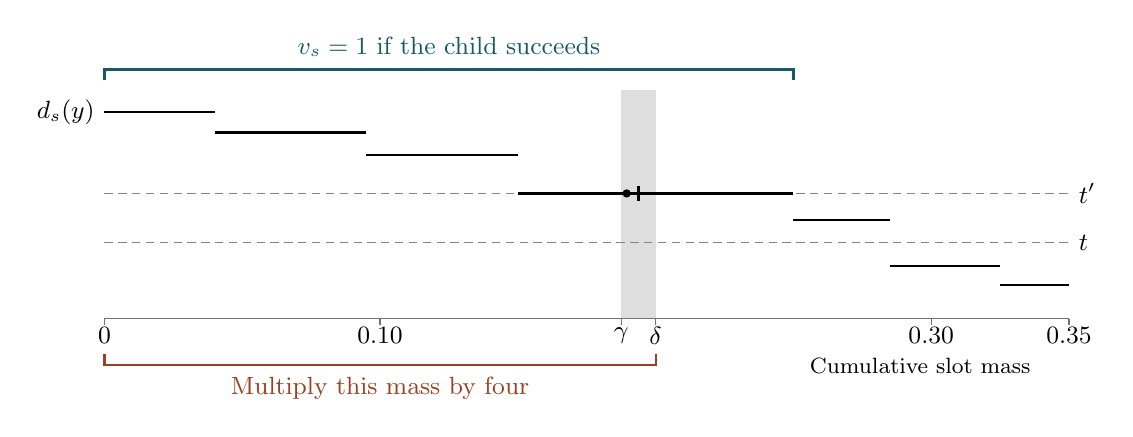
\begin{tikzpicture}[
  x=35cm,y=.86cm,font=\small,
  slot/.style={black,line width=.87pt},
  guide/.style={black!48,densely dashed,line width=.4pt},
  axis/.style={black!55,line width=.45pt},
  bracket/.style={line width=.8pt}]
 % Show the first .35 of the unit mass interval at its actual scale.
 \fill[black!13] (.1875,0) rectangle (.20,3.38);
 \draw[guide] (0,1.85) -- (.35,1.85) node[right,text=black] {\(t'\)};
 \draw[guide] (0,1.12) -- (.35,1.12) node[right,text=black] {\(t\)};
 \node[anchor=east] at (0,3.05) {\(d_s(y)\)};
 \foreach \a/\b/\h in {
   0/.04/3.05,.04/.095/2.75,.095/.15/2.42,
   .15/.19375/1.85,.19375/.25/1.85,.25/.285/1.46,
   .285/.325/.78,.325/.35/.50}
   \draw[slot] (\a,\h) -- (\b,\h);
 % A vertical tick separates the two slots with the same surplus.
 \draw[slot] (.19375,1.74) -- (.19375,1.96);
 \fill (.1895,1.85) circle[radius=1.5pt];

 \draw[axis] (0,0) -- (.35,0);
 \foreach \x/\lab in {0/0,.10/0.10,.1875/\gamma,.20/\delta,.30/0.30,.35/0.35}{
   \draw[axis] (\x,0) -- (\x,-.1);
   \node[below=2pt,inner sep=1pt] at (\x,0) {\(\lab\)};
 }
 \node[anchor=north,font=\footnotesize] at (.296,-.44) {Cumulative slot mass};
 \draw[bracket,lagoon] (0,3.52) -- (0,3.68) -- (.25,3.68) -- (.25,3.52);
 \node[above=1pt,text=lagoon] at (.125,3.68) {\(v_s=1\) if the child succeeds};
 \draw[bracket,ember] (0,-.52) -- (0,-.68) -- (.20,-.68) -- (.20,-.52);
 \node[below=1pt,text=ember] at (.10,-.68) {Multiply this mass by four};
\end{tikzpicture}
\caption{A heavy probe, with the first \(0.35\) of the slot mass shown.
Each horizontal segment represents a slot, ordered by surplus. The dot selects
a pivot in the shaded band \([\gamma,\delta)=[3/16,1/5)\).
Two adjacent slots have the pivot surplus \(t'\). Success at \(t'\) guarantees
correct feedback on mass \(0.25\), including both tied slots.
Reweighting multiplies the first \(0.20\) of the mass by four before normalization.}
\label{fig:band}
\end{figure}


\paragraph{Leaves.}
Take the root at level zero, all leaves at level \(D\),
the least positive odd number with
\[
               (5/4)^D>2N .
\]
At a leaf, return the coordinatewise median of the \(D\)
price vectors in the history.

\begin{lemma}\label{lem:leaf}
Each leaf succeeds: its returned prices achieve maximum surplus
at most its threshold, for any assignment as above.
\end{lemma}
\begin{proof}
Otherwise surplus at some slot \(s\) exceeds the leaf's threshold
at the median. This also happened at more than half of the
\(D\) proposals on the path.
Since thresholds never decrease, at each such proposal \(y\)
we had \(d_s(y)>t'\), with \(t'\)
the threshold assigned to the child. Thus the slot's weight was boosted by
a factor of at least \(4^{D/2}\) over the path before accounting for
normalizations. Starting from mass \(1/|S|\),
the slot has ended with at least
\[
       \frac1{2N}\frac{4^{D/2}}{(1+3\delta)^D}>1 ,
\]
a contradiction.
\end{proof}

Recursive amplification with reweighting also appears in the
contraction algorithm of Soleymani and Farina~\cite[\S6]{SF} and the
mean-payoff game algorithms of~\cite{OAIDe,OAIRa,OAITu}. In
\cite[\S\S3--5]{OAIDe}, near-extreme deviations of hidden vectors imply
shifted labeling requirements deeper in the recursion. That work
also discusses the relation to Parys's recursion~\cite{Parys}.

\subsection{Betting on a few slots}

If a majority of probes are light and their children succeed, the
parent succeeds because those children met the parent's own threshold.
A successful child in a heavy probe gives a different guarantee:
feedback is correct on the slots at or above the pivot surplus, a set
of mass at least \(\gamma\). Four independent draws from \(m\) hit
that set with probability at least \(1-(1-\gamma)^4>1/2\).
This probability is the reason four slots suffice.

The algorithm uses the same pool \(E\) in every probe. An expert
specifies the following data.

\begin{itemize}
 \item four slots in \(\Slots\) (an ordered tuple),
 guessing an integer demand in \([-R,R]\) on each;
 \item either threshold zero, or a level \(j\in\{0,\ldots,D-1\}\)
 and pivot slot in \(\Slots\), again guessing such a demand on that slot.
\end{itemize}
Include all such experts (repetitions of slots allowed, even with
different demands).
Zero-threshold experts always bid; those who specify \(j\)
only bid at levels deeper than \(j\)
(otherwise they have only the outside option, giving zero gain).

In bidding on its four slots, an expert shifts
its guessed demands by \emph{subtracting} its threshold estimate \(\tau\).
For an expert specifying \(j\),
\(\tau\) is the surplus
on its pivot slot at the proposal at level \(j\) in the price history,
using its guess for the pivot demand; \(\tau\) may even be negative.
For zero-threshold experts \(\tau=0\).
Thus bidding gives the four option utilities
\[
                b-\tau-y_s
\]
(one for each tuple position, with slot \(s\) and guess \(b\)).
As before, experts keep the outside option of utility zero,
and gains use the feedback \(v\) with worst tie breaking.

We analyze again with a consistent hypothesis and thresholds
assigned as above.
At each node consider a distribution \(\nu\)
of experts: sample the four slots independently from \(m\),
match this node's threshold description (including pivot
and level if used), and use true demands throughout.
Thus for these experts \(\tau=t\)
and sampled slot utilities are \(d_s(y)-t\).

\begin{lemma}\label{lem:gain}
Fix a consistent hypothesis and any threshold assignment as in
Section~\ref{sec:amplify}, and set \(\eta=1/16\).
In any probe where the child succeeds, for market gains
at the proposal \(y\) we have
\[
 \sum_e \nu_e \ln(1+\eta g_e)\ge
 \begin{cases}
   0 & \text{if light},\\
   \epsilon:=1/256 & \text{if heavy}.
 \end{cases}
\]
Here \(\nu\) is from the parent node.
\end{lemma}
\begin{proof}
In the light case with \(t'=t\),
for these experts every maximizing option gets
nonnegative feedback by~\eqref{eq:correct}
(including zero on the outside option).

In the heavy case with \(t'>t\),
if the tuple hits \(\{s:d_s(y)\ge t'\}\),
the gain is one: every maximizing option has surplus at least
\(t'\) and hence correct sign, with no tie from the outside option.
This happens for mass at least \(1-(1-\gamma)^4\) of~\(\nu\).
Since gains are always at least \(-1\),
mean gain is at least
\(1-2(1-\gamma)^4>1/8\).
The bound follows from \(\ln(1+\eta g)\ge\eta g-\eta^2\)
for these gains.
\end{proof}

Consider running these markets independently at every internal node,
with unit initial wealth and an odd number of probes greater than
\((2/\epsilon)\ln|E|\). Suppose all the children succeed. If half or
more of the probes are heavy, then Lemma~\ref{lem:gain} makes the
final log wealth, averaged under the fixed parent distribution
\(\nu\), greater than \(\ln|E|\). Yet no expert can exceed the
initial total wealth \(|E|\). A majority of the probes must be
light, so the median rule gives success. Lemma~\ref{lem:leaf} starts
this induction at the leaves.

The resulting tree has logarithmic depth and \(O(\log |E|)\) children
at each internal node. To obtain a polynomial bound on its size we
reduce the branching to a constant below the root. A child may then
miss its threshold. The following wealth update lets its parent still
make progress on that probe.

\subsection{Investing recursively}

Give the child a small share of each expert's wealth and retain the
rest for the parent's market. If the child misses its threshold, we
will show that some experts earn sufficiently large returns there
to cover what they might lose on the feedback it supplies. Use the
tree of Section~\ref{sec:amplify}, the expert pool \(E\), the rate
\(\eta=1/16\), and absolute constants

\begin{equation}\label{eq:probepars}
      c=2^{-14},\qquad r=2^{19}+1 .
\end{equation}
Give each internal node \(r\) probes except the root, which gets
\[
       r_0=r+3072\lceil\log(|E|+1)\rceil .
\]

Each node receives as input the price history and
a vector giving each expert positive wealth.
At the root, start with wealth one each.
Each node returns prices as well as a new wealth vector.
A leaf simply returns median prices from the history,
and returns the input wealth unchanged.

At an internal node, use the probes successively, starting with
the input wealth and keeping any changes across probes.
In each probe, split the current wealth \(w\) as shown in
Figure~\ref{fig:invest}:
\begin{enumerate}
 \item Use \((1-c)w\) in the market:
  take proposal prices \(y\) minimizing \(\Phi\) with that wealth.
  \item Call the child with \(y\) added to the history
  and with wealth \(c w\);
  let \(x\) and \(w'\) be the prices and wealth returned by the child.
  \item Query labels at~\(x\) and take feedback~\eqref{eq:feedback}.
  Replace \(w_e\) for each expert~\(e\) by
  \begin{equation}\label{eq:invest}
       (1-c)w_e(1+\eta g_e) + w'_e ,
  \end{equation}
  using the gains in this probe's market.
 \end{enumerate}
Return median prices from the children,
and the wealth vector after the last replacement.

Output the prices returned by the root.
We leave implementation of the markets (including deterministic
choices of minimizers) for later in this section.

\begin{figure}[htbp]
\centering
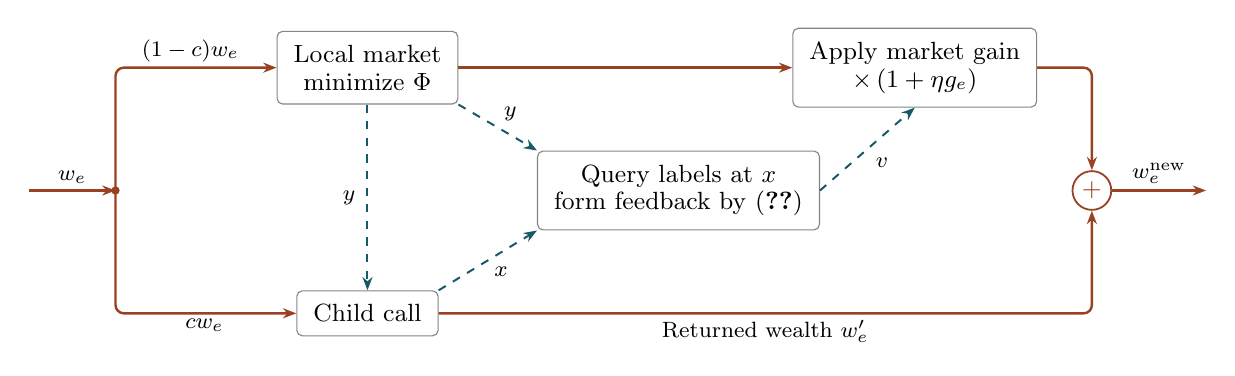
\begin{tikzpicture}[
  x=1cm,y=1cm,font=\small,
  box/.style={draw=black!48,fill=white,rounded corners=2pt,align=center,
              inner xsep=6pt,inner ysep=5pt},
  cash/.style={draw=ember,line width=.88pt,rounded corners=3pt,
               -{Stealth[length=4.8pt]}},
  data/.style={draw=lagoon,dashed,line width=.72pt,-{Stealth[length=4.8pt]}},
  note/.style={font=\footnotesize,inner sep=2pt}]
 \coordinate (split) at (1.1,0);
 \node[box] (market) at (4.3,1.56) {Local market\\[-1pt]minimize \(\Phi\)};
 \node[box] (child) at (4.3,-1.56) {Child call};
 \node[box] (feedback) at (8.25,0) {Query labels at \(x\)\\[-1pt]form feedback by \eqref{eq:feedback}};
 \node[box] (gain) at (11.25,1.56) {Apply market gain\\[-1pt]\(\times\,(1+\eta g_e)\)};
 \node[circle,draw=ember,text=ember,line width=.65pt,inner sep=1.6pt]
       (sum) at (13.5,0) {\(+\)};

 \draw[cash] (0,0) -- (split) node[midway,above,note] {\(w_e\)};
 \fill[ember] (split) circle[radius=1.5pt];
 \draw[cash] (split) -- (1.1,1.56) -- (market.west);
 \node[above,note] at (2.05,1.56) {\((1-c)w_e\)};
 \draw[cash] (split) -- (1.1,-1.56) -- (child.west);
 \node[below,note] at (2.23,-1.56) {\(c w_e\)};
 \draw[cash] (market.east) -- (gain.west);
 \draw[cash] (gain.east) -- (13.5,1.56) -- (sum.north);
 \draw[cash] (child.east) -- (13.5,-1.56)
             node[midway,below,note] {Returned wealth \(w'_e\)} -- (sum.south);
 \draw[cash] (sum.east) -- (14.95,0)
             node[midway,above,note] {\(w_e^{\rm new}\)};

 \draw[data] (market.south) -- (child.north)
             node[midway,left=2pt,note] {\(y\)};
 \draw[data] (market.south east) -- (feedback.north west)
             node[midway,above right=0pt,note] {\(y\)};
 \draw[data] (child.north east) -- (feedback.south west)
             node[midway,below right=0pt,note] {\(x\)};
 \draw[data] (feedback.east) -- (gain.south)
             node[midway,below right=1pt,note] {\(v\)};
\end{tikzpicture}
\caption{Wealth and prices in one probe. Solid arrows track the two shares of
expert \(e\)'s wealth. Dashed arrows show how the proposal \(y\) and the
child's price vector \(x\) determine the feedback \(v\) for the local market.
The sum \(w_e^{\rm new}=(1-c)w_e(1+\eta g_e)+w'_e\) funds the next probe
or, after the last probe, returns to the parent.}
\label{fig:invest}
\end{figure}


Every node returns total wealth at most its input total. At a leaf the
two totals agree. At an internal node~\eqref{eq:market} bounds the
wealth paid by the market by its initial share, while the same claim
for the child bounds its returned share. Recombining the two bounds
and iterating over probes proves the claim.

\subsection{Profits cover failures}

Fix a consistent hypothesis. We will prove that a failed node gives a
large return on its input wealth, averaged over experts whose demands
agree with that hypothesis. This assertion is local: those experts may
have had little wealth when they entered the node. At the root, however,
every expert starts with wealth one and the total is at most \(|E|\).
There a sufficiently large return is impossible.

At each node let
\[
  \mu_e = \frac{\text{returned wealth for }e}
                     {\text{input wealth for }e},
       \qquad L_e = \ln(1+(c/2)\mu_e)
\]
for each expert.
Use \(L_e\) to count the bonus from returns here,
as a contribution to log wealth one level up.
Indeed, if in a probe the child has such values
\(\mu'_e,L'_e\), the wealth multiplier from~\eqref{eq:invest} is
\[
    (1-c)(1+\eta g_e)+c\mu'_e \ \ge\
    (1-c)(1+\eta g_e)\cdot (1+(c/2)\mu'_e)
\]
as \((1-c)(1+\eta g_e)<2\).
Consequently for any internal node,
\begin{equation}\label{eq:bonus}
 L_e\ \ge\ -\ln(2/c)+
     \sum_{\text{probes}}
     \big(\ln(1-c) + \ln(1+\eta g_e)+L'_e\big),
\end{equation}
by taking logs and summing to bound \(\ln\mu_e\).
For each term, the primed value is from that probe's child.
Each \(L'_e\) is nonnegative, even if the child's investment lost
wealth. Thus \(-\ln(1-c)\) bounds the loss per probe from sending
wealth to the child, while a large child return gives an additional
positive term.

To use a child's return in~\eqref{eq:bonus}, we must average its
bonuses with the parent's expert weights. The distribution \(\nu\)
from Lemma~\ref{lem:gain} samples four slots and specifies the
\emph{current} threshold. A heavy probe gives the child a new pivot
description, so its \(\nu'\) can be disjoint from the parent's \(\nu\).
We reserve weight at the parent for experts with each possible future
pivot level, including the one at which this probe takes place.

\paragraph{Comparing expert weights across one probe.}
For a fixed assignment of thresholds, give each node at level \(l\)
the following nonnegative weights \(\pi\) on the experts.

\begin{itemize}
 \item Include \(\nu\):
 the distribution with tuple slots i.i.d.\ drawn from~\(m\),
 matching this threshold description and using true demands.
 \item For each possible \emph{future} pivot level
 \(j\in\{l,\ldots,D-1\}\),
 include mass \(2^{l-j}\), distributed by picking four slots
 and the pivot slot at that level all independently from \(m\),
 with true demands. These experts have zero gains in the markets
 at this node, because they bid only deeper in the tree.
\end{itemize}
Thus~\(\pi\) is nonnegative of total mass at most three.

\begin{lemma}\label{lem:transfer-p}
For a complete run and a consistent hypothesis, there is an
assignment (choosing all thresholds and pivots as allowed in
Section~\ref{sec:amplify}) such that in every probe
\[
        \sum_e \pi'_e L'_e \ \le\ C \sum_e \pi_e L'_e ,
         \qquad C=80(5/2)^4=3125
\]
where \(\pi,\pi'\) refer to the parent and child respectively,
and \(L'\) is the vector of bonuses at the child.
\end{lemma}
\begin{proof}
Proceed down the tree. With \(m,t,\pi\) already determined for a
node, consider choosing the pivot in any heavy probe here at random:
take a uniform point in the band
\([\gamma,\delta)\) to determine the pivot slot.
This spreads out the choice: for any slot, the probability
is at most \(1/(\delta-\gamma)=80\) times that under \(m\).

We claim \(\EE\pi'\le C\pi\) componentwise, including a light probe
with its prescribed threshold. The child distribution \(m'\) is already
fixed before choosing the pivot. Since \(m'\le4m/(1+3\delta)=(5/2)m\),
sampling the four tuple slots costs a factor of at most \((5/2)^4\).

\begin{itemize}
 \item For the child's mass with its current threshold description:
if light, compare with the parent's such mass,
since the description does not change.
If heavy, compare instead with the parent's future mass for
\(j=l\), using the extra factor of 80 for the chosen pivot.
 \item For the child's future mass at any pivot level \(j\ge l+1\),
compare with the parent's future mass for that level.
Beyond the factor for the four slots there is a factor two
for total mass for that level, and at most \(5/2\)
for the pivot slot probabilities.
\end{itemize}
The parent's current description and its reserve for each future
level are distinct expert classes. The componentwise comparisons can
therefore be combined with the single factor \(C\).

The entire run was fixed before choosing pivots, so the child bonuses
\(L'_e\) are fixed nonnegative numbers. Multiplying the componentwise
expectation bound by \(L'_e\) and summing shows that at least one allowed
pivot satisfies the claimed inequality. Fix such a choice in every
heavy probe at this level and continue to the next level.

\end{proof}

\begin{lemma}\label{lem:charge}
For a consistent hypothesis, assign thresholds as in
Section~\ref{sec:amplify}, with the pivots chosen as in
Lemma~\ref{lem:transfer-p}.
If an internal node fails and has \(T\) probes, then
\begin{equation}\label{eq:charge}
           \sum_e \pi_e L_e\ \ge\ \sigma T,\qquad
           \sigma=\epsilon/4=1/1024 .
\end{equation}
\end{lemma}
\begin{proof}
Proceed from the bottom of the tree.
Fix such a node.
We bound the contribution
\(
   \sum_e\pi_e (\ln(1+\eta g_e)+L'_e)
\)
in~\eqref{eq:bonus} per probe.
\begin{itemize}
 \item The child succeeds:
 the contribution from log market gains
 \(\ln(1+\eta g_e)\)
 is nonnegative, and at least \(\epsilon\)
 if heavy, by Lemma~\ref{lem:gain}
 (the experts added for future pivots have gain zero).
 Child bonuses only help.
 \item The child fails:
 then the child must be internal by Lemma~\ref{lem:leaf}.
 Therefore
 \[
    \sigma r\le
         \sum_e \pi'_e L'_e
        \le C\sum_e \pi_e L'_e
 \]
 by induction and the choice of pivots. Thus this probe contributes at least
 \[
       \ln(1-\eta)+\frac{\sigma r}{C}
       \ge -2\eta+\frac{\sigma r}{C} \ge\epsilon ,
 \]
 paying for possibly bad market outcomes
 (again future-pivot experts have zero gain).
\end{itemize}
By the median rule, failure implies that for a majority
of probes either the probe was heavy or the child failed.
So altogether
\[
   \sum_e \pi_e L_e\ \ge\
      T\epsilon/2
          -3T(2c)-3\ln(2/c)\ \ge\ \sigma T
\]
by~\eqref{eq:bonus}, \(\ln(1-c)\ge-2c\),
and the choices~\eqref{eq:probepars}
(\(6c<\epsilon/8,\ 3\ln(2/c)<r\epsilon/8,\ T\ge r\)).
\end{proof}

At the root, \(\mu_e\le|E|\)
since the total wealth cannot increase,
so \(L_e\le\log(|E|+1)\)
(recall \(\log\) denotes base two).
As \(\sigma r_0>3\log(|E|+1)\),
there cannot be a failure: apply Lemma~\ref{lem:charge}
with assignments as in Lemma~\ref{lem:transfer-p}.
As this holds for any hypothesis consistent with all answers,
the returned prices meet all demands as required.

\subsection{Running the markets}\label{sec:implement-pr}

The number of probes is \(O(r_0r^{D-1})\). The expert choices give
\(|E|\) polynomial in \(N,R\), so \(r_0=O(\log(NR+1))\).
Since \(D\) is the least positive odd integer with \((5/4)^D>2N\)
and \(\log_{5/4}r<60\), the tree uses \(O(N^{60}\log(NR+1))\)
probes. The wealths also have polynomial bit length. Each probe adds
only constantly many binary places to a common dyadic denominator,
and all wealths are bounded by the root's initial total \(|E|\).

The remaining cost is choosing the proposal at each probe. We first
bound its bit length and then describe how to optimize over the
implicit expert pool in time polynomial in \(N,\log(R+1)\).

\paragraph{Prices at vertices.}
At each probe use an optimum vertex of the epigraph of~\(\Phi\).
Such vertices exist. Indeed, \(\Phi\) even tends to infinity
as \(\|y\|_\infty\) grows:
there are zero-threshold experts whose tuples
repeat a single slot with guess zero, one for each slot,
with strictly positive wealth.
Thus the optimal face is nonempty and bounded.

We claim this keeps all prices half-integral, with polynomial bit
length, through the tree. To see this, a vertex price vector
is determined by ties in each expert's option utilities, i.e.,
by equations equating utilities of options of the same expert
(including ties with the outside option).
Indeed, otherwise there is a line through the price vector
preserving all those ties; each \(U_e\), hence also \(\Phi\),
is affine near the point on this line, contradicting extremality.
Equations from equating two slot utilities have form
\[
      y_i = \pm y_j + B,\qquad B\in\ZZ,\quad |B|\le2R ,
\]
as the \(\tau\) is common. Within any connected component of these edges
on the \(N\) coordinates, express all its prices in terms of
one of them via a spanning tree.
If these equations in the component already determine the prices there,
some remaining edge (possibly a loop) determines twice
that one price as an integer of magnitude \(O(NR)\).
If not, a tie with the outside option must pin some price in the component,
to an integer or to a signed history price plus an integer
(in either case with the integer bounded by \(2R\)
in absolute value).
By induction down the tree we keep half-integrality
and prices of magnitude \(O(DNR)\).

\paragraph{Cells of experts.}
Group experts by all their data except their
demand guesses. Thus the number of groups is polynomial, and
each group corresponds to the integer points of a box
(one dimension per guess, at most five).
Observe that for given prices (proposal and history),
all comparisons among an expert's option utilities are
comparisons of single guesses or differences of two guesses
against constants. Thus we can subdivide the groups
by these comparisons, creating cells of experts with a common
set of maximizing options (by position on their lists).

More precisely, within each group partition
the range \([-R,R]\) for each guess into intervals of integers,
and similarly partition \([-2R,2R]\) for each pairwise difference.
Choosing one interval from each partition gives a cell of experts,
requiring all of the bounds simultaneously
(the cell may be empty). Start with each range as one interval.
Every time we choose proposal prices,
refine according to all of the option comparisons with these
prices, keeping ties separate.
Each partition now gets only a constant number of new cuts per probe,
and each group has only
a constant number of partitions.
Thus the number of cells remains polynomial.

The outcomes (including ties) of all option comparisons at
proposals so far are now common within cells.
So gains in response to feedback are also common:
we can identify all maximizing options at the proposal.
Wealths too are common, since splits, updates and recombination
preserve this.
Keep these per-expert data for each cell,
copying them upon refinement to the subcells.
This includes wealth data for any ongoing probes, which
we need to recombine wealths.
Compare Feodorov and Haslebacher's use of arrangements and volumes
for fixed points~\cite{FH};
here each expert has only a constant-dimensional guess,
regardless of \(N\).

To use these cells in choosing prices, we compute two kinds of sums:
the number of experts in a given cell, and the sum there of any
given guess coordinate.
In fact we can sum polynomials by eliminating variables one by one.
The range for a variable to eliminate runs from a maximum
of lower bounds to a minimum of upper bounds,
each bound an integer constant or a remaining variable plus
an integer constant.
So, on the remaining variables, we can subdivide according to which
bounds achieve these two extrema (choose first in case of ties),
and require lower at most upper.
All these conditions have the same form (interval constraints on
variables and differences). On each piece, summing over this range
again gives a polynomial by the formulas for sums of powers
(discrete antiderivatives, valid also with negative endpoints).
Starting with constant and linear polynomials for our computations,
the degree goes up by at most one per step, and bounds and coefficients
undergo only constantly many arithmetic operations:
both branching and depth are bounded by constants.
This gives the sums in polynomial bit complexity.

\paragraph{Computing the market minimizer.}
The label oracle is queried at prices returned by the children.
To choose the parent proposal, we construct a separate oracle from the
finite market data. It separates points from the epigraph of \(\Phi\),
which is defined by one inequality for every selection of one option
per expert: the height must dominate their weighted sum of utilities.
These inequalities have polynomial bit length because the history
prices are short, the weights share a short denominator, and \(\log|E|\)
is polynomial in the input size.

At rational test prices, compute an affine sum as above attaining
\(\Phi\).
To do so, temporarily refine on the option comparisons at
these prices. Choose a common maximizing option for the experts
in each cell and compute the coefficients from their weighted utilities
using counts and sums of guesses.
This gives separation: compare the proposed height to \(\Phi\)
and use the computed inequality if violated (the normal can be
scaled to sup norm one).
The bit time is polynomial, counting also the bits of the test point
as input.

Apply the classical bit-polynomial ellipsoid algorithm for
well-described polyhedra~\cite[Theorem~(6.4.9)]{GLS} to this separator.
All data passed to it have the bit bounds just proved. This is the
LP subroutine used to implement~\eqref{eq:market}.

Add the optimal height constraint
(still polynomial bits), and take
the lexicographically first optimal point,
a vertex (cf.~\cite[Lemma~(6.5.1)]{GLS}),
minimizing each coordinate successively.
This works in polynomial time as well:
the optimal face is bounded,
and each additional constraint value fixing a price coordinate
is a coordinate of the final vertex,
hence still short.

This gives the required deterministic implementation;
medians and labels too use polynomially many bits,
and the bounds hold regardless of labels.
This proves Theorem~\ref{thm:prices} and so completes
the proof of Theorem~\ref{thm:lp}.

\section{Quadratic programming and complementarity}\label{sec:quadratic}

At a minimum of a convex quadratic over a polyhedron, each inequality
has either zero slack or zero multiplier. If we knew which entry to set
to zero in every pair, we could recover the point and its multipliers
by solving linear equations and inequalities. We find those zeros by
applying the pricing method of Section~\ref{sec:lp} to the more general
monotone linear complementarity problem~\cite{CD,CPS}.

Given \(M\in\RR^{N\times N}\) and \(q\in\RR^N\), the linear
complementarity problem asks for \(z,w\in\RR^N\) satisfying
\begin{equation}\label{eq:lcp}
 z\ge0,\qquad w=Mz+q\ge0,\qquad z^\top w=0 .
\end{equation}
Here \(M\) is \emph{monotone}, meaning \(M+M^\top\succeq0\).
Nonnegativity makes the last equality equivalent to \(z_iw_i=0\)
for every \(i\).

\begin{theorem}[Monotone linear complementarity]\label{thm:lcp}
There is a deterministic strongly polynomial algorithm
that, for any monotone linear complementarity
problem~\eqref{eq:lcp},
returns a solution or an infeasibility certificate \(u\ge0\)
satisfying \(M^\top u\le0\) and \(q^\top u<0\).
\end{theorem}

For convex quadratic programming the earlier bit-polynomial algorithm
is due to Kozlov, Tarasov and Khachiyan~\cite{KTK}. Interior-point
methods for monotone complementarity include those of Kojima, Mizuno
and Yoshise~\cite{KMY}. Granot and Skorin-Kapov obtained Tardos-type
bounds with matrix dependence for strictly convex quadratics~\cite{GSK},
and Cui, Li and Miao obtained such bounds for separable
quadratics~\cite{CLM}. V\'egh's strongly polynomial algorithms for
network flows with convex costs include separable quadratic costs~\cite{VQ}.

Monotonicity enters at two distinct steps. It ensures that feasibility
of the linear constraints in~\eqref{eq:lcp} suffices for existence of a
complementary solution. To \emph{find} one, we also use it to construct
a convex set that approximates every scaled, normalized solution
and has small complementarity gap throughout. The midpoint argument of
Lemma~\ref{lem:mid} then makes the coordinate labels unambiguous.

\subsection{Linear feasibility and existence of a solution}

By Cottle's theorem~\cite{Cottle}, a monotone LCP has a solution
whenever its linear constraints are feasible. For the proof, we first
record the attainment argument for convex quadratics, which will also
give the unboundedness certificate in Corollary~\ref{cor:qp}.

Consider \(\tfrac12 x^\top Gx+c^\top x\) on a nonempty polyhedron
\(\{x:Ax\le b\}\), where \(G\) is symmetric positive semidefinite.
The Frank--Wolfe attainment theorem~\cite{FW} in this setting follows
from the following alternative. There may be a direction

\begin{equation}\label{eq:baddir}
 d:\quad Ad\le0,\qquad Gd=0,\qquad c^\top d<0,
\end{equation}
giving rays of descent to \(-\infty\). Otherwise
\(c=Gv-A^\top\mu\) for some \(v,\mu\) with \(\mu\ge0\), by Farkas.
Writing \(G=T^\top T\), the objective is then
\[
 \tfrac12\|T(x+v)\|_2^2-\mu^\top Ax+\mathrm{const}.
\]
The pairs \((T(x+v),\mu^\top Ax)\) attainable with \(Ax\le b\)
form a polyhedron, with second component bounded above.
So in this image space the objective has compact sublevel sets
on the polyhedron. There is an optimum.


Now minimize
\(z^\top w\), \(w=Mz+q\), subject to \(z,w\ge0\).
If feasible there is an optimum by attainment, since the objective
is a convex quadratic and bounded below by zero.
Any such optimum solves the LCP. Indeed, in the variable \(z\)
it also minimizes the linearization there, so by LP duality
there are multipliers \(u,v\ge0\) with
\[
 w+M^\top z=v+M^\top u,\qquad w^\top u=z^\top v=0.
\]
Dotting the stationarity equation (with all terms on the left)
with \(z-u\) gives
\[
 z^\top w+u^\top v+(z-u)^\top M(z-u)=0.
\]
All three terms are nonnegative, proving the claim.

\subsection{Labeling for complementarity}

First use Theorem~\ref{thm:lp} to test the linear constraints
\(-z\le0,\ -Mz\le q\). In the infeasible case, the Farkas
multipliers on \(-Mz\le q\) form the desired certificate \(u\).
In the feasible case with \(q=0\), take \(z=w=0\). For \(q\ne0\)
collect the scaled affine spaces in the single linear subspace
\[
 W=\{(z,Mz+\alpha q):z\in\RR^N,\ \alpha\in\RR\}.
\]
View these vectors \(y=(z,w)\) as rows when used with bases
and scalings. Use positive slots for \(z\), negative for \(w\),
so \(Q(y)=z^\top w\). Use as row basis \(B_0\)
a basis of the directions with \(\alpha=0\), say from unit vectors
in the \(z\)-space, followed by \((0,q)\).


Choose a solution \(y\), with \(\alpha=1\), of minimal support.
It is a circuit of \(W\). Indeed, if the subspace supported on
\(\supp y\) had dimension at least two, the linear functional
\(\alpha\) would vanish on a nonzero vector there. Move from \(y\)
in one of the two directions along this vector until a positive
entry first reaches zero. The resulting vector still has
\(\alpha=1\), all its entries are nonnegative, and it retains at
least one zero in each pair. It would therefore be a solution
of smaller support.

As before, apply calibration (Theorem~\ref{thm:cal})
and the extremal price theorem (Theorem~\ref{thm:prices}),
restarting price search on a calibration restart.
Use the same parameters~\eqref{eq:labelpars}.
At a queried price vector let \(B_*=LB_0D\)
be the true basis corresponding to the answer \(B\)
as in Theorem~\ref{thm:cal}.
Our task is to give label \(h\) at \(i\)
if slot \((i,h)\) maximizes surplus for such a solution circuit
(with its calibrated demands).
After scaling the circuit by \(D\) and normalizing, the entry
at such a slot is at least \(1/3\).
As in LP we will test for large entries using only \(B\).
To avoid conflicting labels, we again want
a convex set of candidates on which \(Q\) is uniformly small,
to use the midpoint argument (Lemma~\ref{lem:mid}).
We develop the constraints first with the true basis.

\paragraph{A convex constraint for a scaled solution.}
With the reciprocal scaling \(D\), the complementarity gap
\(Q(y)=z^\top w\) is unchanged. On the subspace with \(\alpha=0\),
the gap is \(z^\top Mz\ge0\). The first \(N\) rows of \(B_*=LB_0D\)
span this subspace after scaling because \(L\) is lower triangular.
The last diagonal entry of \(L\) is positive, so a vector with
\(\alpha>0\) has a positive coefficient on the last row.

Write the row coefficients as \(\xi=(v^\top,\lambda)\) with
\(v\in\RR^N\). Gathering the terms that contain \(\lambda\) gives
\[
 Q(\xi B_*)=v^\top A_*v-\lambda g_*(\xi),
\]
where \(A_*\) is symmetric positive semidefinite and \(g_*\) is
linear. In the scaled, normalized representation of a solution,
\(\lambda>0\) and \(Q(\xi B_*)=0\). Hence
\(g_*(\xi)=v^\top A_*v/\lambda\ge0\). Every such solution belongs to
the convex set
\[
 \lambda\ge0,\qquad g_*(\xi)\ge0,\qquad
 v^\top A_*v\le \lambda g_*(\xi).
\]
Indeed, \(\sqrt{v^\top A_*v}\) is a seminorm and the geometric mean of
the two nonnegative quantities on the right is concave. This is the
rotated second-order cone constraint in the coordinates of \(B_*\).

\paragraph{A label test on the rational basis.}
With \(B\), use again the decomposition
\(Q(\xi B)=v^\top A v-\lambda g(\xi)\),
taking \(A\) symmetric as before. Recall \(H=2^{100N^2}\),
\(\epsilon=H^{-10}\), and set
\(
 \widetilde A=A+H^{-50}I.
\)
Use candidates \(y=\xi B\)
as in~\eqref{eq:box}
(again with \(\|\xi\|_\infty\le H\),
\(-\epsilon\le y_s\le 2\) for each entry),
with the \emph{additional} constraints
\begin{equation}\label{eq:rot}
 \lambda\ge0,\qquad
 g(\xi)+\epsilon\ge0,\qquad
 v^\top \widetilde A v\le(\lambda+\epsilon)(g(\xi)+\epsilon).
\end{equation}
These height shifts let us work with only absolute accuracy on the
basis entries,
even when a solution has \(\lambda\) tiny or \(g_*(\xi)=0\).


Indeed, \(B\) is within \(H^{-100}\) of \(B_*\),
which is bounded by \(2\) entrywise. Hence \(A,g\) are within
\(20NH^{-100}\) of \(A_*,g_*\) coefficientwise, by taking dot
products. Thus \(\widetilde A\) is positive semidefinite,
so the constraints are convex together as before.
Also for \(\|\xi\|_\infty\le H\),
\[
 |g(\xi)|\le H^2,\qquad
 |g(\xi)-g_*(\xi)|\le H^{-90},
 \qquad |v^\top(\widetilde A-A_*)v|\le H^{-45}.
\]
All candidates satisfy
\[
 Q(y)\le \epsilon(\lambda+g(\xi)+\epsilon)\le H^{-1}.
\]
And for any solution \(y_0\), write
\(y_0D/\|y_0D\|_\infty=\xi B_*\), with
\(\|\xi\|_\infty\le H\).
To see that \(y=\xi B\) is a candidate, observe that it approximates \(\xi B_*\) within \(\epsilon^2\)
entrywise, and~\eqref{eq:rot} holds since in particular
\[
 (\lambda+\epsilon)(g(\xi)+\epsilon)
 \ \ge\ \lambda g_*(\xi)+\epsilon^2/2
 \ \ge\ v^\top \widetilde A v.
\]


Assign \(+\) at \(i\) if the candidate set contains a point with
\(y_{i+}\ge1/4\), and assign \(-\) otherwise. Only short rational
data enter this test. To carry it out using the bit-polynomial convex
QP algorithm~\cite{KTK}, divide by the positive quantity
\(\lambda+\epsilon\). Introduce
\(s=1/(\lambda+\epsilon)\), \(\bar\xi=s\xi\) and \(\bar y=sy\).
Multiply every linear constraint, including the label threshold, by
\(s\), and impose
\[
 s\ge\frac{1}{H+\epsilon},\qquad
 \bar\lambda+\epsilon s=1,\qquad
 \bar v^\top\widetilde A\bar v\le g(\bar\xi)+\epsilon s,
 \qquad \bar\xi=(\bar v^\top,\bar\lambda).
\]
The last inequality is~\eqref{eq:rot} multiplied by \(s^2\).
Conversely, dividing the barred variables by \(s>0\) recovers the
original constraints. This perspective transformation~\cite[\S2.3.3]{Boyd}
leaves one convex quadratic inequality on a bounded polyhedron.
Indeed, \(\bar\lambda\ge0\) gives \(s\le1/\epsilon\), and the scaled
box constraints bound \(\bar\xi,\bar y\). Test linear feasibility
first. On a nonempty polyhedron, minimize the left side minus the right
side of the quadratic inequality and accept exactly when its minimum
is nonpositive.

\begin{proof}[Conclusion of the proof of Theorem~\ref{thm:lcp}]
As in LP, consider the final uninterrupted price search, with demands given by
calibration. A solution circuit, scaled and normalized at a query,
has entry at least \(1/3\) at each slot of maximal surplus on
its support. A candidate therefore reaches \(1/4\) at this slot.
No candidate can reach the same threshold at the opposite slot by convexity and
Lemma~\ref{lem:mid}. As a result the labels are consistent
with the solution circuit's demands.


Write \(x\) for the prices returned by the extremal price algorithm.
In each pair allow only one slot to be positive, namely at the
sign of \(x_i\) (arbitrary choice when zero).
Return to the original system~\eqref{eq:lcp}
and impose the indicated zeros.
Each demand on the solution circuit's support is positive and
met, so these zeros retain the solution circuit. Theorem~\ref{thm:lp}
recovers a solution of the resulting linear system.

The number and sizes of the label tests obey the same bounds as in
Section~\ref{sec:lp}. Their convex QP data have short binary
encodings. The two LP calls on the original data check initial
feasibility and recover the solution. All steps are deterministic.
\end{proof}

A single solution \((z_*,w_*)\) also gives a linear description of
the entire solution set~\cite{Man}. On the region \(z,w\ge0\),
\(w=Mz+q\), the identity
\[
 z^\top w=z^\top w_*+z_*^\top w+(z-z_*)^\top M(z-z_*)
\]
splits the gap into three nonnegative terms. Their sum is zero
precisely when
\[
 z^\top w_*+z_*^\top w=0,\qquad (M+M^\top)(z-z_*)=0 .
\]
The second equivalence uses positive semidefiniteness of \(M+M^\top\).
Consequently the solution set is a polyhedron. To find a solution of
maximum support, test which entries can be positive by linear
feasibility. Averaging the witnesses gives a solution positive on
all those entries at once.

\subsection{Quadratic optimization and conic feasibility}

The first-order optimality conditions for a convex quadratic are
an affine variational inequality~\cite{KT,KuhHist}. Their classical
complementarity formulation~\cite{CD,CPS} yields the following
algorithm.

\begin{corollary}[Convex quadratic programming and affine variational inequalities]\label{cor:qp}
Both problems below are solvable in deterministic strongly
polynomial time for arbitrary real data.
\begin{enumerate}
 \item \emph{Affine variational inequalities.} Given a polyhedron \(P=\{x\in\RR^n:Ax\le b\}\)
 and monotone \(G\in\RR^{n\times n}\), \(c\in\RR^n\),
 find \(x\in P\) such that
 \((Gx+c)^\top(x'-x)\ge0\) for all \(x'\in P\), or report
 that none exists.
 \item \emph{Convex quadratic programming.} For such \(P\) and symmetric \(G\succeq0\), minimize
 \(\tfrac12 x^\top Gx+c^\top x\) over \(P\), returning an
 optimum and multipliers, or certifying infeasibility or
 unboundedness.
\end{enumerate}
\end{corollary}


\begin{proof}
By LP duality the variational inequality at \(x\in P\) holds
if and only if there are multipliers satisfying
\[
 Gx+c+A^\top\mu=0,\qquad
 \mu\ge0,\qquad
 \mu^\top(b-Ax)=0.
\]
Write \(x=Ru\) for \(R=[I\ {-I}]\), with \(u\ge0\).
The requirements on \(u,\mu\) are exactly~\eqref{eq:lcp}
for
\[
 z=\binom{u}{\mu},\qquad
 M=\begin{pmatrix}
  R^\top GR & R^\top A^\top\\ -A R & 0
 \end{pmatrix},\qquad
 q=\binom{R^\top c}{b}.
\]
Indeed, applying \(R^\top\) includes each entry of
\(Gx+c+A^\top\mu\) and its opposite in the first block
of \(w\), forcing zero. Monotonicity is
immediate, so apply Theorem~\ref{thm:lcp}.

For the quadratic objective, first test feasibility of \(P\) by
Theorem~\ref{thm:lp}. If \(P\) is empty this gives a Farkas
certificate. Otherwise retain a feasible point \(x_0\) and test the
linear conditions~\eqref{eq:baddir} on \(d\). Any such \(d\) gives
the ray \(x_0+td\), \(t\ge0\), along which the objective decreases
to \(-\infty\). If no such direction exists, the attainment argument
gives a minimum. Convexity makes the variational inequality necessary
and sufficient for optimality, so the complementarity solution yields
an optimizer and its multipliers. These reductions use a constant
number of layers of scalar computations and calls as in
Section~\ref{sec:arithmetic}.
\end{proof}

The LCP and convex QP algorithms and their certificates transfer to
ordered fields by the argument in Section~\ref{sec:lp}. Diagonalizing
the symmetric form by congruence shows that its positive
semidefiniteness persists in a real closure.

\paragraph{Projection.}
For any \(v\) and any nonempty polyhedron \(P\), minimizing
\(\|x-v\|_2^2\) over \(P\) gives its Euclidean projection.
If a polytope is given by vertices, barycentric variables express
membership by linear constraints. This includes the minimum-norm
point of a vertex-given simplex.
See Hong and Verma~\cite{HV} for earlier connections of
strong polynomiality questions for convex QPs and projection, and
De Loera, Haddock and Rademacher~\cite{DLHR}
for an LP reduction \emph{to} the minimum-norm problem in an
integer-input model, as well as exponential behavior of Wolfe's
combinatorial algorithm \cite{W76}.
Fujishige, Kitahara and V\'egh~\cite{FKV} give bounds using circuit
imbalance for update-and-stabilize methods for box-constrained least
squares.

\paragraph{A conic consequence.}
Another short application, using perspective again,
is to a special case of second-order cone programming
(see~\cite{Lobo,Boyd} for background and applications).

\begin{corollary}[Lorentz constraints with proportional quadratic parts]\label{cor:lor}
One can deterministically decide, in strongly polynomial time,
real feasibility of linear weak inequalities together with a single
Lorentz constraint
\begin{equation}\label{eq:lor}
 \|F(x)\|_2\le h(x)
\end{equation}
for real affine maps \(F,h\) with vector and scalar output, respectively,
and return a point in case of feasibility.

More generally we can decide feasibility, within the same bound,
for arbitrarily many Lorentz constraints if the Hessians
\(\nabla^2(\|F(x)\|^2_2-h(x)^2)\)
(one for each constraint)
span at most one dimension
\textup{(}e.g., ball constraints of the form
\(\|x-c\|_2\le r\) for given \(c,r\)\textup{)}.
We can return an exact feasible point here using an output
representation \(a+b\sqrt d\),
giving scalar \(d\ge0\) and vectors \(a,b\)
in the field generated by the input.
\end{corollary}


\begin{proof}
In the single-constraint case,
test first for feasibility with \(h(x)=0\), by LP
(since we then just require \(F(x)=0\) for~\eqref{eq:lor}).
For \(h(x)>0\) use variables \(s=1/h(x),y=sx\),
writing the conditions as \(s>0\)
together with
\[
 Ay\le sb,\qquad H(y,s)=1,\qquad f(y,s):=\|T(y,s)\|_2^2\le1,
\]
with \(Ax\le b\) the given linear constraints and \(H,T\)
the linear forms or maps obtained by homogenizing
\(h,F\) using \(s\).
Find a point satisfying all but possibly the norm constraint
(or conclude infeasibility) by LP.
If this point does not already give a solution,
minimize \(f\) over the linear conditions with \(s>0\)
relaxed to \(s\ge0\),
by Corollary~\ref{cor:qp}.
A minimum greater than one proves infeasibility. If the minimum
is less than one, interpolate between its value and the value at the
point from LP, choosing a positive weight on the latter so the
interpolated value is one. The corresponding convex combination has
\(s>0\) and \(f\le1\) by convexity. If the minimum is one, we need
a minimizer with \(s>0\). Strict convexity of the squared norm in
the \(T\)-image makes that image the same at every minimizer.
Fix it to the value already found and test for \(s>0\) by LP.


Now for several constraints of the indicated type,
require the right-hand sides nonnegative and square the constraints.
Besides linear constraints the result has the form
\[
 \ell_j(x)\le q(x),\qquad q(x)\le r_k(x)\qquad(\text{respective indices }j,k)
\]
for affine \(\ell_j,r_k\) and one quadratic form \(q\),
after rescaling inequalities (all quadratic parts
are multiples of one).
Impose also all \(\ell_j(x)\le r_k(x)\).

On this linear region, test separately for feasibility with the
lower bounds, and for feasibility with the upper bounds.
For the lower bounds, try each \(j\) as a maximizing index. Impose
\(\ell_j\ge\ell_{j'}\) for all \(j'\) and enforce \(\ell_j\le q\)
using its original Lorentz constraint. The upper bounds are treated
in the same way by enumerating a minimizing index. If either list
is empty, its separate feasibility test consists of linear
constraints alone.
If there are both kinds, with feasibility for each separately,
consider the segment between the two witnesses. At each point, the lower
bounds all hold or the upper bounds all hold (since \(\ell_j\le r_k\)).
These are closed conditions, so somewhere on the segment both hold.
We can find such a point by testing endpoints and enumerating roots
of nonconstant quadratic or linear constraint polynomials on the
segment (an endpoint of the closed feasible portion suffices).
Testing at such a root takes ordinary scalar operations and comparisons
by isolating a radical and squaring (checking signs first).
Only constantly many layers of subroutine calls
or polynomial-size arithmetic formulas are needed,
so we get strong polynomiality as claimed.
\end{proof}

A radical in the generalization can be necessary for a witness.
For example, \(\|(2x,1)\|_2\le3\) and
\(\|(1,1)\|_2\le x\) together force \(x=\sqrt2\).

\section{Contractions in max norm}\label{sec:contractions}

At a point \(x\) far from a fixed point \(v\), a contraction in max
norm must move each coordinate of greatest error toward \(v\).
The signs of these movements give exactly the kind of partial
information used by Theorem~\ref{thm:prices}. We use them to locate
\(v\) with a running time polynomial in the number of bits of accuracy.

Let \(C=[-1,1]^n\), \(n\ge1\). A self-map \(f:C\to C\) with
\[
 \|f(x)-f(y)\|_\infty\le (1-\gamma)\|x-y\|_\infty,\qquad
 0<\gamma\le1,
\]
has a unique fixed point \(v\)~\cite{Ban}. Direct iteration may
require order \(1/\gamma\) evaluations to halve the error.
We assume an oracle that accepts a dyadic point \(x\in C\) and a
precision \(m\). It returns a dyadic point of \(C\) with \(m\) bits
after the binary point and sup norm error at most \(2^{-m}\) from
\(f(x)\). Dimensions and accuracy parameters are given in unary.

\begin{theorem}[Approximation in max norm]\label{thm:contraction}
For \(\gamma=2^{-b}\)
we can, given this access to the contraction \(f\)
and nonnegative integers \(b,k\), return
a dyadic \(x\in C\) with \(\|x-v\|_\infty\le 2^{-k}\)
in deterministic bit time polynomial in \(n,b,k\),
including all query and answer bits.
For a nonexpansive map (\(\gamma=0\) allowed
in the Lipschitz condition), we can instead return a dyadic \(x\in C\)
with residual
\(\|x-f(x)\|_\infty\le 2^{-k}\),
in time polynomial in \(n,k\).
\end{theorem}

For a contraction, a residual bound \(e\) also gives the distance
bound \(e/\gamma\). Shellman and Sikorski~\cite{Sik} obtained
polylogarithmic dependence on inverse accuracy in fixed dimension,
with an exponent growing with the dimension. Chen, Li and
Yannakakis~\cite{CLY} balanced the remaining possible locations to
obtain a residual of at most \(\epsilon\) in
\(O(n\log(1/\epsilon))\) exact evaluations. Computing the query
points incurs an additional cost. Feodorov and Haslebacher~\cite{FH}
combined faster balancing with dimension splits~\cite{CLYsp}
to obtain subexponential arithmetic time in \(n+\log(1/\epsilon)\)
with exact evaluations. See also the subsequent work on
decomposition~\cite{CLYdec}.\footnote{For other norms see~\cite{STWon,HKS,HLSW,DFZ},
for monotone maps see~\cite{BFGMS}, and for the complexity of total
search see~\cite{DP,FGMS}.} Soleymani and Farina~\cite{SF} obtained
quasipolynomial arithmetic complexity for approximating the location,
counting exact evaluations and using logarithms of inverse gap and
inverse error as parameters. Theorem~\ref{thm:prices} combines
balancing with recursive amplification of extremal labels.

\begin{proof}
First assume \(\gamma=2^{-b}>0\) and set
\[
 \epsilon=2^{-k},\qquad \delta=\gamma\epsilon/16,\qquad R=2/\delta .
\]
Extend \(f\) to \(\RR^n\) by clipping each input coordinate to
\([-1,1]\). This preserves the Lipschitz bound and the fixed point.
Run Theorem~\ref{thm:prices} with \(N=n\) and demand bound \(R\).
At a queried price vector \(p\), set \(x=\delta p\).
To obtain a label, clip \(x\) to \(C\), round it to the nearest
\(\delta\)-grid point, and request \(b+k+4\) bits from the oracle.
Subtract the original \(x\) from the answer and return the signs,
breaking ties arbitrarily. Input rounding contributes at most
\(\delta/2\) to the evaluation error and the oracle at most
\(\delta\). Thus the labels recover the sign of every component of
\(f(x)-x\) with magnitude greater than \(2\delta\).

For the analysis, the fixed point defines one hypothesis with both
slots \((i,h)\), \(h=\pm1\), at every coordinate. Assign the demand
\[
 a_{i,h}=\left\lfloor\frac{h v_i-\epsilon/2}{\delta}\right\rfloor.
\]
These integers lie in \([-R,R]\). The algorithm need not know them.
Writing \(d_{i,h}(p)=a_{i,h}-hp_i\), we have
\[
 h(v_i-x_i)-\delta
 <\delta d_{i,h}(p)+\epsilon/2
 \le h(v_i-x_i).
\]
Suppose that \((i,h)\) maximizes the surplus and its surplus is
nonnegative. With \(u=h(v_i-x_i)\) the displayed bounds give
\(u\ge\epsilon/2\) and \(\|v-x\|_\infty\le u+\delta\).
Since \(f(v)=v\), the movement of coordinate \(i\) satisfies
\[
 h(f_i(x)-x_i)\ge u-(1-\gamma)(u+\delta)
     \ge \gamma\epsilon/2-\delta=7\delta .
\]
Even after rounding, the reported sign is \(h\).
This proves consistency of the hypothesis.

At the returned prices all its surpluses are nonpositive, so the
corresponding \(x\) satisfies
\(\|x-v\|_\infty\le\epsilon/2+\delta\). Clipping and rounding to
the same grid yield a dyadic point within \(\epsilon\) of \(v\).
The running time is polynomial in \(n,b,k\) because
\(\log R=b+k+5\), and every oracle input and answer is a string
of polynomial length.

For a nonexpansive \(f\), apply the contraction result to
\(g=(1-\epsilon/2)f\) with target distance \(\epsilon/4\)
as in~\cite{CLY,SF}. At the fixed point \(v_g\), the residual
\(\|v_g-f(v_g)\|_\infty\) is at most \(\epsilon/2\) because
\(f(v_g)\in C\). Moving to the returned point changes this residual
by at most \(2(\epsilon/4)\), by nonexpansiveness. To simulate an
\(m\)-bit query to \(g\), request \(m+1\) bits from \(f\),
multiply by \(1-\epsilon/2\), and round to the nearest \(m\)-bit
dyadic. The total error is at most \(2^{-m}\).
\end{proof}

\subsection{Exact piecewise-affine computation}

For an explicitly given piecewise-affine map, a small residual
identifies a region on which an exact fixed point can be found by
LP. Consider a circuit with \(n\) inputs and \(n\) outputs, built
from scalar affine, minimum and maximum gates~\cite{EY,FGMS}.
A gate output may feed several later gates. A \emph{selection}
specifies one attaining operand at each minimum or maximum.
Adding a variable for each gate output gives linear constraints for
the inputs and outputs realizing a selection. Ties are allowed, so
each such cell is closed.

\begin{corollary}[Exact fixed points for rational circuits]\label{cor:pa}
Given such a circuit with binary rational coefficients, a
deterministic algorithm uses polynomial bit time to return either an
exact fixed point in \(C\) or a counterexample to the nonexpansive
self-map property. A counterexample consists of one point mapped
outside \(C\) or two points violating nonexpansiveness. All points
returned are rational.
\end{corollary}

\begin{proof}
Fix a selection and minimize \(e\) over the realizing cell in \(C\),
subject to \(-e\le f_i(x)-x_i\le e\) for every \(i\). Every such LP
has encoding length bounded by a common polynomial in the circuit
length. By the usual vertex bounds~\cite{GLS}, its minimum, if
positive, is at least the reciprocal of an integer of polynomial
bit length. Choose \(k\), polynomial in the input length, so that
\(2^{-k}\) is strictly smaller than this lower bound. Every cell
realizing a residual at most \(2^{-k}\) then contains an exact fixed
point. This precision argument is due to Etessami and
Yannakakis~\cite{EY}.

Run Theorem~\ref{thm:contraction}
for this \(k\), in its nonexpansive version.
Evaluate the circuit exactly before rounding each oracle reply.
With the input and a realizing selection prescribed, the gate values
are the unique solution of a rational linear system. Vertex bounds
therefore give polynomial bit length for all reduced gate values
on short-bit inputs.
Include evaluation at the point output by that theorem.
If an evaluation breaks range or violates nonexpansiveness
upon comparison with past evaluations, stop
and return this counterexample.

If all pass, these exact evaluations extend to
a nonexpansive self-map of the cube by McShane extension
\cite{McSh}
(coordinatewise, take the minimum of recorded
values plus sup norm distance to the corresponding sample,
then clip).
So the residual guarantee holds, even for the original circuit, at
the output point.
This extension argument for total search
(cf.~\cite{CLY})
applies also to each prefix of passing evaluations,
so the time bound holds in any case.
Thus we need only make a selection at the output point
and solve linear feasibility for a fixed point in that cell
by bit-polynomial LP.
\end{proof}

\subsection{Offsets and asymptotics}

A discounted game gives affine gates whose slopes contain
transition probabilities and discount factors, while rewards enter
as offsets. The offsets may be arbitrary reals. To study vanishing
discount, we also need to recover a single selection valid throughout
an interval \(0<t<t_*\). We do both by determining which linear
constraints are tight. Their determinant tests depend linearly on
the offsets, permitting Frank--Tardos rounding in the spirit of
Tardos's algorithm for LP~\cite{Tardos}.

\begin{proposition}[Real offsets and a vanishing parameter]\label{prop:asym}
Allow affine gates in Corollary~\ref{cor:pa}
with operands \(y_j\) and output
\[
 z=\sum_j a_j(t)y_j+b(t),
\]
where the polynomials are given by coefficient lists. The slope
polynomials \(a_j\) have binary rational coefficients, and the offset
polynomial \(b\) has arbitrary real coefficients.
There is a deterministic strongly polynomial algorithm returning
either a fixed point in \(C\) or a counterexample to the nonexpansive
self-map property as in Corollary~\ref{cor:pa}. The coordinates
are rational functions of \(t\), represented by ratios of real
polynomials, valid for all sufficiently small \(t>0\).
With a fixed point we can also return a selection, valid in the
same sense.
Here degrees and slope encoding lengths count as part
of discrete input size.
\end{proposition}

This includes nonparametric input (and then the output
can be taken constant).

\begin{proof}
We solve on short-bit data and transfer the result back.
For this we recognize possible outcomes by determinant signs.

Indeed, at fixed \(t\), use evaluation constraints with
selections prescribed. Then asking for a fixed point in \(C\)
gives linear conditions. To ask if the outputs \(z,z'\)
at points \(x,x'\in C\) can violate nonexpansiveness,
specify an output coordinate \(i\) and sign \(h\), and consider
\[
  h(z_i-z'_i)\ge \tau+u,\qquad
  \|x-x'\|_\infty\le\tau\le2,\qquad 0\le u\le1 .
\]
A solution with \(u>0\) witnesses a violation. For a range violation
prescribe a single selection, coordinate \(i\) and sign \(h\), and
impose \(hz_i\ge1+u\) with \(0\le u\le1\). Again success means
\(u>0\).

With only its weak inequalities, each system describes a polytope,
since the inputs lie in the cube and the gate outputs are bounded
there. A successful outcome thus has a vertex witness, obtained by
maximizing \(u\) when a violation is sought. A square invertible
system of tight rows determines this vertex. Its determinant and
the bordered determinants formed with each inequality row and the
right-hand side column determine whether the vertex satisfies
the inequalities. They also determine the sign of \(u\).

All these determinants are univariate polynomials with
coefficients linear in the vector \(w\)
of all offset coefficients together with a constant~\(1\)
(use the \(1\) entry also for tests independent of offsets).
After a common positive denominator is cleared, these linear
forms have integer coefficients of \(\ell_1\)-norm bounded
by \(2^{\poly(L)}\), uniformly over selections,
with \(L\) our input size counting each offset coefficient as one entry.
Indeed, clear all slope denominators by their product,
then use the determinant expansion
(degrees polynomial, at most polynomially many factors per term,
at most \(2^{\poly(L)}\) terms).
Offsets appear only in the right-hand side column.

By Lemma~\ref{lem:ft} use short-bit offsets (normalizing
the rounded vector so the constant is again one)
preserving all these coefficient signs.
At the new offsets, use a positive
\(t_0=2^{-\poly(L)}\)
small enough that the lowest nonzero coefficient
decides every determinant sign at \(t_0\)
whenever the determinant is nonzero as a polynomial.
After clearing the new denominators, its coefficients are integers
of polynomial bit length. A geometric series bounds the terms
after the lowest nonzero one, so this sign agrees with that at all
sufficiently small positive \(t\). Identically zero determinants
stay zero.

Solve the resulting short-bit problem (new offsets, \(t=t_0\))
by Corollary~\ref{cor:pa}.
Recover a successful vertex and defining tight rows
as above, by ordinary bit-polynomial LP
(use selections at the obtained points, maximizing \(u\)
where applicable, then getting a vertex).
The same determinant signs hold with original offsets
at all sufficiently small positive \(t\).
Return the corresponding vertex by Cramer's rule,
with the numerator and denominator polynomials formed by Lagrange
interpolation. The degree bounds above allow interpolation from
evaluations at polynomially many small integers, avoiding polynomial
division.
This is strongly polynomial by Section~\ref{sec:arithmetic}
(interpolation uses linear combinations with short-bit coefficients).
\end{proof}

\section{Games on graphs}\label{sec:games}

In a mean-payoff game, two players choose a walk in a directed graph.
Max wants the walk to earn a high average reward and Min wants it to
earn a low one. We compute the value from every starting state and
optimal policies for both players. The algorithm is strongly polynomial
when each action determines its outcome. If an action draws a random
outcome, the step bound also counts the bits specifying its
probabilities. The proof combines two earlier results. A fixed-point
computation proposes actions for the two players, and linear programming
determines what each proposed policy guarantees against a best response.

\paragraph{Arena and payoffs.}
The arena is finite and explicit. Each of its \(n\ge1\) states belongs
to Max or Min, whose turn it is to choose an action there. Every state
has at least one action. An action \(a\) has a nonempty finite set
\(E_a\) of outcomes. Outcome \(e\) leads to state \(j(e)\) and pays a
real reward \(r_e\). Conditional on the entire history and the chosen
action, \(e\) has probability \(p_e\). Each action belongs to a single
state and each outcome to a single action. Players observe all actions
and outcomes and may randomize as a function of the entire history.
A \emph{policy} is a pure positional strategy, specifying one action
at each state owned by that player.

For a play with outcomes \(e_1,e_2,\ldots\), the ordinary mean payoff is
\[
    \liminf_{N\to\infty}\frac1N\sum_{k=1}^N r_{e_k}.
\]
We also allow \emph{priority mean payoff} \cite{GZ}. Each outcome has
a weight \(w_e>0\) and a positive integer priority \(q_e\). Let
\(q=\liminf_k q_{e_k}\), the least priority visited infinitely often.
The payoff is
\[
  \liminf_{N\to\infty}
  \frac{\sum_{k\le N:\,q_{e_k}=q} w_{e_k}r_{e_k}}
       {\sum_{k\le N:\,q_{e_k}=q} w_{e_k}} .
\]
The denominator is eventually positive. Equal priorities and unit weights
give ordinary mean payoff. Priorities are discrete input and can be
replaced by their ranks \(1,\ldots,Q\), with \(Q\) at most the number
of outcomes. In a \emph{discounted} game, each outcome has a discount
factor \(0\le\beta_e<1\). Its payoff is
\[
   \sum_{k\ge1} r_{e_k}\prod_{l<k}\beta_{e_l}.
\]
For each of these payoffs Max maximizes its expectation and Min
minimizes it.

\begin{theorem}[Values and optimal policies]\label{thm:games}
For discounted and priority mean-payoff games on finite turn-based
arenas of perfect information, there is a deterministic algorithm that
computes the exact value vector \(v\) and a pair of policies. From
every initial state \(i\), the Max policy guarantees expected payoff
at least \(v_i\) and the Min policy guarantees at most \(v_i\) against
every strategy of the opposing player.
\begin{itemize}
 \item In a two-player game with binary rational transition
 probabilities, the step bound is polynomial in the size of the arena,
 including its discrete data and the transition probability bit
 lengths. Rewards, weights, and discount factors may be arbitrary real
 scalars.
 \item In a Markov decision process, where only one player has choices,
 the step bound is polynomial in the size of the arena and its discrete
 data even for arbitrary real transition probabilities supplied as scalars.
\end{itemize}
On rational input all intermediate numbers and outputs have bit lengths
polynomial in the complete input length. In particular, both cases have
polynomial bit complexity on binary rational input.
\end{theorem}

In a deterministic arena there is one outcome per action, so the
two-player algorithm is strongly polynomial, including for arbitrary
real rewards. Against pure strategies the policy guarantees hold for
the resulting individual play. For both mean-payoff objectives the
same values and policies apply when the liminf is replaced by a limsup.

\paragraph{Reachability and parity.}
Making a target absorbing and assigning reward one there and zero
elsewhere turns the mean payoff of each play into the indicator of
reaching the target. Theorem~\ref{thm:games} therefore gives a
polynomial-time algorithm for simple stochastic games, whose threshold
problem Condon placed in NP \(\cap\) coNP \cite{Cond}. For reductions
among simple stochastic games, discounted games and mean-payoff games,
see Zwick--Paterson \cite{ZP} and Andersson--Miltersen \cite{AM}.

In a parity game Max wins when the least priority occurring infinitely
often is even. Set \(r_e=\mathbf 1_{\{q_e\ {\rm even}\}}\) before
relabeling the priorities. The priority mean payoff of each play then
equals its win indicator \cite{GZ}, so the algorithm computes the
optimal win probability even with binary rational transitions.
The deterministic parity problem also reduces to ordinary deterministic
mean payoff with exponentially large rewards \cite{Jur}. Earlier
quasipolynomial algorithms for deterministic parity games include the
breakthrough of Calude, Jain, Khoussainov, Li and Stephan \cite{Cal}
and Parys's recursive approach \cite{Parys}. The distinct
\emph{mean-payoff parity} objective imposes a parity condition on a
mean-payoff game \cite{OAIMe}.

\paragraph{Earlier algorithms.}
Shapley \cite{Shap} introduced discounted stochastic games and the
contraction argument, allowing simultaneous moves. Gillette \cite{Gillet}
studied long-run average reward. Positional optimality for
perfect-information games has a long history, including
Liggett--Lippman \cite{LL} and, for deterministic games,
Ehrenfeucht--Mycielski \cite{EM}.

Pseudopolynomial algorithms for integer rewards use finite horizons
\cite{ZP} or an energy objective with initial credit \cite{BC}.
See also \cite{GKK,Puri} and algorithms parameterized by the number
of chance positions \cite{BEGM,AGKS}. Randomized strategy iteration
draws on subexponential simplex methods \cite{Kalai,MSW,HZ}. It has
been applied to simple stochastic games \cite{Lud} and mean-payoff
games \cite{BSV,BV}, with an LP-type interpretation \cite{Hal} and
improved expected bounds \cite{Uz}. Complementarity formulations are
available for discounted and simple stochastic games
\cite{JSav,HIJ,GR}, although their matrices can fail the monotonicity
hypothesis of Section~\ref{sec:quadratic} \cite[Theorem~23]{HIJ}.

Ohlmann \cite{Ohl} gave a symmetric recursive algorithm for
deterministic mean-payoff games. Recent deterministic and randomized
algorithms give quasipolynomial bounds for binary-encoded integer
rewards \cite{OAIDe,OAIRa}, and a deterministic quasipolynomial
bound is known for turn-based stochastic games \cite{OAITu}. For
connections with contractions see \cite{SF}. Truffet's proposals
use max-atoms and tropical optimization \cite{Tru1,Tru2}. See
\cite[Section~1 and Appendix~A]{OAIRa} for discussion.

\paragraph{Proof of Theorem~\ref{thm:games}.}
We first solve the discounted fixed-point equation when its slopes
have short binary encodings. Taking discounts to one then yields
mean-payoff values and policies by Blackwell optimality. To remove
the dependence on discount bits, we use LP to evaluate a fixed policy
with arbitrary real data. These one-player evaluations give lower and
upper guarantees on the two-player value. A clipped fixed-point
computation halves the gap between the guarantees, and a bound on
the possible scales of a positive gap gives exact termination.

\subsection{Discounted values and the mean-payoff limit}
\label{sec:shortslopes}

At a state \(i\), write \(\mathrm{ext}_i\) for the maximum over actions
if Max owns \(i\) and for the minimum if Min owns it. The Bellman
(Shapley) operator for a discounted game is
\begin{equation}\label{eq:T}
 T_i(x)=\mathop{\mathrm{ext}_i}_{a\text{ at }i}
        \sum_{e\in E_a}p_e(r_e+\beta_e x_{j(e)}).
\end{equation}
It preserves the coordinate order and contracts the sup norm by a
factor at most \(\bar\beta=\max_e\beta_e<1\). Suppose \(x\le T(x)\).
At each Max state choose an action attaining the maximum. At a Min
state every action has score at least \(x_i\). Under this Max policy,
iteration of the one-step inequality gives expected discounted reward
through \(N\) steps, including discounted terminal value \(x\), at
least \(x_i\) from start \(i\). The terminal contribution has magnitude
at most \(\bar\beta^N\|x\|_\infty\), so the same guarantee holds for
infinite play. Reversing the inequality gives Min's upper guarantee.
At the fixed point these bounds coincide. An extremizing action in
each state gives an optimal policy for its owner.

Suppose the discount factors and probabilities are given as binary
rationals. Scale the rewards by \(1/S\), where
\[
 S=\max\{1,\max_e |r_e|/(1-\beta_e)\}.
\]
Every term \(r_e/S+\beta_e x_{j(e)}\) then lies in \([-1,1]\) on the
unit cube. The circuit for~\eqref{eq:T} has binary rational slopes
and arbitrary real offsets, as required by Proposition~\ref{prop:asym}.
Multiplying its fixed point by \(S\) recovers the value vector.
The extremizing actions survive the scaling. The arithmetic uses
only a constant number of layers of scalar formulas and subroutine calls.

The same contraction estimate gives an approximation result for
discounted games \emph{with simultaneous moves}. Here the players
choose independently randomized actions at each state, and the
outcome distribution depends on the pair of actions. All history is
public. Shapley's operator replaces the extremum in~\eqref{eq:T} by
the value of the one-stage matrix game \cite{Shap}. Optimal mixed
actions at its fixed point give the same finite-horizon guarantee.
With the scaling above, the map preserves the cube and contracts it by
\(\bar\beta\), since an entrywise perturbation of size \(\epsilon\)
changes a matrix-game value by at most \(\epsilon\). For binary
rational input of length \(L\), \(1-\bar\beta\ge 2^{-L}\). Each
evaluation can use bit-polynomial LP. Theorem~\ref{thm:contraction}
therefore approximates the value vector to absolute error \(2^{-k}\)
in bit time polynomial in \(L\) and \(k\). Undoing the scaling costs
only polynomially many extra bits of accuracy. See
\cite{EPRY,BFGMS,FH} for related fixed-point methods.

\paragraph{From discounts to mean payoff.}
In a turn-based priority game, introduce the parameter \(t>0\) and set
\begin{equation}\label{eq:gz}
   \beta_e=1-w_e t^{q_e},\qquad
   \widetilde r_e=(1-\beta_e)r_e .
\end{equation}
Use \(q_e\) after relabeling. For small \(t\), the resulting discounted
payoff is the expected reward in a process that stops after outcome
\(e\) with probability \(1-\beta_e\) and pays \(r_e\) upon stopping
\cite{GZ}. Lower priorities have larger stopping probabilities as
\(t\) tends to zero.

For binary rational probabilities and weights, the slopes in the
discounted operator are polynomials with binary rational coefficients.
The scaling \(S=\max\{1,\max_e|r_e|\}\) works for every small \(t>0\).
Proposition~\ref{prop:asym} supplies the discounted values as rational
functions of \(t\) and a pair of \emph{Blackwell optimal} policies,
optimal for all sufficiently small \(t>0\). For background on
Blackwell optimality see \cite{Bla,AHM,GZDet,GZMD}. Determinant signs
have also been used to establish stabilization as discounts tend to one
\cite{AM,GGK}. See also \cite[Section~2.1]{OAITu}.

Gimbert and Zielonka's Theorem~6 \cite{GZ} transfers these policies
to priority mean payoff and identifies the values with the limits of
the discounted values. Their theorem uses rewards, priorities and
weights on states. To apply it here, duplicate each state to record
its incoming outcome. Give each original state an additional starting
copy with fixed dummy data. From a specified starting copy the observed
histories in the two games determine one another, and an original
policy lifts by ignoring the incoming outcome. The initial state
datum adds a fixed first discounted payoff and multiplies the
remaining payoff by a positive factor tending to one. The additive
term tends to zero. Thus the lifted policies are Blackwell optimal,
and the extra initial datum does not affect priority mean payoff.
Applying the theorem with parameter \(1-t\) gives its limsup
conclusion. Exchanging players and negating the rewards gives the
liminf conclusion with the same policies.

The transfer holds for arbitrary real game data. The encoding
assumptions above enter the computation of the Blackwell policies.
Once the value functions are known, their limits are obtained from
their lowest nonzero coefficients. The values are bounded, and an
identically zero numerator gives value zero.

\subsection{The one-player case}\label{sec:mdp}

In a Markov decision process (MDP) only one player chooses among
actions. After negating rewards if necessary, take this player to be
Max. We allow arbitrary real probabilities. More generally, we allow
rewards and discounts to be polynomials in \(t\) of explicitly given
degree, provided that the discounts belong to \([0,1)\) for all
sufficiently small \(t>0\). We will compute a single optimal policy
and rational value functions valid throughout such an interval.

Dynamic programming \cite{BELL,PUT,HOW} and LP \cite{Dpen} are
classical approaches to MDPs. Ye \cite{Ye,YeSim} gave strongly
polynomial algorithms for a fixed discount factor, including simplex
and policy iteration. Hansen, Miltersen and Zwick \cite{HMZ} extended
the strategy iteration bound to two players with a fixed discount.
Post and Ye \cite{PY} gave a strongly polynomial simplex algorithm
for deterministic MDPs with variable discounts. See also \cite{Uz}.

For a fixed discounted Max MDP, the value vector is the unique minimizer
of the linear program
\[
      \text{minimize }\ \sum_i x_i
      \qquad\text{subject to}\quad x\ge T(x).
\]
There is one inequality for each action. The fixed point is feasible,
and every feasible \(x\) bounds it above by iterating \(x\ge T(x)\).
Theorem~\ref{thm:lp} solves the LP for arbitrary scalar data.

For polynomial data, impose primal feasibility, dual feasibility and
equality of the two objectives, and write the joint system in standard
form \(A(t)y=b(t)\), \(y\ge0\). Let \(m\) be its number of variables
and \(D\) a bound on its coefficient degrees. At each sufficiently
small \(t>0\) there is a basic feasible solution. Along some sequence
tending to zero the same basic columns and independent defining rows
occur. Cramer's rule gives all coordinates over a common denominator,
with numerator and denominator degrees at most \(mD\). The unused
equations hold identically, because they hold on an infinite sequence.
The inequalities hold throughout a sufficiently small positive
interval, because every rational function has a stable sign there.
For related asymptotic LP methods see \cite{Jero,FAA,Vein}.

It suffices, therefore, to seek polynomials \(Y,s\) of degrees at most
\(mD\) satisfying
\[
       A(t)Y(t)=s(t)b(t),\qquad Y(t)\ge0,\qquad s(t)>0
       \quad\text{for all sufficiently small }t>0 .
\]
The equality is a system of linear equations in the coefficients.
For each polynomial in a sign condition, the first nonzero coefficient
in order of increasing degree determines the sign. Starting at degree
zero, impose nonnegativity of the current coefficient in every active
condition. Use Theorem~\ref{thm:lp} to find a feasible point at which
every coefficient that can be positive is positive simultaneously.
The coefficient system is homogeneous, so positivity of a coefficient
can be tested by adding the bound that it be at least one. Average the
witnesses from the successful tests. If a coefficient is forced to zero, prescribe that
equality and advance that condition by one degree. A weak condition
whose coefficients are all zero is satisfied. The strictly positive
denominator condition cannot be exhausted, since each relaxation
contains every true solution. When no coefficient is forced to zero,
the current point satisfies every sign condition. The number of
advances is at most the number of coefficients. Each LP uses the
original coefficient data and the prescribed zeros.

Divide \(Y\) by \(s\) and recover the value coordinates from the
standard-form variables. Choose an action tight identically in \(t\)
at each state. Such an action exists since the action scores are
rational functions and their order stabilizes for small \(t>0\).
This yields a Blackwell policy for~\eqref{eq:gz}, including arbitrary
positive real weights. All degrees are polynomial and the coefficient
arithmetic uses a constant number of layers of sums and products, as
in Section~\ref{sec:arithmetic}.

\subsection{Two players with arbitrary discounts}
\label{sec:longdiscounts}

For two players, the Bellman operator may contract by an arbitrarily
small amount even with a fixed number of states. We will halve the gap
between two policy guarantees by estimating the values on a scale set
by that gap. Only the transition probabilities will enter the slopes
of the fixed-point computation at this scale.

First fix the discounts and rewards. An action \(a\) at state \(i\)
has expected reward \(r_a=\sum_{e\in E_a} p_e r_e\), transition row
\(P_a\), and discounted transition row \(B_a\), where
\[
   P_a x=\sum_{e\in E_a}p_e x_{j(e)},\qquad
   B_a x=\sum_{e\in E_a}p_e\beta_e x_{j(e)} .
\]
Thus the action score in~\eqref{eq:T} is \(r_a+B_a x\). We have
\(0\le B_a\le P_a\) coordinatewise. Write
\(\lambda_a=1-B_a\mathbf1>0\) for the mass lost to discounting.
The row \(P_a-B_a\) has mass \(\lambda_a\).

\paragraph{Policy guarantees.}
Start with any Max policy and any Min policy. Fix Max's policy and
solve the resulting Min MDP to get its vector of guarantees \(L\).
Fix Min's policy and solve the Max MDP to get \(U\). Then
\(L\le v\le U\). If \(W=\|U-L\|_\infty=0\), these policies are
optimal and \(v=L\). For \(W>0\) we construct two new policies whose
width is at most \(W/2\).

\paragraph{The clipped update.}
Given \(y\in\RR^n\) with \(\|v-y\|_\infty\le 2H\), \(H>0\), we seek
a correction \(u\) that halves the error bound. Keep the discounted
score at the center \(y\), propagate the correction using \(P_a\),
and clip each coordinate to \([-H,H]\). Thus we solve
\begin{equation}\label{eq:clip}
 u_i=\left[\mathop{\mathrm{ext}_i}_{a\text{ at }i}
              \Phi_a(u)\right]_{-H}^{H},\qquad
 \Phi_a(u)=r_a+B_a y-y_i+P_a u .
\end{equation}
Here brackets denote projection onto the indicated interval. This
map is nonexpansive, because \(P_a\) is a probability row and clipping
preserves the Lipschitz bound. The discounts enter only the offsets.
After scaling coordinates by \(1/H\), Proposition~\ref{prop:asym}
finds a fixed point in the unit cube. For earlier uses of clipping in
mean-payoff games see \cite{OAIRa,OAIDe}.

Every solution \(u\) of~\eqref{eq:clip} satisfies
\begin{equation}\label{eq:dom}
    \|v-(y+u)\|_\infty\le H .
\end{equation}
To prove the lower bound, translate by the clipping radius and put
\(z=y+u-H\mathbf1\). For every action \(a\) at \(i\),
\begin{equation}\label{eq:compensate}
 r_a+B_a z-z_i
 =\Phi_a(u)-u_i+H\lambda_a-(P_a-B_a)u
 \ \ge\ \Phi_a(u)-u_i ,
\end{equation}
because \(u\le H\mathbf1\) and \(P_a-B_a\) has mass \(\lambda_a\).
If \(u_i>-H\), taking the extremum in~\eqref{eq:compensate} gives
\(z_i\le T_i(z)\). If \(u_i=-H\), the initial error bound gives
\(z_i=y_i-2H\le v_i\). A positive maximum
\(d=\max_i(z_i-v_i)\) would therefore be attained at a state where
\(z_i\le T_i(z)\). But monotonicity and contraction would give
\[
  d\le T_i(z)-T_i(v)
    \le T_i(v+d\mathbf1)-T_i(v)\le\bar\beta d<d .
\]
Thus \(z\le v\). Negate values and exchange the owners to get
\(v\le y+u+H\mathbf1\), proving~\eqref{eq:dom}.

If \(y<v\) componentwise,~\eqref{eq:dom} also forces \(u_i>-H\) at
every state. The maximizing actions for \(\Phi_a(u)\) in~\eqref{eq:clip}
then certify \(z\le T(z)\) in~\eqref{eq:compensate}. They give a Max
policy guaranteeing \(z\ge v-2H\mathbf1\). Figure~\ref{fig:clip}
shows the translation in a two-state game. With discount \(1/2\),
let Max at \(A\) and Min at \(B\) choose between staying and moving
to the other state. Let their action scores be
\[
 T_A(x)=\max\{3/4+x_A/2,\ x_B/2\},\qquad
 T_B(x)=\min\{1+x_B/2,\ -1/4+x_A/2\}.
\]
The fixed point is \(v=(3/2,1/2)\), with Max staying and Min moving.
At the low estimate in the figure, staying at \(A\) gives the larger
clipped-problem action score and thus certifies the lower guarantee
at both states.

\begin{figure}[htbp]
\centering
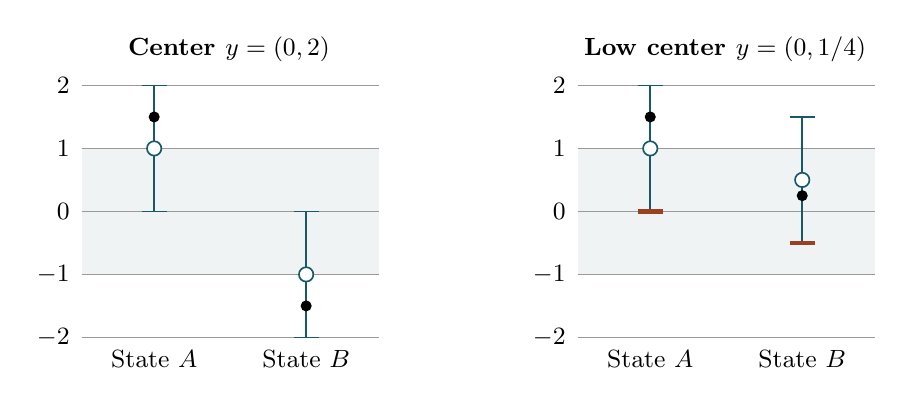
\begin{tikzpicture}[x=1cm,y=.80cm,font=\small,
  gridline/.style={black!40,thin},
  interval/.style={lagoon,semithick},
  guarantee/.style={ember,line width=1.6pt}]
\newcommand{\erroraxes}[1]{%
  \fill[lagoon!7] (.08,-1) rectangle (3.86,1);
  \foreach \k in {-2,-1,0,1,2}{
    \draw[gridline] (.08,\k)--(3.86,\k);
    \node[left] at (.05,\k){\(\k\)};
  }
  \node[anchor=south,font=\small\bfseries] at (1.95,2.22){#1};
  \node[below] at (1,-2.05){State \(A\)};
  \node[below] at (2.93,-2.05){State \(B\)};
}
\newcommand{\stateerror}[4]{%
  \draw[interval] (#1,{#2-1})--(#1,{#2+1});
  \draw[interval] ({#1-.16},{#2+1})--({#1+.16},{#2+1});
  \draw[#4] ({#1-.16},{#2-1})--({#1+.16},{#2-1});
  \draw[interval,fill=white] (#1,#2) circle[radius=2.6pt];
  \fill[black] (#1,#3) circle[radius=2pt];
}
\begin{scope}
  \erroraxes{Center \(y=(0,2)\)}
  \stateerror{1}{1}{1.5}{interval}
  \stateerror{2.93}{-1}{-1.5}{interval}
\end{scope}
\begin{scope}[xshift=6.3cm]
  \erroraxes{Low center \(y=(0,1/4)\)}
  \stateerror{1}{1}{1.5}{guarantee}
  \stateerror{2.93}{.5}{.25}{guarantee}
\end{scope}
\end{tikzpicture}
\caption{Clipped updates for the two-state game with \(H=1\).
The shaded band is the allowed range of the correction \(u\).
Each vertical interval is \([u_i-1,u_i+1]\), with the correction
at its open circle and the true error \(v_i-y_i\) at its solid dot.
In the right panel \(y<v\) in both states, so the lower endpoints
are certified policy guarantees relative to \(y\). Adding \(y\)
gives the absolute lower bound \(z=(0,-1/4)\).}
\label{fig:clip}
\end{figure}


\paragraph{Halving the width.}
The midpoint \(y=(L+U)/2\) has error at most \(W/2\). Apply the
clipped update three times with radii \(W/4,W/8,W/16\), replacing
\(y\) by \(y+u\) each time. By~\eqref{eq:dom} the resulting
\(y_*\) has error at most \(W/16\). Set \(H=W/8\). The lower estimate
\(y_*-H\mathbf1\) is strictly below \(v\) with error at most \(2H\),
so one more clipped solve gives a Max policy guaranteeing at least
\(v-(W/4)\mathbf1\). Likewise \(y_*+H\mathbf1\) gives a Min policy
guaranteeing at most \(v+(W/4)\mathbf1\). The two new MDP guarantees
thus have width at most \(W/2\).

\paragraph{The possible scales of a policy error.}
Halving alone gives an approximation. To get exact termination in
polynomially many iterations, we show that each positive width lies
within a factor \(2^{p(N)}\) of one of polynomially many positive
numbers, for a fixed polynomial \(p\). Here \(N\) is the length of the
discrete input, including the probability bits. The scales may depend
on the real input. The algorithm does not compute them.

Each of \(L,U\) is the payoff vector of a pair of policies, since a
best response in an MDP is positional and works from every state.
Moreover,
\[
   \max\{\|v-L\|_\infty,\|U-v\|_\infty\}\le W
      \le 2\max\{\|v-L\|_\infty,\|U-v\|_\infty\}.
\]
It therefore suffices to control the error of each policy pair. Write
\(\Delta\) for the vector of its payoffs minus \(v\) and suppose that
\(G=\|\Delta\|_\infty>0\). The \emph{action gaps}
\(\delta_a=r_a+B_a v-v_i\), defined for every action \(a\) at \(i\),
are common to all pairs. For the action used by the pair at \(i\),
\[
     \Delta_i=\delta_a+B_a\Delta .
\]
Thus \(g=\max_{a\ {\rm used}}|\delta_a|\le 2G\), and \(g>0\) by
contraction. When \(G\) is much larger than \(g\), the transition
chain must retain a large error across a whole closed set of states.

Indeed, change the signs of \(\Delta,\delta\) if necessary so that
some \(\Delta_i=G\). Write \(D_i=G-\Delta_i\). For the used action
\(a\) at \(i\),
\[
   \lambda_aG+B_aD=D_i+\delta_a\le D_i+g,\qquad
   P_aD\le 2(D_i+g).
\]
For the second inequality use \(D\le2G\mathbf1\) and
\((P_a-B_a)\mathbf1=\lambda_a\). Every positive transition has
probability at least \(2^{-\mathrm{poly}(N)}\). Along a transition
\(i\to j\), the last display bounds \(D_j\) by
\(2^{\mathrm{poly}(N)}(D_i+g)\). Each state reachable from a maximum
can be reached by a path of length at most \(n-1\). Starting with
\(D_i=0\) at the maximum, we obtain \(D_j\le Kg\) throughout its
reachable set for some uniform \(K=2^{\mathrm{poly}(N)}\).

If \(G\le2Kg\), the single gap of magnitude \(g\) supplies the scale.
Otherwise \(G/2\le\Delta_j\le G\) on the reachable set. This set is
closed under the undiscounted transitions of the pair. Choose a
stationary distribution supported there, assigning mass \(d_a\) to the
used action in each state. Such a distribution can be taken at a vertex
of the stationarity equations with nonnegative coordinates summing to
one. These equations use only transition probabilities, so every
positive \(d_a\) has polynomial bit length. Stationarity and the
recursion for \(\Delta\) give
\[
    \sum_a d_a\delta_a=\sum_a d_a(P_a-B_a)\Delta .
\]
The rows \(P_a-B_a\) are nonnegative, stay in the same reachable set,
and have masses \(\lambda_a\). Hence
\[
   (G/2)\sum_a d_a\lambda_a
   \le \sum_a d_a\delta_a\le G\sum_a d_a\lambda_a .
\]
The weighted discount loss \(\sum_a d_a\lambda_a\) is within a factor
\(2^{\mathrm{poly}(N)}\) of the largest \(\lambda_a\) in the support.
The numerator in the middle is a nonzero short rational combination
of the action gaps.

It remains to bound the number of scales for such numerators. Fix the
polynomial bit bound for their coefficient vectors. Take a maximal
collection of nonzero magnitudes of combinations of the gaps that
differ pairwise by factors greater than \(2^{p(N)}\), where \(p\) is
chosen below. By maximality each nonzero magnitude is within that
factor of one in the collection. The selected coefficient vectors are
linearly independent. Indeed, any dependence contains a dependence on
at most \(m+1\) vectors, where \(m\) is the number of actions. Clearing
denominators and applying determinant bounds gives integer dependence
coefficients of \(\ell_1\)-norm less than \(2^{p(N)}\) for a
sufficiently large fixed polynomial \(p\). Applying that dependence to
the combination values gives a contradiction. The term of largest
magnitude among the values with nonzero coefficient exceeds the sum of
the magnitudes of all smaller terms even after weighting by their
coefficients.

There are at most \(m\) numerator scales. For \(G>2Kg\), divide one
of them by one of the \(m\) discount losses \(\lambda_a\). For
\(G\le2Kg\), use one of the \(m\) individual gap magnitudes. After
increasing \(p\) to absorb the comparison factors, these at most
\(m^2+m\) scales work for every pair, hence for every positive \(W\).
A sequence of successive halvings has at most \(2p(N)+1\) widths
in the interval from \(2^{-p(N)}\) to \(2^{p(N)}\) times any one scale.
The algorithm therefore reaches \(W=0\) after polynomially many
iterations.

\paragraph{Arithmetic and parameter dependence.}
Only the two discrete policies pass between iterations. Within each
iteration a constant number of MDP evaluations and clipped solves
suffice. The step count is polynomial in \(N\), and the bit bounds of
Section~\ref{sec:arithmetic} apply to each iteration.

Finally let the rewards and discounts be polynomials in \(t\), valid
for all sufficiently small positive \(t\). Their degrees count in the
input size, and the probabilities are fixed binary rationals. The MDP
algorithm of Section~\ref{sec:mdp} returns best responses and
guarantees as rational functions. Compare two such functions using
their signs at \(0^+\), so the policy selections hold throughout a
sufficiently small positive interval.

In a clipped solve the height \(H\) and offsets
\(c_a=r_a+B_a y-y_i\) are now rational functions. Choose a common
denominator \(d\), positive near \(0^+\), so that \(dH\) and every
\(dc_a\) are polynomials. Let \(K>0\) bound \(|dH|\) on \(0<t<1\),
for example one plus the sum of the absolute values of its
coefficients. In the scaled coordinates \(\xi=du/K\), Equation
\eqref{eq:clip} has offsets \(dc_a/K\), rows \(P_a\), and clipping
endpoints \(\pm dH/K\). These endpoints lie in \([-1,1]\) near
\(0^+\). The resulting nonexpansive map of the unit cube fits
Proposition~\ref{prop:asym}, which yields a rational \(\xi\) and the
required extremizing actions. Recover \(u=K\xi/d\).

Degrees remain polynomial because each iteration has a constant number
of layers of calls, and passes only policies to the next iteration.
Products and sums of polynomially many polynomials of these degrees
can be computed by evaluation and interpolation using polynomial-size
formulas in their coefficients, as required in
Section~\ref{sec:arithmetic}. Every finite sequence of symbolic
iterations agrees with a run at a common sufficiently small \(t>0\).
The pointwise iteration bound is uniform in \(t\), so the symbolic
algorithm has the same bound. Applied to~\eqref{eq:gz}, it supplies
Blackwell optimal policies even for arbitrary positive real weights.
The mean-payoff limit of Section~\ref{sec:shortslopes} completes the
proof of Theorem~\ref{thm:games}.

\section{Tropical feasibility and further questions}\label{sec:closing}

The prices in the LP algorithm enter a comparison by addition to a logarithmic
magnitude. A system of tropical linear inequalities makes such comparisons
directly. Akian, Gaubert and Guterman~\cite{AGG} related its feasibility
to the values of a mean-payoff game (see also~\cite{MSS,DG}).
Theorem~\ref{thm:games} thus gives one further algorithmic consequence.

\begin{corollary}[Tropical linear feasibility]\label{cor:tropical}
Let \(a_{ri},b_{ri}\) be explicitly given entries in
\(\RR\cup\{-\infty\}\) of two \(m\times n\) matrices.
For the system
\[
                \max_i(a_{ri}+x_i)\ \le\ \max_j(b_{rj}+x_j)
                  \qquad\text{for every row \(r\)},
\]
a deterministic strongly polynomial algorithm finds a solution in
\((\RR\cup\{-\infty\})^n\) finite at every coordinate that can be
finite in any solution. An empty maximum equals \(-\infty\).
\end{corollary}

\begin{proof}
Use the game of~\cite{AGG}. At coordinate \(i\), Min may choose any row
\(r\) with \(a_{ri}\) finite. At row \(r\), Max may choose any coordinate
\(j\) with \(b_{rj}\) finite. The two successive edges have rewards
\(-a_{ri}\) and \(b_{rj}\). Give a vertex with no move a self-loop of
reward zero if it belongs to Min, and of reward \(-1\) if it belongs to Max.

A coordinate \(i\) finite in a solution has nonnegative game value.
After Min chooses a row there, Max takes a term attaining the right-hand
maximum. Its coordinate \(j\) is finite and
\(-a_{ri}+b_{rj}\ge x_i-x_j\). Summing over the play telescopes.
The finite coordinates form a finite set, so the bounded endpoint
contribution vanishes in the mean payoff.

Conversely, compute the values and fix an optimal policy for Max by
Theorem~\ref{thm:games}. From a coordinate of nonnegative value, Min can
reach no negative-weight cycle under this policy, since Min could then
repeat the cycle. In particular, every reachable Max vertex has a move
in the original game. At each coordinate reachable from a nonnegative-value
start, set \(x_i\) to the least total weight of a walk starting at \(i\)
with Max's policy fixed, allowing the empty walk. Erasing cycles shows
that a simple walk attains the minimum. At all other coordinates put
\(x_i=-\infty\). For each permitted pair of moves \(i,r,j\) from a
finite coordinate, concatenating the two moves with a minimizing walk
from \(j\) gives \(x_i\le -a_{ri}+b_{rj}+x_j\). Hence the row
inequalities hold. Dynamic programming over walks of length at most
the number of vertices computes the minima in strongly polynomial time.
\end{proof}

A constant term in a maximum can be homogenized by adding one coordinate.
The original system is feasible precisely when this coordinate can be finite.
In that case subtract its value from every coordinate to recover a solution.

\paragraph{Further questions.}
Allamigeon, Benchimol, Gaubert and Joswig~\cite{ABGJgame} showed how a
strongly polynomial combinatorial simplex algorithm could yield strongly
polynomial time for mean-payoff games. The algorithm of Theorem~\ref{thm:lp}
uses quantitative comparisons of minors as well as their signs. Some
comparisons in Section~\ref{sec:compression} have degree exponential in
the dimensions. Can a strongly polynomial LP algorithm use predicates of
polynomial degree throughout?

Theorem~\ref{thm:lp} takes the constraints as explicit input. For a
polyhedron given by a separation oracle, known exact algorithms also
involve geometric parameters~\cite{DVZ26}. A further question concerns
transition probabilities in games. Theorem~\ref{thm:games} permits
arbitrary real probabilities for one player. For two players its step
bound still depends on the bit lengths of the probabilities.
Can that dependence be removed?

\begin{thebibliography}{150}
\small
\addcontentsline{toc}{section}{References}

\bibitem{AGG}
M. Akian, S. Gaubert, and A. Guterman, \emph{Tropical polyhedra are equivalent to mean payoff games}, Internat. J. Algebra Comput. \textbf{22} (2012), \texttt{doi:10.1142/S0218196711006674}.

\bibitem{ABGJgame}
X. Allamigeon, P. Benchimol, S. Gaubert, and M. Joswig, \emph{Combinatorial simplex algorithms can solve mean payoff games}, SIAM J. Optim. \textbf{24} (2014), 2096--2117.

\bibitem{ABGJ}
X. Allamigeon, P. Benchimol, S. Gaubert, and M. Joswig, \emph{Log-barrier interior point methods are not strongly polynomial}, SIAM J. Appl. Algebra Geom. \textbf{2} (2018), 140--178.

\bibitem{AGKS}
X. Allamigeon, S. Gaubert, R. D. Katz, and M. Skomra, \emph{Universal complexity bounds based on value iteration for stochastic mean payoff games and entropy games}, Inform. and Comput. \textbf{302} (2025), 105236.

\bibitem{AGV}
X. Allamigeon, S. Gaubert, and N. Vandame, \emph{No self-concordant barrier interior point method is strongly polynomial}, Proc. STOC 2022, 515--528.

\bibitem{AM}
D. Andersson and P. B. Miltersen, \emph{The complexity of solving stochastic games on graphs}, Proc. ISAAC 2009, 112--121.

\bibitem{AHK}
S. Arora, E. Hazan, and S. Kale, \emph{The multiplicative weights update method: a meta-algorithm and applications}, Theory Comput. \textbf{8} (2012), 121--164.

\bibitem{Awon}
S. Awoniyi, \emph{A strongly polynomial-time algorithm for the general linear programming problem}, arXiv:2503.12041 (2025; revised 2026).

\bibitem{BH}
E. Bach and S. Huiberts, \emph{Optimal smoothed analysis of the simplex method}, Proc. FOCS 2025, 1829--1856.

\bibitem{Ban}
S. Banach, \emph{Sur les op\'erations dans les ensembles abstraits et leur application aux \'equations int\'egrales}, Fund. Math. \textbf{3} (1922), 133--181.

\bibitem{BFGMS}
E. Batziou, J. Fearnley, S. Gordon, R. Mehta, and R. Savani, \emph{Monotone contractions}, Proc. STOC 2025, 507--517.

\bibitem{BELL}
R. Bellman, \emph{Dynamic programming}, Princeton Univ. Press, 1957.

\bibitem{Betke}
U. Betke, \emph{Relaxation, new combinatorial and polynomial algorithms for the linear feasibility problem}, Discrete Comput. Geom. \textbf{32} (2004), 317--338.

\bibitem{BSV}
H. Bj\"orklund, S. Sandberg, and S. Vorobyov, \emph{A combinatorial strongly subexponential strategy improvement algorithm for mean payoff games}, Proc. MFCS 2004, 673--685.

\bibitem{BV}
H. Bj\"orklund and S. Vorobyov, \emph{A combinatorial strongly subexponential strategy improvement algorithm for mean payoff games}, Discrete Appl. Math. \textbf{155} (2007), 210--229.

\bibitem{Black}
D. Blackwell, \emph{An analog of the minimax theorem for vector payoffs}, Pacific J. Math. \textbf{6} (1956), 1--8.

\bibitem{Bla}
D. Blackwell, \emph{Discrete dynamic programming}, Ann. Math. Statist. \textbf{33} (1962), 719--726.

\bibitem{BSS}
L. Blum, M. Shub, and S. Smale, \emph{On a theory of computation and complexity over the real numbers: NP-completeness, recursive functions and universal machines}, Bull. Amer. Math. Soc. (N.S.) \textbf{21} (1989), 1--46.

\bibitem{BEGM}
E. Boros, K. Elbassioni, V. Gurvich, and K. Makino, \emph{A pseudo-polynomial algorithm for mean payoff stochastic games with perfect information and few random positions}, Inform. and Comput. \textbf{267} (2019), 74--95.

\bibitem{Boyd}
S. Boyd and L. Vandenberghe, \emph{Convex Optimization}, Cambridge University Press, 2004.

\bibitem{BC}
Lubo\v{s} Brim, J. Chaloupka, L. Doyen, R. Gentilini, and J.-F. Raskin, \emph{Faster algorithms for mean-payoff games}, Formal Methods System Design \textbf{38} (2011), 97--118.

\bibitem{Cal}
C. S. Calude, S. Jain, B. Khoussainov, W. Li, and F. Stephan, \emph{Deciding parity games in quasi-polynomial time}, SIAM J. Comput. \textbf{51} (2022), STOC17-152--STOC17-188.

\bibitem{CLY}
X. Chen, Y. Li, and M. Yannakakis, \emph{Computing a fixed point of contraction maps in polynomial queries}, J.~ACM \textbf{72} (2025), Art.~25.

\bibitem{CLYsp}
X. Chen, Y. Li, and M. Yannakakis, \emph{Quadratic speedup for computing contraction fixed points}, arXiv:2602.10296 (2026).

\bibitem{CLYdec}
X. Chen, Y. Li, and M. Yannakakis, \emph{A decomposition theorem and a simple algorithm for contraction fixed points}, arXiv:2611.01302 (2026).

\bibitem{Chu}
S. Chubanov, \emph{A polynomial projection algorithm for linear feasibility problems}, Math. Program. \textbf{153} (2015), 687--713.

\bibitem{CLS}
M. B. Cohen, Y. T. Lee, and Z. Song, \emph{Solving linear programs in the current matrix multiplication time}, Proc. STOC 2019, 938--942.

\bibitem{Cond}
A. Condon, \emph{The complexity of stochastic games}, Inform. and Comput. \textbf{96} (1992), 203--224.

\bibitem{Cottle}
R. W. Cottle, \emph{Note on a fundamental theorem in quadratic programming}, J. Soc. Indust. Appl. Math. \textbf{12} (1964), 663--665.

\bibitem{CD}
R. W. Cottle and G. B. Dantzig, \emph{Complementary pivot theory of mathematical programming}, Linear Algebra Appl. \textbf{1} (1968), 103--125.

\bibitem{CPS}
R. W. Cottle, J.-S. Pang, and R. E. Stone, \emph{The Linear Complementarity Problem}, Academic Press, 1992.

\bibitem{CLM}
B. Cui, H. Li, and X. Miao, \emph{Extending Tardos's theorem to separable convex quadratic programming}, arXiv:2610.07465v2 (2026).

\bibitem{DHNV}
D. Dadush, S. Huiberts, B. Natura, and L. A. V\'egh, \emph{A scaling-invariant algorithm for linear programming whose running time depends only on the constraint matrix}, Math. Program. \textbf{204} (2024), 135--206.

\bibitem{DKNOV}
D. Dadush, Z. K. Koh, B. Natura, N. Olver, and L. A. V\'egh, \emph{A strongly polynomial algorithm for linear programs with at most two nonzero entries per row or column}, Proc. STOC 2024, 1561--1572.

\bibitem{DKNOV26}
D. Dadush, Z. K. Koh, B. Natura, N. Olver, and L. A. V\'egh, \emph{Solving classes of linear programs with strongly polynomial straight line complexity in strongly polynomial time}, arXiv:2610.26073 (2026).

\bibitem{Newton}
D. Dadush, Z. K. Koh, B. Natura, and L. A. V\'egh, \emph{An accelerated Newton--Dinkelbach method and its application to two variables per inequality systems}, Math. Oper. Res. \textbf{48} (2023), 1934--1958; arXiv:2004.08634.

\bibitem{DNV}
D. Dadush, B. Natura, and L. A. V\'egh, \emph{Revisiting Tardos's framework for linear programming: Faster exact solutions using approximate solvers}, Proc. FOCS 2020, 931--942.

\bibitem{DVZ}
D. Dadush, L. A. V\'egh, and G. Zambelli, \emph{Rescaling algorithms for linear conic feasibility}, arXiv:1611.06427 (2016; revised 2019).

\bibitem{DVZ26}
D. Dadush, L. A. V\'egh, and G. Zambelli, \emph{On finding exact solutions of linear programs in the oracle model}, arXiv:2606.11820 (2026; conference version, SODA 2022).

\bibitem{Dantzig}
G. B. Dantzig, \emph{Maximization of a linear function of variables subject to linear inequalities}, Activity Analysis of Production and Allocation (T.~C. Koopmans, ed.), Cowles Commission Monograph~13, Wiley, 1951, 339--347.

\bibitem{DFZ}
C. Daskalakis, G. Farina, and B. H. Zhang, \emph{Polynomial-time computation of \(\ell_p\)-contraction fixed points for even \(p\)}, arXiv:2607.23863 (2026).

\bibitem{DP}
C. Daskalakis and C. H. Papadimitriou, \emph{Continuous local search}, Proc. SODA 2011, 790--804.

\bibitem{AHM}
L. de Alfaro, T.~A. Henzinger, and R. Majumdar, \emph{Discounting the future in systems theory}, Proc. ICALP 2003, 1022--1037.

\bibitem{DLHR}
J. A. De Loera, J. Haddock, and L. Rademacher, \emph{The minimum Euclidean-norm point in a convex polytope: Wolfe's combinatorial algorithm is exponential}, SIAM J. Comput. \textbf{49} (2020), 138--169.

\bibitem{Dpen}
F. d'Epenoux, \emph{A probabilistic production and inventory problem}, Management Sci. \textbf{10} (1963), 98--108.

\bibitem{DG}
V. Dhingra and S. Gaubert, \emph{How to solve large scale deterministic games with mean payoff by policy iteration}, Proc. VALUETOOLS 2006, Art.~12.

\bibitem{DV}
J. Dunagan and S. Vempala, \emph{A simple polynomial-time rescaling algorithm for solving linear programs}, Math. Program. \textbf{114} (2008), 101--114.

\bibitem{EK}
D. Easley and J. Kleinberg, \emph{Networks, crowds, and markets: reasoning about a highly connected world}, Cambridge Univ. Press, 2010.

\bibitem{EM}
A. Ehrenfeucht and J. Mycielski, \emph{Positional strategies for mean payoff games}, Internat. J. Game Theory \textbf{8} (1979), 109--113.

\bibitem{CIRC}
F. Ekbatani, B. Natura, and L. A. V\'egh, \emph{Circuit imbalance measures and linear programming}, Surveys in Combinatorics 2022, Cambridge Univ. Press, 64--114.

\bibitem{EPRY}
K. Etessami, C. H. Papadimitriou, A. Rubinstein, and M. Yannakakis, \emph{Tarski's theorem, supermodular games, and the complexity of equilibria}, Proc. ITCS 2020 (LIPIcs \textbf{151}), 18:1--18:19.

\bibitem{EY}
K. Etessami and M. Yannakakis, \emph{On the complexity of Nash equilibria and other fixed points}, SIAM J. Comput. \textbf{39} (2010), 2531--2597.

\bibitem{Fark}
J. Farkas, \emph{Theorie der einfachen Ungleichungen}, J. Reine Angew. Math. \textbf{124} (1902), 1--27.

\bibitem{FGMS}
J. Fearnley, S. Gordon, R. Mehta, and R. Savani, \emph{Unique end of potential line}, J. Comput. System Sci. \textbf{114} (2020), 1--35.

\bibitem{FH}
A. Feodorov and S. Haslebacher, \emph{Faster approximate fixed points of \(\ell_\infty\)-contractions}, arXiv:\allowbreak 2604.01006 (2026).

\bibitem{FAA}
J. A. Filar, E. Altman, and K. E. Avrachenkov, \emph{An asymptotic simplex method for singularly perturbed linear programs}, Oper. Res. Lett. \textbf{30} (2002), 295--307.

\bibitem{FT}
A. Frank and \'{E}. Tardos, \emph{An application of simultaneous Diophantine approximation in combinatorial optimization}, Combinatorica \textbf{7} (1987), 49--65.

\bibitem{FW}
M. Frank and P. Wolfe, \emph{An algorithm for quadratic programming}, Naval Res. Logist. Quart. \textbf{3} (1956), 95--110.

\bibitem{FS}
Y. Freund and R. E. Schapire, \emph{A decision-theoretic generalization of on-line learning and an application to boosting}, J. Comput. System Sci. \textbf{55} (1997), 119--139.

\bibitem{FKV}
S. Fujishige, T. Kitahara, and L. A. V\'egh, \emph{An update-and-stabilize framework for the minimum-norm-point problem}, Math. Program. \textbf{210} (2025), 281--311.

\bibitem{Gale}
D. Gale, H. W. Kuhn, and A. W. Tucker, \emph{Linear programming and the theory of games}, in Activity Analysis of Production and Allocation (T. C. Koopmans, ed.), Wiley, 1951, 317--335.

\bibitem{GR}
B. G\"artner and L. Y. R\"ust, \emph{Simple stochastic games and P-matrix generalized linear complementarity problems}, Proc. FCT 2005, 209--220.

\bibitem{GGK}
S. Gaubert, J. Grand-Cl\'ement, and R. D. Katz, \emph{Thresholds for sensitive optimality and Blackwell optimality in stochastic games}, Advances in Neural Information Processing Systems 38, 2025.

\bibitem{GPV}
M. Ghadiri, R. Peng, and S. S. Vempala, \emph{The bit complexity of efficient continuous optimization}, Proc. FOCS 2023, 2059--2070.

\bibitem{Gillet}
D. Gillette, \emph{Stochastic games with zero stop probabilities}, Contributions to the Theory of Games, Vol.~III (M.~Dresher, A.~W. Tucker, and P.~Wolfe, eds.), Princeton Univ. Press, 1957, 179--187.

\bibitem{GZDet}
H. Gimbert and W. Zielonka, \emph{Deterministic priority mean-payoff games as limits of discounted games}, Proc. ICALP 2006 (II), 312--323.

\bibitem{GZMD}
H. Gimbert and W. Zielonka, \emph{Limits of multi-discounted Markov decision processes}, Proc. LICS 2007, 89--98.

\bibitem{GZ}
H. Gimbert and W. Zielonka, \emph{Blackwell-optimal strategies in priority mean-payoff games}, Electron. Proc. Theor. Comput. Sci. \textbf{25} (2010), 7--21.

\bibitem{GT}
A. J. Goldman and A. W. Tucker, \emph{Theory of linear programming}, in Linear Inequalities and Related Systems (H. W. Kuhn and A. W. Tucker, eds.), Annals of Mathematics Studies~38, Princeton Univ. Press, 1956.

\bibitem{GSK}
F. Granot and J. Skorin-Kapov, \emph{Towards a strongly polynomial algorithm for strictly convex quadratic programs: an extension of Tardos' algorithm}, Math. Programming \textbf{46} (1990), 225--236.

\bibitem{GLS}
M. Gr\"otschel, L. Lov\'asz, and A. Schrijver, \emph{Geometric algorithms and combinatorial optimization}, Algorithms and Combinatorics~2, Springer, 1988.

\bibitem{GKK}
V. A. Gurvich, A. V. Karzanov, and L. G. Khachiyan, \emph{Cyclic games and an algorithm to find minimax cycle means in directed graphs}, USSR Comput. Math. and Math. Phys. \textbf{28} (1988), 85--91.

\bibitem{Hal}
N. Halman, \emph{Simple stochastic games, parity games, mean payoff games and discounted payoff games are all LP-type problems}, Algorithmica \textbf{49} (2007), 37--50.

\bibitem{HIJ}
T. D. Hansen and R. Ibsen-Jensen, \emph{The complexity of interior point methods for solving discounted turn-based stochastic games}, arXiv:1304.1888v2 (2014).

\bibitem{HMZ}
T. D. Hansen, P. B. Miltersen, and U. Zwick, \emph{Strategy iteration is strongly polynomial for 2-player turn-based stochastic games with a constant discount factor}, J.~ACM \textbf{60} (2013), Art.~1.

\bibitem{HZ}
T. D. Hansen and U. Zwick, \emph{An improved version of the Random-Facet pivoting rule for the simplex algorithm}, Proc. STOC 2015, 209--218.

\bibitem{HLSW}
S. Haslebacher, J. Lill, P. Schnider, and S. Weber, \emph{Query-efficient fixpoints of \(\ell_p\)-contractions}, Proc. FOCS 2025, 2037--2053.

\bibitem{HV}
S.-P. Hong and S. Verma, \emph{A note on the strong polynomiality of convex quadratic programming}, Math. Programming \textbf{68} (1995), 131--139.

\bibitem{HOW}
R. A. Howard, \emph{Dynamic programming and Markov processes}, MIT Press, 1960.

\bibitem{HKS}
Z. Huang, L. Khachiyan, and K. Sikorski, \emph{Approximating fixed points of weakly contracting mappings}, J. Complexity \textbf{15} (1999), 200--213.

\bibitem{Jero}
R. G. Jeroslow, \emph{Asymptotic linear programming}, Oper. Res. \textbf{21} (1973), 1128--1141.

\bibitem{Jur}
M. Jurdzi\'nski, \emph{Deciding the winner in parity games is in UP \(\cap\) co-UP}, Inform. Process. Lett. \textbf{68} (1998), 119--124.

\bibitem{JSav}
M. Jurdzi\'nski and R. Savani, \emph{A simple P-matrix linear complementarity problem for discounted games}, in Proc. CiE 2008, 283--293.

\bibitem{Kalai}
G. Kalai, \emph{A subexponential randomized simplex algorithm} (extended abstract), Proc. STOC 1992, 475--482.

\bibitem{KK}
G. Kalai and D. J. Kleitman, \emph{A quasi-polynomial bound for the diameter of graphs of polyhedra}, Bull. Amer. Math. Soc. (N.S.) \textbf{26} (1992), 315--316.

\bibitem{Kan}
L. V. Kantorovich, \emph{Mathematical methods of organizing and planning production}, Management Sci. \textbf{6} (1960), 366--422 (translation; Russian original, 1939).

\bibitem{Kar}
N. Karmarkar, \emph{A new polynomial-time algorithm for linear programming}, Combinatorica \textbf{4} (1984), 373--395.

\bibitem{Khach}
L. G. Khachiyan, \emph{A polynomial algorithm in linear programming} (Russian), Dokl. Akad. Nauk SSSR \textbf{244} (1979), 1093--1096.

\bibitem{Khach2}
L. G. Khachiyan, \emph{Polynomial algorithms in linear programming} (Russian), Zh. Vychisl. Mat. Mat. Fiz. \textbf{20} (1980), 51--68.

\bibitem{KM}
V. Klee and G. J. Minty, \emph{How good is the simplex algorithm?} Inequalities~III (O.~Shisha, ed.), Academic Press, 1972, 159--175.

\bibitem{KMY}
M. Kojima, S. Mizuno, and A. Yoshise, \emph{A polynomial-time algorithm for a class of linear complementarity problems}, Math. Programming \textbf{44} (1989), 1--26.

\bibitem{KTK}
M. K. Kozlov, S. P. Tarasov, and L. G. Khachiyan, \emph{The polynomial solvability of convex quadratic programming}, Zh. Vychisl. Mat. Mat. Fiz. \textbf{20} (1980), 1319--1323 (in Russian).

\bibitem{KuhHist}
H. W. Kuhn, \emph{Nonlinear programming. A historical view}, in Nonlinear Programming (R. W. Cottle and C. E. Lemke, eds.), SIAM--AMS Proc. 9, AMS, 1976, 1--26.

\bibitem{KT}
H. W. Kuhn and A. W. Tucker, \emph{Nonlinear programming}, in Proc. Second Berkeley Symp. Math. Statist. Probab., University of California Press, 1951, 481--492.

\bibitem{LLL}
A. K. Lenstra, H. W. Lenstra, Jr., and L. Lov\'asz, \emph{Factoring polynomials with rational coefficients}, Math. Ann. \textbf{261} (1982), 515--534.

\bibitem{LY}
V. F. Lev and R. Yuster, \emph{On the size of dissociated bases}, arXiv:1005.0155 (2010).

\bibitem{LL}
T. M. Liggett and S. A. Lippman, \emph{Stochastic games with perfect information and time average payoff}, SIAM Rev. \textbf{11} (1969), 604--607.

\bibitem{Litt}
N. Littlestone and M. K. Warmuth, \emph{The weighted majority algorithm}, Inform. and Comput. \textbf{108} (1994), 212--261.

\bibitem{Lobo}
M. S. Lobo, L. Vandenberghe, S. Boyd, and H. Lebret, \emph{Applications of second-order cone programming}, Linear Algebra Appl. \textbf{284} (1998), 193--228.

\bibitem{Lud}
W. Ludwig, \emph{A subexponential randomized algorithm for the simple stochastic game problem}, Inform. and Comput. \textbf{117} (1995), 151--155.

\bibitem{Man}
O.~L. Mangasarian, \emph{A simple characterization of solution sets of convex programs}, Oper. Res. Lett. \textbf{7} (1988), 21--26.

\bibitem{MSW}
J. Matou\v{s}ek, M. Sharir, and E. Welzl, \emph{A subexponential bound for linear programming}, Algorithmica \textbf{16} (1996), 498--516.

\bibitem{McSh}
E. J. McShane, \emph{Extension of range of functions}, Bull. Amer. Math. Soc. \textbf{40} (1934), 837--842.

\bibitem{MegEnc}
N. Megiddo, \emph{Is binary encoding appropriate for the problem-language relationship?} Theoret. Comput. Sci. \textbf{19} (1982), 337--341.

\bibitem{Meg}
N. Megiddo, \emph{Towards a genuinely polynomial algorithm for linear programming}, SIAM J. Comput. \textbf{12} (1983), 347--353.

\bibitem{MegLin}
N. Megiddo, \emph{Linear programming in linear time when the dimension is fixed}, J. ACM \textbf{31} (1984), 114--127.

\bibitem{MSS}
R. H. M\"ohring, M. Skutella, and F. Stork, \emph{Scheduling with AND/OR precedence constraints}, SIAM J. Comput. \textbf{33} (2004), 393--415.

\bibitem{Natura}
B. Natura, \emph{Circuit diameter of polyhedra is strongly polynomial}, arXiv:2602.06958 (2026).

\bibitem{NN}
Y. Nesterov and A. Nemirovskii, \emph{Interior-point polynomial algorithms in convex programming}, SIAM, 1994.

\bibitem{Ohl}
P. Ohlmann, \emph{A symmetric recursive algorithm for mean-payoff games}, arXiv:2603.07555 (2026).

\bibitem{OV}
N. Olver and L. A. V\'egh, \emph{A simpler and faster strongly polynomial algorithm for generalized flow maximization}, J. ACM \textbf{67} (2020), Art.~10.

\bibitem{OAIDe}
{\raggedright OpenAI, \emph{Deterministic quasipolynomial-time mean-payoff games},
OpenAI Math Release preprint
\href{https://github.com/openai/math/blob/main/preprints/Deterministic-quasipolynomial-time-mean-payoff-games-September-25-2026/paper.pdf}{{\ttfamily OAI:Deterministic-\allowbreak{}quasipolynomial-\allowbreak{}time-\allowbreak{}mean-\allowbreak{}payoff-\allowbreak{}games-\allowbreak{}September-\allowbreak{}25-\allowbreak{}2026}}, 2026.\par}

\bibitem{OAIRa}
{\raggedright OpenAI, \emph{Randomized quasipolynomial-time mean-payoff games},
OpenAI Math Release preprint
\href{https://github.com/openai/math/blob/main/preprints/Randomized-quasipolynomial-time-mean-payoff-games-September-25-2026/paper.pdf}{{\ttfamily OAI:Randomized-\allowbreak{}quasipolynomial-\allowbreak{}time-\allowbreak{}mean-\allowbreak{}payoff-\allowbreak{}games-\allowbreak{}September-\allowbreak{}25-\allowbreak{}2026}}, 2026.\par}

\bibitem{OAITu}
{\raggedright OpenAI, \emph{Turn-Based Stochastic Mean-Payoff Games in Deterministic Quasipolynomial Time},
OpenAI Math Release preprint
\href{https://github.com/openai/math/blob/main/preprints/Turn-Based-Stochastic-Mean-Payoff-Games-in-Deterministic-Quasipolynomial-Time-October-5-2026/stochastic-mean-payoff-games.pdf}{{\ttfamily OAI:Turn-\allowbreak{}Based-\allowbreak{}Stochastic-\allowbreak{}Mean-\allowbreak{}Payoff-\allowbreak{}Games-\allowbreak{}in-\allowbreak{}Deterministic-\allowbreak{}Quasipolynomial-\allowbreak{}Time-\allowbreak{}October-\allowbreak{}5-\allowbreak{}2026}}, 2026.\par}

\bibitem{OAIMe}
{\raggedright OpenAI, \emph{Mean-payoff parity games in quasipolynomial time},
OpenAI Math Release preprint
\href{https://github.com/openai/math/blob/main/preprints/Mean-payoff-parity-games-in-quasipolynomial-time-October-5-2026/mean-payoff-parity.pdf}{{\ttfamily OAI:Mean-\allowbreak{}payoff-\allowbreak{}parity-\allowbreak{}games-\allowbreak{}in-\allowbreak{}quasipolynomial-\allowbreak{}time-\allowbreak{}October-\allowbreak{}5-\allowbreak{}2026}}, 2026.\par}

\bibitem{OAIHirsch}
{\raggedright OpenAI, \emph{Superpolynomial graph diameter of simple polytopes},
OpenAI Math Release preprint
\href{https://github.com/openai/math/blob/main/preprints/Superpolynomial-graph-diameter-of-simple-polytopes-November-24-2026/paper.pdf}{{\ttfamily OAI:Superpolynomial-\allowbreak{}graph-\allowbreak{}diameter-\allowbreak{}of-\allowbreak{}simple-\allowbreak{}polytopes-\allowbreak{}November-\allowbreak{}24-\allowbreak{}2026}}, 2026.\par}

\bibitem{Parys}
P. Parys, \emph{Parity games: Zielonka's algorithm in quasi-polynomial time}, Proc. MFCS 2019, LIPIcs~138, 10:1--10:13.

\bibitem{PS}
J. Pe\~na and N. Soheili, \emph{Projection and rescaling algorithm for finding maximum support solutions to polyhedral conic systems}, Math. Oper. Res. \textbf{47} (2022), 3304--3316.

\bibitem{PY}
I. Post and Y. Ye, \emph{The simplex method is strongly polynomial for deterministic Markov decision processes}, Math. Oper. Res. \textbf{40} (2015), 859--868.

\bibitem{Puri}
A. Puri, \emph{Theory of hybrid systems and discrete event systems}, Ph.D.\ thesis, University of California at Berkeley, 1995.

\bibitem{PUT}
M. L. Puterman, \emph{Markov decision processes: discrete stochastic dynamic programming}, Wiley, 1994.

\bibitem{Rad}
T. Radzik, \emph{Fractional combinatorial optimization}, Handbook of Combinatorial Optimization (D.-Z. Du and P.~M. Pardalos, eds.), 1998, 429--478.

\bibitem{Ren}
J. Renegar, \emph{A polynomial-time algorithm, based on Newton's method, for linear programming}, Math. Program. \textbf{40} (1988), 59--93.

\bibitem{Rock}
R. T. Rockafellar, \emph{The elementary vectors of a subspace of \(\mathbb R^N\)}, Combinatorial Mathematics and Its Applications (R.~C. Bose and T.~A. Dowling, eds.), Univ. of North Carolina Press, 1969, 104--127.

\bibitem{Santos}
F. Santos, \emph{A counterexample to the Hirsch conjecture}, Ann. of Math. (2) \textbf{176} (2012), 383--412.

\bibitem{Shap}
L. S. Shapley, \emph{Stochastic games}, Proc. Natl. Acad. Sci. USA \textbf{39} (1953), 1095--1100.

\bibitem{Sik}
S. Shellman and K. Sikorski, \emph{A recursive algorithm for the infinity-norm fixed point problem}, J. Complexity \textbf{19} (2003), 799--834.

\bibitem{Shor}
N. Z. Shor, \emph{Cut-off method with space extension in convex programming problems} (Russian), Kibernetika (Kiev) (1977), no.~1, 94--95.

\bibitem{STWon}
K. Sikorski, C.-W. Tsay, and H. Wo\'zniakowski, \emph{An ellipsoid algorithm for the computation of fixed points}, J. Complexity \textbf{9} (1993), 181--200.

\bibitem{Smale}
S. Smale, \emph{Mathematical problems for the next century}, Math. Intelligencer \textbf{20} (1998), no.~2, 7--15.

\bibitem{SF}
A. Soleymani and G. Farina, \emph{A quasipolynomial algorithm for \(\ell_\infty\) contractions}, arXiv:2610.30122 (2026).

\bibitem{ST}
D. A. Spielman and S.-H. Teng, \emph{Smoothed analysis of algorithms: Why the simplex algorithm usually takes polynomial time}, J. ACM \textbf{51} (2004), 385--463.

\bibitem{TarCirc}
\'{E}. Tardos, \emph{A strongly polynomial minimum cost circulation algorithm}, Combinatorica \textbf{5} (1985), 247--255.

\bibitem{Tardos}
\'{E}. Tardos, \emph{A strongly polynomial algorithm to solve combinatorial linear programs}, Oper. Res. \textbf{34} (1986), 250--256.

\bibitem{Tari}
R. E. Tarjan, \emph{Efficient algorithms for network optimization}, in Proc. ICM 1983, vol.~2, PWN/North-Holland, 1984, 1619--1635.

\bibitem{Tru1}
L. Truffet, \emph{Looking for all solutions of a set of max-atoms solves the max atom problem in strongly polynomial time}, Mod\'elisation des Syst\`emes R\'eactifs (MSR~2025), hal-05491586, 2025.

\bibitem{Tru2}
L. Truffet, \emph{Substitution for minimizing/maximizing a tropical linear (fractional) programming}, arXiv:2603.26423 (2026).

\bibitem{Tuc}
A. W. Tucker, \emph{Dual systems of homogeneous linear relations}, in Linear Inequalities and Related Systems (H. W. Kuhn and A. W. Tucker, eds.), Annals of Mathematics Studies~38, Princeton Univ. Press, 1956, 3--18.

\bibitem{Vai}
P. M. Vaidya, \emph{Speeding-up linear programming using fast matrix multiplication} (extended abstract), Proc. FOCS 1989, 332--337.

\bibitem{VDB}
J. van den Brand, \emph{A deterministic linear program solver in current matrix multiplication time}, Proc. SODA 2020, 259--278.

\bibitem{VY}
S. A. Vavasis and Y. Ye, \emph{A primal-dual interior point method whose running time depends only on the constraint matrix}, Math. Program. \textbf{74} (1996), 79--120.

\bibitem{VQ}
L. A. V\'egh, \emph{A strongly polynomial algorithm for a class of minimum-cost flow problems with separable convex objectives}, SIAM J. Comput. \textbf{45} (2016), 1729--1761.

\bibitem{Vegh}
L. A. V\'egh, \emph{A strongly polynomial algorithm for generalized flow maximization}, Math. Oper. Res. \textbf{42} (2017), 179--211.

\bibitem{Vein}
A. F. Veinott, Jr., \emph{Discrete dynamic programming with sensitive discount optimality criteria}, Ann. Math. Statist. \textbf{40} (1969), 1635--1660.

\bibitem{W76}
P. Wolfe, \emph{Finding the nearest point in a polytope}, Math. Programming \textbf{11} (1976), 128--149.

\bibitem{Ye}
Y. Ye, \emph{A new complexity result on solving the Markov decision problem}, Math. Oper. Res. \textbf{30} (2005), 733--749.

\bibitem{YeSim}
Y. Ye, \emph{The simplex and policy-iteration methods are strongly polynomial for the Markov decision problem with a fixed discount rate}, Math. Oper. Res. \textbf{36} (2011), 593--603.

\bibitem{YN}
D. B. Yudin and A. S. Nemirovskii, \emph{Informational complexity and efficient methods for the solution of convex extremal problems} (Russian), Ekonom. Mat. Metody \textbf{12} (1976), 357--369.

\bibitem{Uz}
U. Zwick, \emph{Improved subexponential analysis of the Random-Action-Removal algorithm for 2-player turn-based games and non-binary AUSOs}, arXiv:2607.06334 (2026).

\bibitem{ZP}
U. Zwick and M. Paterson, \emph{The complexity of mean payoff games on graphs}, Theoret. Comput. Sci. \textbf{158} (1996), 343--359.

\end{thebibliography}


\end{document}
